
\documentclass[a4paper,12pt,twoside]{scrbook}

%------------------------------------------------------------------------------
% PACKAGES AND STYLE
%------------------------------------------------------------------------------

% IMPORTANTE
% Para poner barrabaja en una url hay que cambiar '_' por '\textunderscore'

%==============================================================================
% PACKAGES
%==============================================================================

\usepackage[spanish,es-tabla]{babel} % For spanish texts
\usepackage[utf8]{inputenc} % To use accent marks directly
\usepackage[T1]{fontenc}
\usepackage{graphicx} % For graphics
\usepackage{svg} % For vectorial graphics
\usepackage{float} % To modify the pisotion of pictures
\usepackage{listings} % For code
\usepackage{times} % For dates
\usepackage{xcolor} % For colors (better than 'color' package)
\usepackage[pdftex,
			pdfauthor={Ander Granado Masid},
			pdftitle={},
			pdfsubject={},
			pdfkeywords={},
			pdfproducer={Latex},
			pdfcreator={pdflatex}]{hyperref}  % For links and  PDF metadata
\usepackage{url}
\usepackage[Bjornstrup]{fncychap} % For better chapter titles
\usepackage{fancyhdr} % For pages header and footer
\usepackage{titling} % For use doc info in other parts of it 
\usepackage{caption} % To add campions to images or tables
\usepackage{minted} % Better syntax highlighting that listings
\usepackage{comment} % To make multiple line comments
\usepackage{enumitem} % For add custom enumeration items
\usepackage{framed} % For frames for the tasks
\usepackage{lscape} % To make some pages in landscape in a portrait document
\usepackage{eurosym} % For euro symbol
\usepackage{epigraph} % For epigraphs at the start of the chapters
\usepackage{tablefootnote} % To make LaTeX able to put a footnote referenced inside a table
\usepackage{todonotes}
\usepackage[backend=biber,style=numeric,sorting=none]{biblatex} % For references
\addbibresource{biblio.bib} 

%==============================================================================
% REDEFINITIONS THAT I USE BUT IDK WTF THEY ARE DOING (CARE WITH THIS!)
%==============================================================================

%----------------------------------------------------------------------------------------
% REDEF 1: FOR PART TITLES
% (http://tex.stackexchange.com/questions/36902/questions-about-bjornstrup)
%----------------------------------------------------------------------------------------

\colorlet{partbgcolor}{gray!30}% shaded background color for parts
\colorlet{partnumcolor}{gray}% color for numbers in parts
\colorlet{chapbgcolor}{gray!20}% shaded background color for chapters
\colorlet{chapnumcolor}{gray}% color for numbers in chapters

\renewcommand*\partformat{%
  \fontsize{76}{80}\usefont{T1}{pzc}{m}{n}\selectfont%
  \hfill\textcolor{partnumcolor}{\thepart}}

\makeatletter
\renewcommand*{\@part}{}
\def\@part[#1]#2{%
  \ifnum \c@secnumdepth >-2\relax
    \refstepcounter{part}%
    \@maybeautodot\thepart%
    \addparttocentry{\thepart}{#1}%
  \else
    \addparttocentry{}{#1}%
  \fi
  \begingroup
    \setparsizes{\z@}{\z@}{\z@\@plus 1fil}\par@updaterelative
    \raggedpart
    \interlinepenalty \@M
    \normalfont\sectfont\nobreak
    \setlength\fboxsep{0pt}
    \colorbox{partbgcolor}{\rule{0pt}{40pt}%
    \makebox[\linewidth]{%
    \begin{minipage}{\dimexpr\linewidth+20pt\relax}
      \ifnum \c@secnumdepth >-2\relax
        \vskip-25pt
        \size@partnumber{\partformat}%
      \fi      %
      \vskip\baselineskip
      \hspace*{\dimexpr\myhi+10pt\relax}%
      \parbox{\dimexpr\linewidth-2\myhi-20pt\relax}{\raggedleft\LARGE#2\strut}%
      \hspace*{\myhi}\par\medskip%
    \end{minipage}%
      }%
    }%
    \partmark{#1}\par
  \endgroup
  \@endpart
}

\renewcommand\DOCH{%
  \settowidth{\py}{\CNoV\thechapter}
  \addtolength{\py}{-10pt}
  \fboxsep=0pt%
  \colorbox{chapbgcolor}{\rule{0pt}{40pt}\parbox[b]{\textwidth}{\hfill}}%
  \kern-\py\raise20pt%
  \hbox{\color{chapnumcolor}\CNoV\thechapter}\\%
}

\renewcommand\DOTI[1]{%
  \nointerlineskip\raggedright%
  \fboxsep=\myhi%
  \vskip-1ex%
  \colorbox{chapbgcolor}{\parbox[t]{\mylen}{\CTV\FmTi{#1}}}\par\nobreak%
  \vskip 40pt%
}

\renewcommand\DOTIS[1]{%
  \fboxsep=0pt
  \colorbox{chapbgcolor}{\rule{0pt}{40pt}\parbox[b]{\textwidth}{\hfill}}\\%
  \nointerlineskip\raggedright%
  \fboxsep=\myhi%
  \colorbox{chapbgcolor}{\parbox[t]{\mylen}{\CTV\FmTi{#1}}}\par\nobreak%
  \vskip 40pt%
 }
\makeatother

%==============================================================================
% STYLE
%==============================================================================

%------------------------------------------------------------------------------
% PATH FOR THE PICTURES
%------------------------------------------------------------------------------

\graphicspath{{./figuras/}}

%------------------------------------------------------------------------------
% FIX FOR THE LIST OF FIGURES
%------------------------------------------------------------------------------

\makeatletter
\renewcommand*\l@figure{\@dottedtocline{1}{1em}{3.2em}}
\makeatother

%------------------------------------------------------------------------------
% TYPOGRAPHY
%------------------------------------------------------------------------------

\renewcommand{\familydefault}{\rmdefault} % Canges typography for ALL document
\setlength{\parskip}{1mm} % Defines the lenght between paragraphs (def == 0)
\renewcommand{\baselinestretch}{1.0}

%------------------------------------------------------------------------------
% COLORS FOR PART AND CHAPTER TITLES
%------------------------------------------------------------------------------

\definecolor{TitlesLight}{RGB}{112, 183, 172}
\definecolor{TitlesDark}{RGB}{28, 85, 76}

\colorlet{partbgcolor}{TitlesLight}% shaded background color for parts
\colorlet{partnumcolor}{TitlesDark}% color for numbers in parts

%------------------------------------------------------------------------------
% HEADERS AND FOOTERS
%------------------------------------------------------------------------------

\pagestyle{fancy}
\fancyhf{}
\fancyhead[RE,LO]{{\small \leftmark}}
\fancyhead[LE,RO]{\thepage}
\fancyfoot[RE,LO]{\theauthor}
\fancyfoot[LE,RO]{\thepage}

\renewcommand{\headrulewidth}{1pt}
\renewcommand{\footrulewidth}{1pt}

%------------------------------------------------------------------------------
% EPIGRAPHS
%------------------------------------------------------------------------------

\setlength\epigraphwidth{.6\textwidth}
\setlength\epigraphrule{0pt}

%------------------------------------------------------------------------------
% LINKS (All black)
%------------------------------------------------------------------------------

\hypersetup{
	colorlinks,
	citecolor=black,
	filecolor=black,
	linkcolor=black,
	urlcolor=black
}

%------------------------------------------------------------------------------
% CONTENTS NUMBERING 
%------------------------------------------------------------------------------

\setcounter{tocdepth}{4}
\setcounter{secnumdepth}{3}

\renewcommand\thechapter{\arabic{chapter}}

%------------------------------------------------------------------------------
% ORDERED LISTS NUMBERING
%------------------------------------------------------------------------------

\newlist{numbered}{enumerate}{4}
\setlist[numbered,1]{label=\textbf{\arabic*.}}
\setlist[numbered,2]{label=\textbf{\arabic{numberedi}.\arabic*}}
\setlist[numbered,3]{label=\textbf{\arabic{numberedi}.\arabic{numberedii}.\arabic*}}
\setlist[numbered,4]{label=\textbf{\arabic{numberedi}.\arabic{numberedii}.\arabic{numberediii}.\arabic*}}

%------------------------------------------------------------------------------
% FRAMES FOR TASKS
%------------------------------------------------------------------------------

\newcommand{\taskframe}[4]{
	\begin{framed}
		\textbf{Número:} #1.
		
		\textbf{Nombre:} #2.
		
		\textbf{Descripción:} #3.
		
		\textbf{Trabajo estimado:} #4 {horas.}
	\end{framed}	
}

\newcommand{\riskframe}[6]{
	\begin{framed}
		\begin{framed}
			\begin{center}
				\textsc{\textbf{#1}}	
			\end{center}
		\end{framed}
		
		\textbf{Descripción:} #2.
		
		\textbf{Probabilidad:} #3.
		
		\textbf{Peligrosidad:} #4.
		
		\textbf{Medidas preventivas:} #5.
			
		\textbf{Medidas correctoras:} #6.
	\end{framed}	
}

%------------------------------------------------------------------------------
% CODE
%------------------------------------------------------------------------------

% Color for commands (sh, bash, ...) (with lstlisting)
\definecolor{gray95}{gray}{.95}
\definecolor{gray85}{gray}{.80}
\definecolor{gray45}{gray}{.45}
\definecolor{myturquoise}{RGB}{0, 128, 128}
\definecolor{mypink}{RGB}{177,48,112}
\definecolor{myblue}{RGB}{56,133,231}

\lstset{ 
	frame=Ltb,
	framerule=0pt,
	aboveskip=0.5cm,
	framextopmargin=3pt,
	framexbottommargin=3pt,
	framexleftmargin=0.2cm,
	framesep=0pt,
	rulesep=2.0pt,
	backgroundcolor=\color{gray95},
	rulesepcolor=\color{black},
	%
	stringstyle=\ttfamily,
	showstringspaces = false,
	basicstyle=\small\ttfamily,
	commentstyle=\color{gray45},
	keywordstyle=\bfseries,
	%
	numbers=left,
	numbersep=15pt,
	numberstyle=\tiny,
	numberfirstline = false,
	breaklines=true,
}

% Minimize listings fragmentation
%\lstnewenvironment{listing}[1][]
%{\lstset{#1}\pagebreak[0]}{\pagebreak[0]}

% Code style for terminal
\lstdefinelanguage{none}{}
\lstdefinestyle{terminal}{
	language=none,
	breaklines=true,
	basicstyle=\footnotesize\bf\ttfamily,
	backgroundcolor=\color{gray85},
	rulesepcolor=\color{myturquoise},
	numbers=none,
}

% Defnition for Kotlin language (because it not exists)
% https://github.com/cansik/kotlin-latex-listing	(thanks mate!)
\lstdefinelanguage{kotlin}{
	keywords={package, as, as?, typealias, this, super, val, var, fun, for, null, true, false, is, in, throw, return, break, continue, object, if, try, else, while, do, when, class, interface, enum, object, companion, override, public, private, get, set, import, abstract, vararg, expect, actual, where, suspend, data, internal, dynamic, final, by},
	keywordstyle=\color{NavyBlue}\bfseries,
	ndkeywords={@Deprecated, @JvmName, @JvmStatic, @JvmOverloads, @JvmField, @JvmSynthetic, Iterable, Int, Long, Integer, Short, Byte, Float, Double, String, Runnable, Array},
	ndkeywordstyle=\color{BurntOrange}\bfseries,
	emph={println, return@, forEach, map, mapNotNull, first, filter, firstOrNull, lazy, delegate},
	emphstyle={\color{OrangeRed}},
	identifierstyle=\color{black},
	sensitive=true,
	commentstyle=\color{gray}\ttfamily,
	comment=[l]{//},
	morecomment=[s]{/*}{*/},
	stringstyle=\color{ForestGreen}\ttfamily,
	morestring=[b]",
	morestring=[s]{"""*}{*"""},
}

% For the rest of the code (with minted)
% (minted have better syntax highlighting than lstlisting for code)
\usemintedstyle{vs}

\setmintedinline{breakanywhere}

\renewcommand\listoflistingscaption{Índice de códigos fuente}

%------------------------------------------------------------------------------
% DOCUMENT INFO
%------------------------------------------------------------------------------

\title{Desarrollo de herramientas de seguridad informática para Android}
\author{Ander Granado Masid}
\date{\today}

%==============================================================================
% DOCUMENT
%------------------------------------------------------------------------------
\begin{document}

\frontmatter

\KOMAoptions{twoside = false}

\afterpage{
	\newgeometry{margin=1.5cm}

	\begin{titlepage}
		
		
\includegraphics[height=2.5cm]{logoEHU}
		\hspace{\fill}
		
\includegraphics[height=2.5cm]{logoEUI}
		
		\vspace{3.5cm}
		
		\begin{center}
			
			{\Huge \textbf{\thetitle}}
			
				\vspace{3cm}
			
			{\Large \textbf{Memoria del Trabajo de Fin de Grado}}
			
				\vspace{0.5cm}
			
			{\normalsize presentada para optar al Grado de}
			
				\vspace{0.5cm}
				
			{\LARGE Ingeniería Informática de Gestión y Sistemas de Información}
			
				\vspace{1.5cm}
			
			{\normalsize por}
	
			\LARGE{\theauthor}
			
				\vspace{1cm}
			
			{\large Director: Pablo González Nalda}
			
				\vspace{2cm}
			
			{\Large\textit{\today}}
		
			
		\end{center}
	
		%\vspace{\fill}
		%
\includegraphics[height=1cm]{cclogolarge}
		%\hspace{\fill}
		%includegraphics[height=1cm]{by-sa}
	\end{titlepage}

	\clearpage
	\restoregeometry

}

\KOMAoptions{twoside} % Custom cover

\thispagestyle{empty}

Copyright \textcopyright  2018  ANDER GRANADO MASID.
Permission is granted to copy, distribute and/or modify this document
under the terms of the GNU Free Documentation License, Version 1.3
or any later version published by the Free Software Foundation;
with no Invariant Sections, no Front-Cover Texts, and no Back-Cover Texts.
A copy of the license is included in the section entitled "GNU
Free Documentation License".
\chapter{Agradecimientos}

Gracias a mis padres, que siempre han sido un apoyo fundamental a todos los niveles. Sin ellos no habría llegado hasta donde estoy.

Gracias a mi hermana, que junto a mis padres, ha estado siempre ahí, tanto en las buenas como en las malas, soportándome y aguantándome. Apoyándome y dándome fuerzas.

Gracias a Sergio y Alberto, dos grandes amigos que siempre han sabido apoyarme hasta en los momentos más bajos. Ahora que estoy a punto de graduarme, veo más claro que no habría llegado hasta este punto si no llega a ser, en parte, por ellos. Nunca han dudado de que lo conseguiría y me alegra haber podido llegar hasta aquí para demostrárselo.

Gracias a todos los maravillosos compañeros que he conocido durante estos años, tanto a los que se fueron como a los que aguantaron el duro camino. En especial a Julen, Joseba e Iñaki. A Julen por haberme acompañado durante toda la carrera, a la cual hemos hecho frente juntos año tras año. A Joseba e Iñaki por todo el trabajo hecho juntos y por todas las experiencias vividas, que me han marcado tanto a nivel profesional y personal.

Gracias a mis amigos. En especial a Jun, una buena amiga que ha estado siempre apoyándome, aunque en ocasiones me intente distraer de mis estudios. También gracias a Laura, gran amiga y compañera de biblioteca, cuya insistencia en cotillear este informe ha permitido que tenga muchas menos erratas. Gracias a los amigos que han estado en las largas horas de estudio o trabajo y también a los que han estado en los momentos de ocio, fundamentales para coger fuerzas y continuar con el proceso.

Gracias a todos los profesores que me han enseñado, aportado y apoyado durante todo este trayecto. En especial a Pablo, el tutor de este TFG, que me ha servido como guía y ha tenido especial paciencia conmigo durante todo este proceso hasta el final.

Por último, muchísimas gracias a Juana, que se ha convertido en alguien muy especial para mí en muy poco tiempo y ha estado dándome fuerzas para este último sprint de la carrera. 

\tableofcontents
\listoffigures
\listoftables
\listoflistings

\chapter[Resumen]{Resumen y Organización de la memoria}

%------------------------------------------------------------------------------

\mainmatter

\part{Alcance del Trabajo}
\chapter{Descripción, Objetivos y Motivación}

\section{Descripción}

A lo largo de este Trabajo de Fin de Grado se desarrolla un estudio sobre el campo de la seguridad informática, más concretamente sobre las amenazas y técnicas de seguridad informática actuales. En base a todo ese estudio se desarrolla una aplicación para dispositivos móviles que busca, de manera sencilla para un usuario medio, proporcionar soluciones a tareas recurrentes dentro del campo de la seguridad informática, basándose en herramientas ya existentes. Estas herramientas, usadas por pentesters, analistas forenses o hackers de sombrero blanco permiten elaborar operaciones de todo tipo, desde escanear una red inalámbrica hasta romper el cifrado de un archivo para acceder a la información que contiene.

Gran parte de estas herramientas son gratuitas \cite{ofi-seg-inter} o incluso de software libre \cite{github-sec-showcase}, lo que otorga la posibilidad de que dichas utilidades mejoren continuamente. El mayor problema de este tipo de herramientas suelen ser su público objetivo. Normalmente este tipo de soluciones están diseñadas para profesionales del sector, profesionales tanto con conocimientos de seguridad informática como de programación o administración de sistemas. La mayoría de estas herramientas suelen ser desde grandes librerías o frameworks completos, con cierta dificultad de uso, hasta pequeños scripts CLI (Command Line Interface). Debido a esto, cierta tarea como escanear una red, que para un experto en ciberseguridad o un administrador de sistemas se convierte en 5 segundos tecleando un comando, para un usuario medio se convierte en un auténtico quebradero de cabeza.

\section{Objetivos}

El objetivo de este este proyecto es doble. Por una parte se busca realizar un análisis del campo de la seguridad informática, un \textit{estado del arte} del área que permita vislumbrar cuales son las amenazas existentes, los diferentes campos de enfoque y las técnicas actuales para securizar sistemas para, a partir de ahí, concretar las necesidades más importantes dentro de ese campo. Finalmente, basándose en toda la información recogida se acabará desarrollando una aplicación para Android que nos proporcione ciertas utilidades.

Por otra parte, también se busca que la aplicación a elaborar sirva tanto para usuarios experimentados en la materia como para un público general. Para ello, un buen diseño de la interfaz gráfica (GUI) o diferentes principios de experiencia de usuario (UX) jugarán un papel fundamental. De esta manera lograremos una transición entre herramientas accesibles solo para unos pocos a una herramienta para todo el mundo.

\section{Motivación}

A día de hoy la informática es una industria fundamental dentro de la sociedad en general y de las vidas de las personas en particular. Los ordenadores personales son la herramienta fundamental de trabajo en una gran cantidad de áreas, además de una herramienta que se encuentra en prácticamente cualquier hogar. Los denominados Smartphones, en conjunción a Internet, se han convertido en la principal herramienta de comunicación. La revolución causada por la industria llega hasta tal punto que una organización gran relevancia como es la ONU declara y define Internet \textit{como un derecho humano por ser una herramienta que favorece el crecimiento y el progreso de la sociedad en su conjunto} \cite{onu-internet}.

Teniendo en cuenta toda la información que transmitimos, almacenamos y procesamos, sería lógico pensar que la seguridad de dicha información es vital. El área de la seguridad informática se encarga de ofrecer los mecanismos necesarios para que nuestra información no se vea comprometida y nuestros dispositivos permanezcan seguros y con la menor cantidad de vulnerabilidades posible. Cada vez resulta mas importante, y sobre todo ahora con la llegada del Internet of Things (IoT), ya que pasamos de tener no solo nuestros ordenadores o Smartphones conectados a Internet, sino que ahora hemos dotado de conexión a Internet a otros dispositivos como nuestro coche o nuestra lavadora, con los riesgos que ello conlleva.

Cada vez el área de la seguridad informática esta creciendo más, pero el enfoque de la seguridad informática no puede ser unilateral. Para garantizar en la mayor medida posible la seguridad de los sistemas, el usuario debe tomar un papel activo. Si los usuarios disponen de herramientas a us alcance para llevar a cabo tareas que permitan que sus sistemas estén más seguros, jugarán un papel activo, y no pasivo, dentro de la seguridad informática. Dotar al usuario de la capacidad, que no de la necesidad, de hacer mas seguros sus sistemas sirve para complementar el papel de los expertos y profesionales de la seguridad informática.
\chapter{Viabilidad}
Este capítulo tiene como objetivo realizar, en base a los objetivos marcados en el capítulo anterior, elaborar un análisis de viabilidad del proyecto, analizando las diferentes tareas que contiene, calculando los correspondientes gastos y sus inherentes riesgos, que pueden afectar, atrasando o incluso impidiendo, la realización del proyecto.

\section{Requisitos funcionales del trabajo}
Los requisitos funcionales de la aplicación (RF a partir de ahora) se elaboran en base a los objetivos descritos y son los siguientes:

\begin{itemize}
	\item Elaborar un estado del arte que analice el campo de la seguridad informática, sus aplicaciones y analice el área del \textit{pentesting}.
	\item Elaborar una aplicación que permita obtener información sobre redes y nodos de la red.
	\item Integrar correctamente herramientas de terceros para lograr que la aplicación resulte lo más escalable posible.
	\item Aplicar principios sobre experiencia de usuario (UX) y sobre el diseño de interfaces gráficas (GUI) para que la aplicación sea lo más sencilla y cómoda de usar.
\end{itemize}


%------------------------------------------------------------------------------


\section{Planificación del tiempo}

\subsection[EDT]{Estructura de Descomposición del Trabajo}
El EDT (Estructura del Desglose del Trabajo o Estructura de Descomposición del Trabajo) es un sistema jerárquico que permite organizar las diferentes tareas de un proyecto. Es una técnica ampliamente usada para gestionar todo tipo de proyectos, especialmente proyectos de software.

A la hora de planificar el tiempo se ha tenido en cuenta un enfoque en dos fases, a las cuales denominaremos Fase 1 y Fase 2. Esto es debido al carácter del proyecto. Por una parte, para elaborar la aplicación anteriormente mencionada, resulta fundamental realizar un estudio sobre el campo del la seguridad informática, más concretamente sobre el área del pentesting, para poder llegar a encontrar las mejores herramientas y técnicas que permitan desarrollarla. Este estudio, bien desglosado y fundamentado, llevará a la obtención de un elaborado estado del arte, que será el principal objetivo de la Fase 1. Además, dicha fase contiene un periodo de aprendizaje y familiarización con diversos conceptos y tecnologías, que también quedarán reflejados.

En la Fase 2, en función de lo aprendido en la Fase 1, se elaborará la aplicación en base a los criterios de implementar diversas utilidades junto a un experiencia de usuario (UX) óptima, que vendrá acompañada de un buen diseño de una interfaz gráfica (GUI).

El EDT completo quedaría tal y como se muestra en la \autoref{fig:edt}.

\begin{landscape}
	
	\begin{figure}[H]
		\centering
		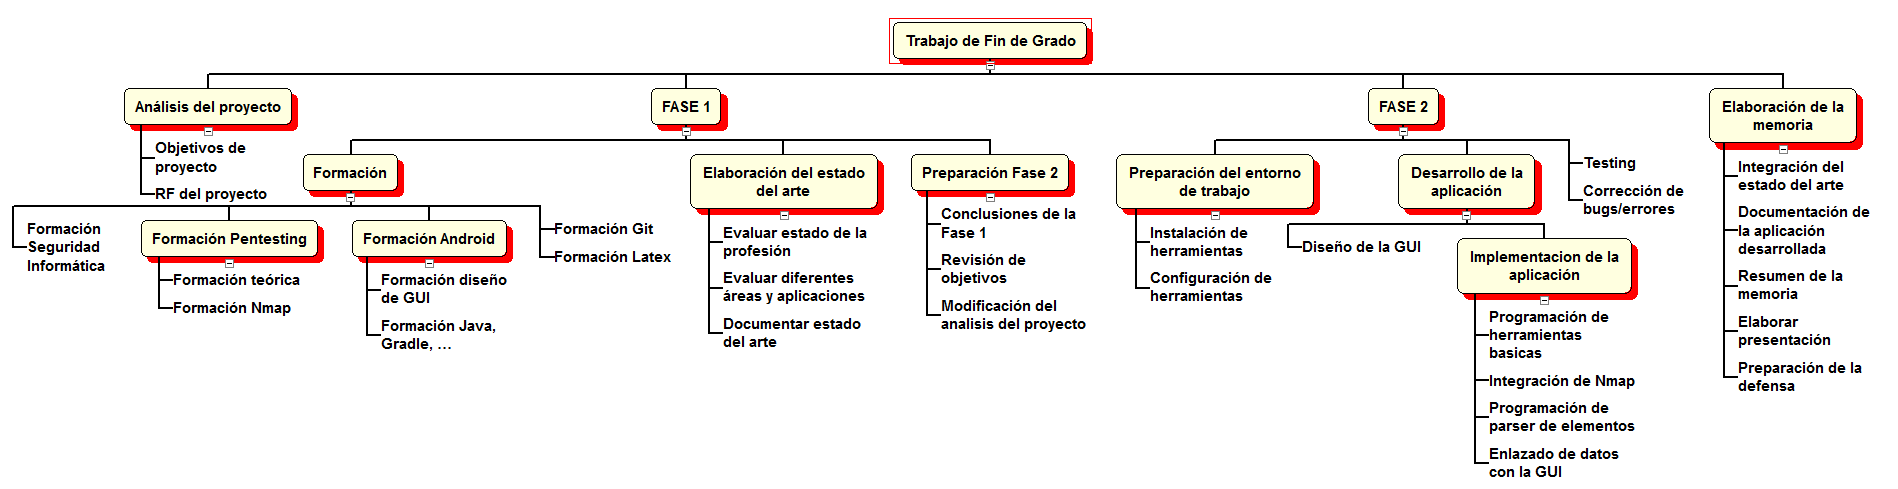
\includegraphics[height=150px]{TFG_EDT}
		\caption{EDT completo}
		\label{fig:edt}
	\end{figure}
	
	\clearpage
	
	\subsubsection{Fase 1}
	El EDT para la Fase 1 quedaría como se muestra en la \autoref{fig:edt1}.
	
	\begin{figure}[H]
		\centering
		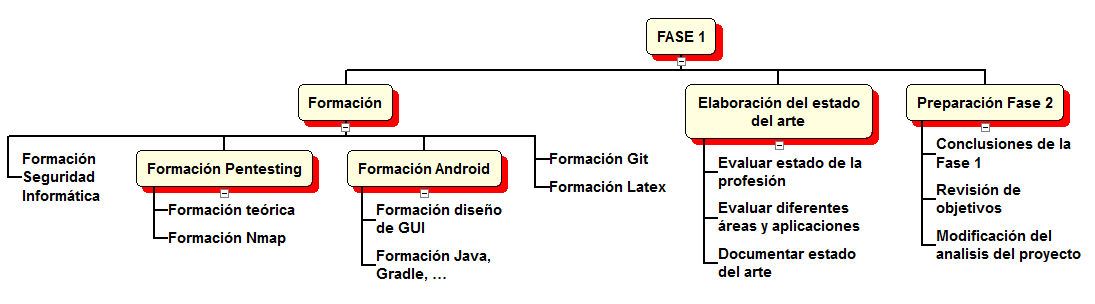
\includegraphics[height=150px]{TFG_EDT_FASE_1}
		\caption{EDT de la Fase 1}
		\label{fig:edt1}
	\end{figure}

\end{landscape}

\subsubsection{Fase 2}
El EDT para la Fase 2 quedaría como se muestra en las \autoref{fig:edt2}.

\begin{figure}[H]
	\centering
	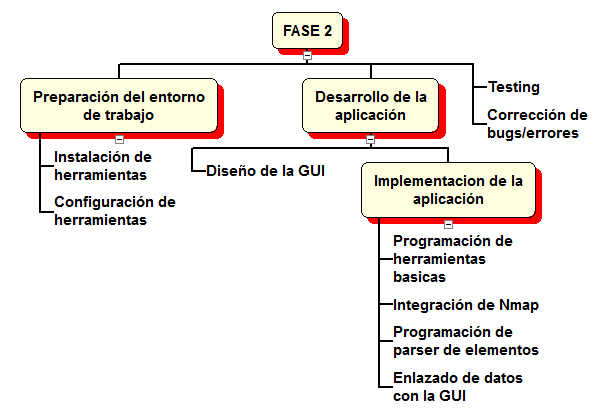
\includegraphics[width=1\textwidth]{TFG_EDT_FASE_2}
	\caption{EDT de la Fase 2}
	\label{fig:edt2}
\end{figure}

\subsection{Agenda del proyecto}
El proyecto se llevará a cabo durante varios meses, comenzando en abril. Se trabajará a media jornada (4 horas) de lunes a viernes, con las siguientes excepciones. Primero, se tendrá en cuenta el calendario de festivos oficiales para aplicar algunas jornadas festivas en cuyos días no se trabajará. Esos días quedan reflejados en la \autoref{table:festivos-oficiales}.

\begin{table}[H]
	\centering
	\begin{tabular}{ |c|c| } 
		\hline
		Fecha & Evento \\
		\hline
		1 de Enero & Año nuevo \\
		6 de Enero & Día de Reyes \\
		19 de Marzo & San José \\
		29 de Marzo & Jueves Santo \\
		30 de Marzo & Viernes Santo \\
		2 de Abril & Lunes de Pascua \\
		28 de Abril & San Prudencio \\
		1 de Mayo & Día del trabajo \\
		25 de Julio & Santiago Apóstol \\
		5 de Agosto & Virgen Blanca \\
		15 de Agosto & Asunción de la Virgen \\
		12 de Octubre & Fiesta Nacional de España \\
		6 de Diciembre & Día de la constitución \\
		8 de Diciembre & Inmaculada Concepción \\
		25 de Diciembre & Navidad \\
		\hline
	\end{tabular}
	\caption{Calendario de días festivos oficial (de Álava)}
	\label{table:festivos-oficiales}
\end{table}

En base a dicho calendario, la fecha estimada de finalización del proyecto es del 16 de enero del 2018.

\subsection{Tareas}
El EDT completo de tareas, al que se añaden la fase inicial de objetivos del proyecto, y toda la fase final de elaboración de la memoria, presentación y la defensa quedaría de la siguiente manera.
\begin{numbered}
	\setcounter{numberedi}{-1} %Para empezar a contar desde 0
	
	\item Análisis del proyecto
	\begin{numbered}
		\item Objetivos del proyecto
		\item RF del proyecto
	\end{numbered}
	
	\item FASE 1
	\begin{numbered}
		
		\item Formación
		\begin{numbered}
			\item Formación seguridad informática
			\item Formación Pentesting
			\begin{numbered}
				\item Formación Teórica
				\item Formación Nmap
			\end{numbered}
			\item Formación Android
			\begin{numbered}
				\item Formación Diseño de GUI
				\item Formación Java, Gradle, ...
			\end{numbered}
			\item Formación Git
			\item Formación \LaTeX
		\end{numbered}
		
		\item Elaboración del estado del arte
		\begin{numbered}
			\item Evaluar estado de la profesión
			\item Evaluar diferentes áreas y aplicaciones
			\item Documentar estado del arte
		\end{numbered}
		
		\item Preparación de la Fase 2
		\begin{numbered}
			\item Conclusiones de la Fase 1
			\item Revisión de objetivos
			\item Modificación del análisis del proyecto
		\end{numbered}
	\end{numbered}
	
	\item FASE 2
	\begin{numbered}
		\item Preparación del entorno de trabajo
		\begin{numbered}
			\item Instalación de herramientas
			\item Configuración de herramientas
		\end{numbered}
		
		\item Desarrollo de la aplicación
		\begin{numbered}
			\item Diseño de la GUI
			\item Implementación de la aplicación
			\begin{numbered}
				\item Programación de herramientas básicas
				\item Integración de Nmap
				\item Programación de parser de elementos
				\item Enlazado de datos con la GUI
			\end{numbered}
			\item Testeo
			\item Corrección de bugs/errores
		\end{numbered}
	\end{numbered}
	
	\item Elaboración de la memoria
	\begin{numbered}
		\item Integración del estado del arte
		\item Documentación de la aplicación desarrollada
		\item Resumen de la memoria
		\item Elaborar presentación
		\item Preparación de la defensa
	\end{numbered}
	
	\item Reuniones periódicas
\end{numbered}

A continuación se explica mediante una breve definición cada tarea, además de especificar su duración en horas.

\taskframe
	{0.1}
	{Objetivos del proyecto}
	{Definir los objetivos que tiene que cumplir el TFG}
	{5}
\taskframe
	{0.2}
	{RF del proyecto}
	{Definir, en base a los objetivos del proyecto, los Requisitos Funcionales (RF) concretos del proyecto}
	{5}
\taskframe
	{1.1.1}
	{Formación seguridad informática}
	{Familiarizarse con el amplio entorno de la seguridad informática y comprender las diferentes áreas, objetivos y el estado de dicho campo}
	{30}
\taskframe
	{1.1.2.1}
	{Formación Teórica}
	{Familiarizarse con los conceptos de Pentesting, las diferentes técnicas usadas y las diferentes fases del proceso de Pentesting}
	{20}
\taskframe
	{1.1.2.2}
	{Formación Nmap}
	{Familiarizarse con el entorno de Nmap, cómo implementarlo, usarlo para obtener información y de qué formas se puede obtener información estructurada y organizada para su posterior uso}
	{10}
\taskframe
	{1.1.3.1}
	{Formación Diseño de GUI}
	{Aprender a usar herramientas de diseño de GUI, diferentes patrones de diseño en sistemas Android, y el uso de IDEs o herramientas para desarrollar dichas GUIs}
	{10}
\taskframe
	{1.1.3.2}
	{Formación Java, Gradle, ...}
	{Aprender sobre el uso de Java para desarrollar aplicaciones Android, diferentes clases, utilidades o conceptos recurrentes en la programación para Android}
	{15}
\taskframe
	{1.1.4}
	{Formación Git}
	{Aprender el uso de dicho sistema de control de versiones para llevar un control riguroso del desarrollo del proyecto y de la aplicación}
	{5}
\taskframe
	{1.1.5}
	{Formación \LaTeX}
	{Aprender diferentes conceptos de \LaTeX para elaborar tanto el estado del arte como el propio informe de la manera más clara y elegante posible}
	{5}
\taskframe
	{1.2.1}
	{Evaluar estado de la profesión}
	{Analizar los diferentes campos de la profesión, las necesidades mas demandadas y los diferentes perfiles de profesionales dentro del campo}
	{5}
\taskframe
	{1.2.2}
	{Evaluar diferentes áreas y aplicaciones}
	{Evaluar las necesidades concretas a nivel técnico, las aplicaciones más usadas y las virtudes y carencias de éstas}
	{10}
\taskframe
	{1.2.3}
	{Documentar estado del arte}
	{Elaborar la documentación en base a toda la información recogida para obtener un elaborado estado del arte}
	{5}
\taskframe
	{1.3.1}
	{Conclusiones de la Fase 1}
	{Elaborar una serie de conclusiones en función a todo el estudio realizado sobre el campo de la seguridad informática}
	{5}
\taskframe
	{1.3.2}
	{Revisión de objetivos}
	{Revisión de los objetivos y los Requisitos Funcionales de la aplicación a desarrollar en función a todo lo investigado}
	{5}
\taskframe
	{1.3.3}
	{Modificación del análisis del proyecto}
	{Modificar la parte de análisis del proyecto realizada anteriormente, antes de comenzar con la Fase 2}
	{5}					
\taskframe
	{2.1.1}
	{Instalación de herramientas}
	{Instalación de todo lo necesario para desarrollar la aplicación}
	{5}
\taskframe
	{2.1.2}
	{Configuración de herramientas}
	{Configuración de todas las herramientas para que el desarrollo de la aplicación sea lo mas cómodo posible}
	{5}
\taskframe
	{2.2.1}
	{Diseño de la GUI}
	{Diseñar una interfaz gráfica clara y sencilla de usar para interactuar con las funciones a implementar}
	{15}
\taskframe
	{2.2.2.1}
	{Programación de herramientas básicas}
	{Programar herramientas básicas para el escaneo de redes}
	{10}
\taskframe
	{2.2.2.2}
	{Integración de Nmap}
	{Integrar el núcleo de Nmap en la aplicación para poder hacer uso de toda su funcionalidad}
	{10}
\taskframe
	{2.2.2.3}
	{Programación de parser de elementos}
	{Elaborar un puente entre Nmap y la aplicación para obtener los datos de Nmap y poder usarlos en la aplicación de la manera más organizada posible}
	{20}
\taskframe
	{2.2.2.4}
	{Enlazado de datos con la GUI}
	{Enlazar los datos con las diferentes vistas a través de diversos controladores, para poder visualizar e interactuar con ellos}
	{15}
\taskframe
	{2.2.3}
	{Testing}
	{Una vez desarrollada la aplicación, realizar un amplio testeo para comprobar que funciona correctamente}
	{10}
\taskframe
	{2.2.4}
	{Corrección de bugs/errores}
	{En base a los errores detectados en el testeo, implementar las correcciones a dichos fallos}
	{15}
\taskframe
	{3.1}
	{Integración del estado del arte}
	{Integrar el estado del arte desarrollado dentro de la memoria}
	{5}
\taskframe
	{3.2}
	{Documentación de la aplicación desarrollada}
	{Elaborar en base a todo el proceso de desarrollo una documentación clara sobre la aplicación e integrarla en la memoria}
	{15}
\taskframe
	{3.3}
	{Resumen de la memoria}
	{Terminar la elaboración de la memoria, añadiendo las diferentes secciones necesarias y el formato correspondiente}
	{5}
\taskframe
	{3.4}
	{Elaborar presentación}
	{Elaborar la presentación en diapositivas que se usará en la defensa ante el tribunal}
	{5}
\taskframe
	{3.5}
	{Preparación de la defensa}
	{Preparar la defensa ante el tribunal en función a la documentación elaborada}
	{10}
\taskframe
	{4}
	{Reuniones periódicas}
	{Reuniones periódicas con el director del TFG para llevar un control del desarrollo del proyecto}
	{15}

\subsection{Entregables}

\subsubsection{Fase 1}
El entregable de la Fase 1 consistirá en un estado del arte redactado sobre el campo de la seguridad informática que analice cuales son las amenazas existentes, los diferentes campos de enfoque y las técnicas actuales para securizar sistemas, haciendo especial hincapié en el pentesting

\subsubsection{Fase 2}
El entregable de la Fase 2 consistirá en una aplicación elaborada, que sirva como herramienta para el escaneo de redes informáticas. La aplicación, desarrollada para Android, estará correctamente empaquetada, con los posible fallos corregidos y además dispondrá de una GUI sencilla de usar.

\subsection{Cronograma}
El cronograma completo, con las dos fases, se muestra en las Figuras \ref{fig:gantt0}, \ref{fig:gantt1}, \ref{fig:gantt2} y \ref{fig:gantt3}.

\begin{figure}[H]
	\centering
	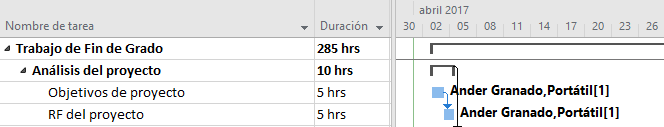
\includegraphics[width=1\textwidth]{TFG_GANTT_FASE_0}
	\caption{Cronograma de la fase inicial}
	\label{fig:gantt0}
\end{figure}

\begin{landscape}

\begin{figure}[H]
	\centering
	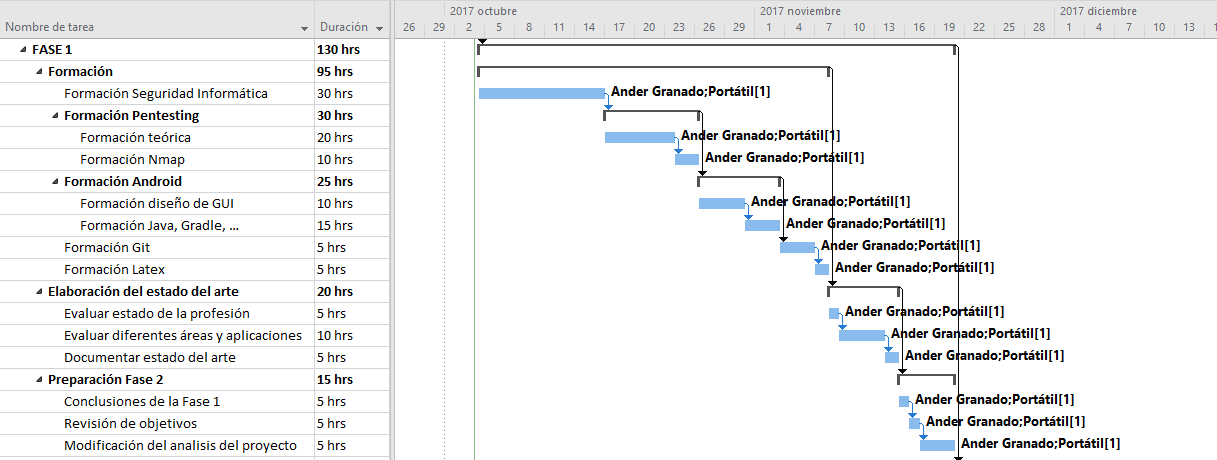
\includegraphics[height=210px]{TFG_GANTT_FASE_1}
	\caption{Cronograma de la Fase 1}
	\label{fig:gantt1}
\end{figure}

\begin{figure}[H]
	\centering
	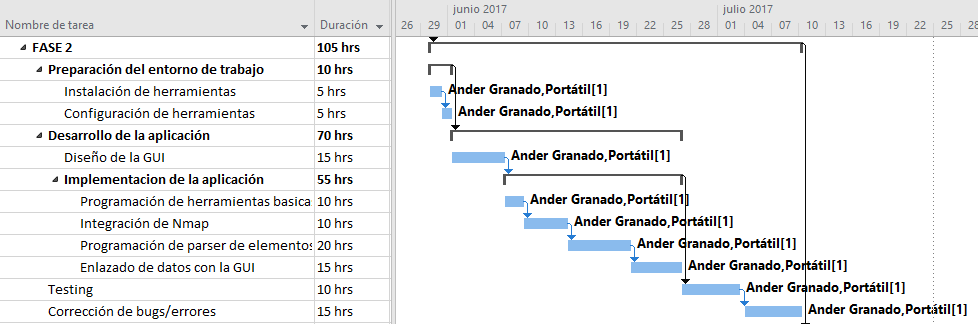
\includegraphics[height=160px]{TFG_GANTT_FASE_2}
	\caption{Cronograma de la Fase 2}
	\label{fig:gantt2}
\end{figure}

\end{landscape}

\begin{figure}[H]
	\centering
	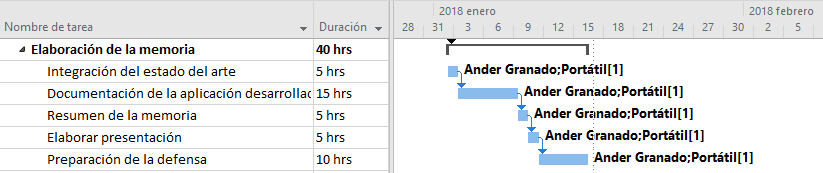
\includegraphics[width=1\textwidth]{TFG_GANTT_FASE_3}
	\caption{Cronograma de la elaboración de la memoria}
	\label{fig:gantt3}
\end{figure}



%------------------------------------------------------------------------------


\section{Gestión de costos}
A la hora de elaborar un análisis de costos, con el objetivo de obtener un presupuesto, primero es necesario identificar todos los recursos que influyen en ese presupuesto. Por una parte, tendremos los recursos de trabajo, es decir empelados, y por otra parte los recursos materiales, tanto de software como de hardware. En la \autoref{fig:recursos} se muestran tanto los recursos de trabajo como los recursos materiales de hardware.

\begin{figure}[H]
	\centering
	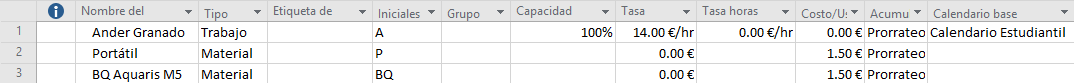
\includegraphics[width=1\textwidth]{TFG_RECURSOS}
	\caption{Recursos de trabajo y materiales}
	\label{fig:recursos}
\end{figure}

Por otra parte, en la \autoref{table:software} se muestra los recursos materiales de software utilizados.

\begin{table}[H]
	\centering
	\begin{tabular}{ |l|r| } 
		\hline
		\multicolumn{1}{|c|}{Concepto} & 
			\multicolumn{1}{|c|}{Coste} \\
		\hline
		Windows 10 		& 135,00 \euro \cite{precio-win10}		\\
		Project 2016 	& 1.369,00 \euro \cite{precio-project}	\\
		WBS Chart Pro 	& 187,50 \euro \cite{precio-wbs}		\\
		Ubuntu 16.04 	& 0,00 \euro							\\
		TeX Studio 		& 0,00 \euro							\\
		Android Studio 	& 0,00 \euro							\\
		Nmap 			& 0,00 \euro							\\
		Git 			& 0,00 \euro							\\
		GitHub 			& 0,00 \euro							\\
		\hline
	\end{tabular}
	\caption{Recursos materiales (software)}
	\label{table:software}
\end{table}


\subsection{Presupuesto}
El análisis de costes del proyecto se refleja en toda la información que aparecen entre la \autoref{table:recursos-trabajo} y la \autoref{table:total-presupuesto}. Para ello se tienen en cuanta varios puntos. El primero, se tiene en cuenta un salario base de 14 \euro/h, correspondiente un salario estándar de un analista programador.
Para los recursos materiales, se tiene en cuenta un costo por uso de 1,50 \euro. Estos costos por uso vienen dados por el gasto que generan debido al consumo energético, internet y otro tipo de gastos derivados de su utilización. Por otra parte se realiza una separación para los recursos de software, entre los que se incluye el propio Microsoft Project, software usado para la realización de todo el análisis de viabilidad y la gestión del proyecto.
Para el cálculo de las amortizaciones se considera un tiempo de amortización de 3 años, el cual traducido en horas vendría a ser 4800 horas ($3\ a\tilde{n}os\ *\ 200\ d\acute{i}as\ laborables\ *\ 8\ horas\ =\ 4800\ horas$).

\begin{table}[H]
	\centering
	\begin{tabular}{ |l|r| } 
		\hline
		\multicolumn{1}{|c|}{Concepto} & 
			\multicolumn{1}{|c|}{Coste} \\
		\hline
		Ander Granado & 14,00 \euro/h \\
		\hline
	\end{tabular}
	\caption{Recursos de trabajo}
	\label{table:recursos-trabajo}
\end{table}

\begin{table}[H]
	\centering
	\begin{tabular}{ |l|r| } 
		\hline
		\multicolumn{1}{|c|}{Concepto} & 
			\multicolumn{1}{|c|}{Coste} \\
		\hline
		Ordenador portátil 	& 700,00 \euro \\
		BQ Aquaris M5 		& 250,00 \euro \\
		\hline
	\end{tabular}
	\caption{Recursos materiales (hardware)}
	\label{table:recursos-materiales}
\end{table}

\begin{table}[H]
	\centering
	\begin{tabular}{ |l|r|r| } 
		\hline
		\multicolumn{1}{|c|}{Concepto} & 
			\multicolumn{1}{|c|}{Coste} & 
				\multicolumn{1}{|c|}{Número de licencias} \\
		\hline
		Windows 10 		& 135,00 \euro \cite{precio-win10} 		& 1 \\
		Project 2016 	& 1369,00 \euro \cite{precio-project} 	& 1 \\
		WBS Chart Pro 	& 187,50 \euro \cite{precio-wbs} 		& 1 \\
		Ubuntu 16.04 	& 0,00 \euro 							& 1 \\
		TeX Studio 		& 0,00 \euro							& 1 \\
		Android Studio 	& 0,00 \euro 							& 1 \\
		NMap 			& 0,00 \euro 							& 1 \\
		Git 			& 0,00 \euro 							& 1 \\
		GitHub 			& 0,00 \euro 							& 1 \\
		\hline
	\end{tabular}
	\caption{Recursos materiales (software)}
	\label{table:recursos-software}
\end{table}

\begin{table}[H]
	\centering
	\begin{tabular}{ |l|r|r|r|r|r| } 
		\hline
		\multicolumn{1}{|c|}{Concepto} & 
			\multicolumn{1}{|c|}{Trabajo (h)} & 
				\multicolumn{1}{|c|}{Trabajo horas extra} & 
					\multicolumn{1}{|c|}{Coste} & 
						\multicolumn{1}{|c|}{Coste horas extra} & 
							\multicolumn{1}{|c|}{Importe} \\
		\hline
		Ander Granado & 285 & 0 & 14,00 \euro/h & 0 & 4.044,00 \euro \\
		\hline
	\end{tabular}
	\caption{Costo de recursos de trabajo}
	\label{table:costo-recursos-trabajo}
\end{table}

\begin{table}[H]
	\centering
	\begin{tabular}{ |l|r|r|r| } 
		\hline
		\multicolumn{1}{|c|}{Concepto} & 
			\multicolumn{1}{|c|}{Unidades} & 
				\multicolumn{1}{|c|}{Coste} & 
					\multicolumn{1}{|c|}{Importe} \\
		\hline
		Ordenador portátil 	& 1 & 1,50 \euro/uso & 29 x 1,50 \euro \space= 43,50 \euro	\\
		BQ Aquaris M5 		& 1 & 1,50 \euro/uso & 7 x 1,50 \euro \space= 10,50 \euro	\\
		\hline
		\multicolumn{3}{|l}{TOTAL} & \multicolumn{1}{r|}{54,00 \euro} \\ 
		\hline
	\end{tabular}
	\caption{Costo de recursos materiales}
	\label{table:costo-recursos-materiales}
\end{table}

\begin{table}[H]
	\centering
	\begin{tabular}{ |l|r|r|r|r|r| } 
		\hline
		\multicolumn{1}{|c|}{Concepto} & 
			\multicolumn{1}{|c|}{Coste unitario} & 
				\multicolumn{1}{|c|}{T. de Amort.\tablefootnote{Tiempo de amortización}} & 
					\multicolumn{1}{|c|}{C.U.A.\tablefootnote{Coste unitario de amortización} (\euro)} & 
						\multicolumn{1}{|c|}{T. de uso} & 
							\multicolumn{1}{|c|}{Importe} \\
		\hline
		Ordenador portátil 		& 700,00 \euro 	& 4800 horas & 0,145833 \euro & 285 h	& 41,57 \euro	\\
		BQ Aquaris M5 			& 250,00 \euro 	& 4800 horas & 0,052083 \euro & 25 h	& 1,30 \euro	\\
		Windows 10 				& 135,00 \euro 	& 4800 horas & 0,028125 \euro & 180 h	& 5,06 \euro	\\
		M. Project 2016 	& 1.369,00 \euro & 4800 horas & 0,285208 \euro & 25 h	& 7,13 \euro 	\\
		WBS Chart Pro 			& 187,50 \euro 	& 4800 horas & 0,039062 \euro & 5 h		& 0,19 \euro	\\
		Ubuntu 16.04 			& 0,00 \euro 	& 4800 horas & 0,000000 \euro & 105 h	& 0,00 \euro	\\
		TeX Studio 				& 0,00 \euro 	& 4800 horas & 0,000000 \euro & 40 h	& 0,00 \euro	\\
		Android Studio 			& 0,00 \euro 	& 4800 horas & 0,000000 \euro & 105 h	& 0,00 \euro	\\
		NMap 					& 0,00 \euro 	& 4800 horas & 0,000000 \euro & 30 h	& 0,00 \euro	\\
		Git 					& 0,00 \euro 	& 4800 horas & 0,000000 \euro & 145 h	& 0,00 \euro	\\
		GitHub 					& 0,00 \euro 	& 4800 horas & 0,000000 \euro & 145 h	& 0,00 \euro	\\
		\hline
		\multicolumn{5}{|l}{TOTAL} & \multicolumn{1}{r|}{55,25 \euro} \\ 
		\hline
	\end{tabular}
	\caption{Amortizaciones de hardware y software}
	\label{table:amortizaciones}
\end{table}

\begin{table}[H]
	\centering
	\begin{tabular}{ |l|r| } 
		\hline
		\multicolumn{1}{|c|}{Concepto} & 
			\multicolumn{1}{|c|}{Importe} \\
		\hline
		Recursos de Trabajo (R.T.)	& 4.044,00 \euro	\\
		Recursos Materiales (R.M.)	& 54,00 \euro		\\
		Costo fijo					& 0,00 \euro		\\
		Amortizaciones				& 55,25 \euro		\\
		\hline
		SUMA						& 4.153,25 \euro	\\
		\hline
		Gastos generales (10\%)		& 415,32 \euro		\\
		Beneficio (15\%)			& 622,99 \euro		\\
		\hline
		SUBTOTAL					& 5.191,56 \euro	\\
		IVA (21\%)					& 1.090.23 \euro	\\
		\hline
		TOTAL						& 6281.79 \euro		\\
		\hline
	\end{tabular}
	\caption{Total presupuesto}
	\label{table:total-presupuesto}
\end{table}

Con esto se concluye que, tal como figura en la \autoref{table:total-presupuesto}, el coste del proyecto asciende a la cantidad de \textit{seis mil doscientos ochenta y cinco con setenta y nueve euros} (6281.79 \euro).

%------------------------------------------------------------------------------

\section{Gestión de riesgos}

En este apartado se identifican y analizan las diferentes amenazas que puedan llegar a impedir el correcto desarrollo del proyecto, haciendo que éste se retrase. Para ello primero se identifican los diferentes riesgos que pueden existir y se indica su peligrosidad. La peligrosidad es un valor cualitativo que indica en que medida puede afectar ese riesgo al proyecto.

Se han identificado los siguientes riesgos, los cuales se muestran en la \autoref{table:riesgos}.

\begin{table}[H]
	\centering
	\begin{tabular}{ |l|c| } 
		\hline
		\multicolumn{1}{|c|}{Riesgo} & 
		\multicolumn{1}{|c|}{Peligrosidad} \\
		\hline
			Pérdida de información										& Alta	\\
			Enfermedades												& Alta	\\
			Dificultades en la implementación de la aplicación			& Alta	\\
			Dedicación no exclusiva al trabajo							& Media	\\
			Averías o problemas técnicos con los recursos materiales	& Media	\\
			Cambios o ampliación de requisitos							& Media	\\
			Planificación muy optimista									& Media	\\
		\hline
	\end{tabular}
	\caption{Enumeración de riesgos del proyecto}
	\label{table:riesgos}
\end{table}


\subsection{Explicación y plan de contingencia}
Tras haber identificado los riesgos inherentes al proyecto en la \autoref{table:riesgos}, se hace mayor hincapié en los detalles de dicho riesgos, elaborando una descripción más detallada y analizando su probabilidad. La probabilidad de cada riesgo se muestra de manera cualitativa, ya que aportar un valor numérico concreto en este tipo de casos resulta bastante complicado. También, junto a lo mencionado, se añade para cada riesgo un plan de contingencia. El plan de contingencia consiste básicamente en aportar medidas para afrontar dicho riesgo, tanto preventivas (para antes de que ocurra) como correctoras (para en caso de ocurrir).

\riskframe
	{Pérdida de información}
	{Podría darse el caso de que parte de la información, como la memoria del proyecto, el estado del arte o el código de la aplicación se perdieran}
	{Baja}
	{Alta}
	{Uso de herramientas de control de versiones como Git junto a uso de herramientas cloud como GitHub o Dropbox}
	{Recuperación de la información mediante herramientas de análisis de unidades}

\riskframe
	{Enfermedades}
	{Podría suceder que el único recurso de trabajo contrajera una enfermedad o tuviera un accidente}
	{Baja}
	{Alta}
	{Ninguna}
	{Usar horas fuera del calendario para corregir el retraso en el proyecto}


\riskframe
	{Dificultades en la implementación de la aplicación}
	{Podría suceder que, durante la implementación de la aplicación, se dieran dificultades a nivel de programación a la hora de cumplir con los Requisitos Funcionales}
	{Media}
	{Alta}
	{Una formación sólida en las herramientas y tecnologías que se van a usar para el desarrollo de la aplicación}
	{Replantear las tareas posteriores y dedicar un esfuerzo extra para el aprendizaje y refuerzo de las herramientas usadas}

\riskframe
	{Dedicación no exclusiva al trabajo}
	{Podría suceder que, debido a exámenes u otros asuntos personales, el desarrollador no pudiera aportar toda la dedicación que requiere el proyecto}
	{Media}
	{Media}
	{No previsible}
	{Cambiar calendario de trabajo aumentando las horas para subsanar los retrasos producidos por dicho riesgo}

\riskframe
	{Averías o problemas técnicos con los recursos materiales}
	{Podría darse el caso de que alguno de los recursos materiales de hardware, como el ordenador o el teléfono móvil, sufran algún tipo de avería}
	{Baja}
	{Media}
	{No previsible}
	{Uso de otros dispositivos para continuar con el desarrollo del proyecto, adquiridos mediante compra o préstamo}

\riskframe
	{Cambios o ampliación de requisitos}
	{Podría darse el caso en el que, tras la conclusión de la Fase 1, se cambiarán Requisitos Funcionales de la aplicación a desarrollar o se añadirán nuevos Requisitos Funcionales}
	{Media - Alta}
	{Media}
	{Revisión constante de los Requisitos Funcionales durante todas las fases del proyecto para minimizar el impacto que pueda causar los cambios en ellos}
	{Adaptar el calendario las tareas posteriores y el calendario de trabajo actual}

\riskframe
	{Planificación muy optimista}
	{Puede darse el caso de que la planificación elaborada para el proyecto sea demasiado optimista y no haya tenido en cuenta ciertos aspectos más concretos del desarrollo del proyecto}
	{Media}
	{Media}
	{No previsible}
	{Adaptar, y en caso de que fuera necesario retrasar, la fecha final del proyecto para dar cabida en la planificación toda  esa duración extra no prevista}

\part{Fase 1: Estado del Arte de la Seguridad Informática}
\chapter{Introducción}

La siguiente parte de esta memoria contiene el trabajo realizado durante la Fase 1 del proyecto. En él se elabora un completo estado del arte sobre el mundo de la seguridad informática. Dicho estado del arte se encuentra dividido en cuatro capítulos.

En el primero, simplemente se pasa a mencionar una serie de conceptos básicos sobre seguridad informática, definiciones que resulta fundamental comprender sobre este área de la informática.

En el segundo capítulo, llamado \textit{Aplicaciones de la Seguridad Informática}, se enumeran una serie de amenazas hacia la seguridad, pasando de un enfoque más clásico a profundizar en las áreas con más auge dentro del campo, mostrando sus particularidades, con el objetivo de hacerse una visión global de las diferentes necesidades y de cómo la seguridad informática se aplica en cada campo.

En el tercer capítulo, denominado \textit{Pentesting}, se profundiza en la técnica que su propio nombre indica. Dicha técnica es una de las herramientas fundamentales de la seguridad informática, y permite obtener una mejor visión de como securizar sistemas.

Aun así, el objetivo de este estado del arte no es simplemente obtener una visión global del campo de la seguridad informática, sino también ser capaces de extraer una serie de conclusiones con el objetivo final de ofrecer una solución que consiga hacer que el propio usuario, inexperto, pero el principal \textit{target} de cualquiera de las tecnologías de la información, tenga un papel proactivo en la seguridad de sus sistemas y su información.

De esta manera, de una visión vaga y difuminada de un campo con cada vez mayor importancia, se obtendrá una imagen nítida de todo el área, que además permita enfocar la solución a desarrollar.
\chapter{Conceptos Generales}

\epigraph{\textit{''El único sistema verdaderamente seguro es aquel que se encuentra apagado, enterrado en un bloque de hormigón en una habitación sellada con plomo y vigilada por guardias armados. Incluso entonces tendría mis dudas''}}{--- Gene Spafford}

Tal y como Gene Spafford asegura con sus palabras \cite{gene-spafford}, la seguridad informática no es una ciencia infalible, y el sistema verdaderamente seguro es una quimera, algo que no existe y es inalcanzable. Con esto de base, la seguridad informática tiene diversos objetivos que surgen de la necesidad de proteger la información y los sistemas informáticos cada vez más en auge. Objetivos como minimizar y gestionar los riesgos y detectar los posibles problemas y amenazas de seguridad, garantizar la utilización adecuada del sistema y la información, limitar las pérdidas y conseguir a la adecuada recuperación del sistema en caso de un incidente de seguridad, cumplir con el marco legal los requisitos impuestos por los clientes en sus contratos, etc.

Existen numerosas definiciones para el término seguridad informática. En esencia, la seguridad informática es el área de la informática que se enfoca tanto en la protección de sistemas como en la protección de la propia información.

Resulta necesario distinguir entre dos conceptos. Por una parte tenemos el concepto es seguridad informática, y por otra parte el concepto de seguridad de la información. Aunque al principio ambos conceptos pueden parecer sinónimos, se tratan de áreas diferentes.

%------------------------------------------------------------------------------

\section{Seguridad Informática}

Existen un gran número de definiciones para la seguridad informática. Según INTECO \cite{inteco-defs}, Instituto Nacional de Tecnologías de la Comunicación, ahora INCIBE) la seguridad informática consiste en la protección de las infraestructuras TIC que soportan un negocio o empresa. En la nomra ISO 7498 \cite{iso-7498}, en la que se recoge el modelo OSI (modelo de referencia creado en 1980 para arquitecturas de red, en contraposición a la heterogeneidad del modelo TCP/IP), se define la seguridad informática como una serie de mecanismos que minimizan la vulnerabilidad de bienes y recursos en una organización.

Aunque existen gran cantidad de definiciones para el concepto de seguridad informática, por lo general engloban el carácter de protección de cualquier tipo de recurso tecnológico informático, muchas veces supeditado a s uso en una organización. Aunque no tiene porqué ser así. También existen discrepancias entre sí considerar la propia información como uno de esos recursos a proteger. 

%------------------------------------------------------------------------------

\section{Seguridad de la Información}

A la par que el concepto de seguridad informática, surge el concepto de seguridad de la información. Según INTECO \cite{inteco-defs}, la seguridad de la información consiste en la protección de los activos de información fundamentales para el éxito de cualquier organización.

En una definición más antigua, elaborada en la norma ISO/IEC 17799 \cite{iso-17799} se define la seguridad de la información como la preservación de la CID, acrónimo de “Confidencialidad, Integridad y Disponibilidad” (en inglés CIA, “Confidentiality, Integrity, Availability”). El concepto de CID es uno de los pilares de la seguridad de la información, en el que se ahondará más adelante.

Mientras que la seguridad informática se encarga de proteger las infraestructuras, es decir, se basa en un plano más técnico, la seguridad de la información no tiene porqué hacer referencia a ningún tipo de tecnología informática o de comunicación. Los activos de información puede ser digitales, como correos electrónicos, páginas web, imágenes, bases de datos, …  pero no  tiene por qué ser necesariamente así. También se puede clasificar como activo de  de información documentos en papel contratos, faxes, etcétera.

Al igual que ocurre con la seguridad informática, es habitual tratar el término de la seguridad de la información a nivel empresarial, cuando no está exclusivamente ligado a ese campo.

%------------------------------------------------------------------------------

\section{Servicios de la Seguridad de la Información}
La seguridad de la información proporciona una serie de servicios que tienen como objetivo proteger todo tipo de activos de información, ya sea de una organización o de un usuario particular. La suma y complementación de estos servicios es lo que permite esa completa protección de la información.

\subsection[CID]{Confidencialidad, Integridad y Disponibilidad}

Dentro de estos servicios, existe el acrónimo CID, Confidencialidad, Integridad, Disponibilidad. CID engloba los 3 servicios de la seguridad de la información más importantes existentes \cite{iso-27000}.

\begin{figure}[H]
	\centering
	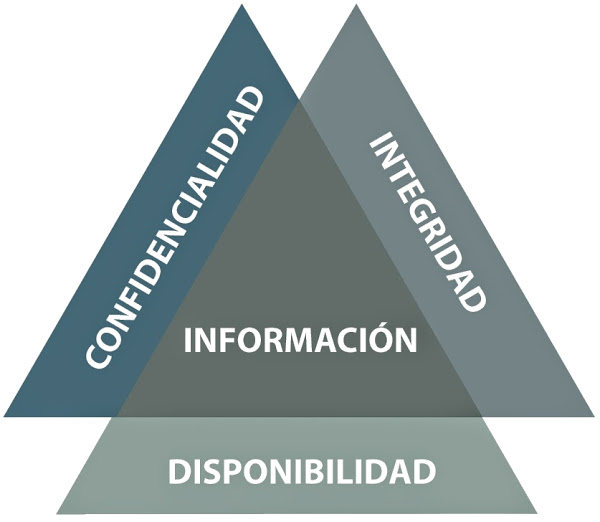
\includegraphics[width=200px]{cid}
	\caption{Confidencialidad, Integridad y Disponibilidad}
	\label{fig:cid}
\end{figure}

\begin{itemize}
	\item \emph{Confidencialidad}: garantiza que la información no se pone a disposición ni se revela  a individuos, entidades o procesos no autorizados.
	\item \emph{Integridad}: garantiza que la información no se modifica malintencionadamente, por parte de individuos o procesos, durante su procesado o su transmisión, y en caso de modificarse, permite detectar dichas modificaciones.
	\item \emph{Disponibilidad}: garantiza el acceso y utilización de la información y los sistemas de tratamiento de la misma por parte de los individuos, entidades o procesos autorizados cuando lo requieran. Además garantiza la recuperación de la información y de los sistemas de información en caso de posibles incidentes.
\end{itemize}

\subsection{Otros servicios}

Además de CID, existen otros servicios que complementan el concepto de seguridad informática. Aunque CID consiste en tres servicios que son de obligado cumplimiento para garantizar la seguridad de la información, no resultan suficientes, ya que no cubren todo tipo de casos en los que se puede comprometer la información. Entre el diverso número  que existen, se enumera y define una serie de ellos, considerados de los más relevantes \cite{apuntes-isma}.

\begin{itemize}
	\item \emph{Confidencialidad:} garantiza que la información no se pone a disposición ni se revela  a individuos, entidades o procesos no autorizados.
	\item \emph{Integridad:} garantiza que la información no se modifica malintencionadamente, por parte de individuos o procesos, durante su procesado o su transmisión, y en caso de modificarse, permite detectar dichas modificaciones.
	\item \emph{Disponibilidad:} garantiza el acceso y utilización de la información y los sistemas de tratamiento de la misma por parte de los individuos, entidades o procesos autorizados cuando lo requieran. Además garantiza la recuperación de la información y de los sistemas de información en caso de posibles incidentes.
\end{itemize}

\begin{itemize}
	\item \emph{Autenticación:} garantiza que la identidad del creador de un mensaje es legítima. Permite asegurar la autoría de la información creada o modificada.
	\item \emph{No repudio:} permite, mediante diferentes mecanismos, demostrar la autoría de un mensaje e impide que el usuario niegue esa circunstancia.
	\item \emph{Autorización:} permite controlar el acceso a cierto sistema o información por parte de un usuario, permitiendo dicho acceso sólo a ciertos usuarios previamente designados, una vez superado el servicio de autenticación. 
	\item \emph{Auditabilidad:} permite registrar y monitorizar la utilización de los distintos recursos del sistema por parte de los usuarios para garantizar el correcto uso del sistema y de su información
	\item \emph{Anonimato:} permite garantizar el anonimato de los usuarios que acceden a los recursos y consumen determinados tipos de servicios, preservando así su privacidad. Puede entrar en conflicto con otros ya mencionados, como la autenticación o la auditoría del acceso a los recursos.
	\item \emph{Protección a la réplica:} impide que se haga uso de ataques de repetición que engañen al sistema provocando operaciones y modificaciones de la información no deseadas.
\end{itemize}

\chapter[Aplicaciones]{Aplicaciones de la Seguridad Informática}

\epigraph{\textit{''Las organizaciones gastan millones de dólares en firewalls y dispositivos de seguridad, pero tiran el dinero porque ninguna de estas medidas cubre el eslabón más débil de la cadena de seguridad: la gente que usa y administra los ordenadores''}}{--- Kevin Mitnick}

Con el objetivo de garantizar todos esos servicios mencionados en el capítulo anterior, se han desarrollado una gran cantidad de áreas dentro de la propia seguridad informática, que permiten cumplir con estos objetivos.

Las áreas de investigación y los campos de trabajo dentro de la seguridad informática avanzan a un ritmo acelerado debido al propio avance de la informática. El desarrollo de áreas como los smartphones o el Internet of Things (IoT) hace necesario nuevas técnicas que permitan garantizar la seguridad de la información a todos los niveles. Áreas como el ransomware, los wearables, los automóviles o el ciberespionaje son algunas en las que más hincapié se está haciendo en los últimos años \cite{mcafee-predictions}.

Teniendo eso en cuenta, durante este capitulo se describirán diferentes tipos de amenazas, tras lo cual se elaborará un análisis en mayor profundidad de las principales áreas que preocupan en el momento actual a la seguridad informática, que son los smartphones, el Internet of Things y el Cloud Computing.

%------------------------------------------------------------------------------

\section{Malware}

La seguridad informática siempre se ha relacionado con el concepto de virus informático. Si bien uno de los objetivos de la seguridad informática es evitar que este tipo de software consiga acceder a información o dañar sistemas, los virus informáticos no son la única manera que existe para comprometer la seguridad de la información. Sin embargo, el campo de la seguridad informática se desarrolla después de que surgieran estas primeras piezas de malware. Es precisamente debido al surgimiento de estas que se comprende la necesidad de desarrollar toda una serie de técnicas para garantizar la seguridad de la información almacenada y procesada en estos sistemas.

El concepto de malware es relativamente novedoso. El origen de programas capaces de replicarse y distribuirse se remonta hacia 1949, cuando el mismísimo Von Neumann expuso \emph{La Teoría y Organización de Autómatas Complejos} \cite{von-neumann}, en la cual habla sobre pequeños autómatas capaces de replicarse por sí solos. Dos décadas después, concretamente en 1971, nace el denominado como primer virus informático de la historia, llamado \emph{Creeper} \cite{creeper} (enredadera en inglés).  Dicho virus no se puede considerar malware como tal ya que no causaba daño a los sistemas en los que se replicaba, simplemente mostraba un inofensivo mensaje a los usuarios (\textsl{''Soy una enredadera... ¡atrápame si puedes!''}). Para contrarrestar dicho virus surgió \emph{Reaper} (segadora en inglés), el cual a día de hoy es denominado como el primer antivirus de la historia. Sin embargo, no es hasta 1984 cuando Frederick B. Cohen acuña por primera vez el término virus informático en uno de sus estudios, definiéndolo como \emph{''Programa que puede infectar a otros programas incluyendo una copia posiblemente evolucionada de sí mismo''} \cite{panda-virus-history}, realizando una analogía con el mundo de la biología.

No es hasta la década de los 80, en la cual los ordenadores personales empezaron a emerger en los hogares, cuando se comienzan a desarrollar virus informáticos a los que sí que podemos considerar maliciosos. Ejemplos famosos son el virus \emph{Viernes 13} en 1987 o el gusano \emph{Happy} en 1999 \cite{panda-virus-history}. Desde la década de los 80 y hasta la actualidad se han ido desarrollando este tipo de virus informáticos, los cuales podemos clasificar como malware.

Cabe mencionar que el malware en sí no tiene porque tener la capacidad para replicarse; se puede considerar malware cualquier pieza de software que busque un uso malintencionado o malicioso del sistema.

Dentro de la categoría de malware se han ido desarrollando diferentes piezas de software que tienen sus particularidades. Dependiendo de su funcionamiento o de los usos para los que esté diseñado el malware se puede clasificar en diferentes categorías, algunas de las cuales tienen mayor auge que otras a día de hoy. En la figura \ref{fig:malware-symantec} se puede observar una serie de datos del crecimiento y descenso de diferentes tipos de malware durante los últimos años.

\begin{figure}[H]
	\centering
	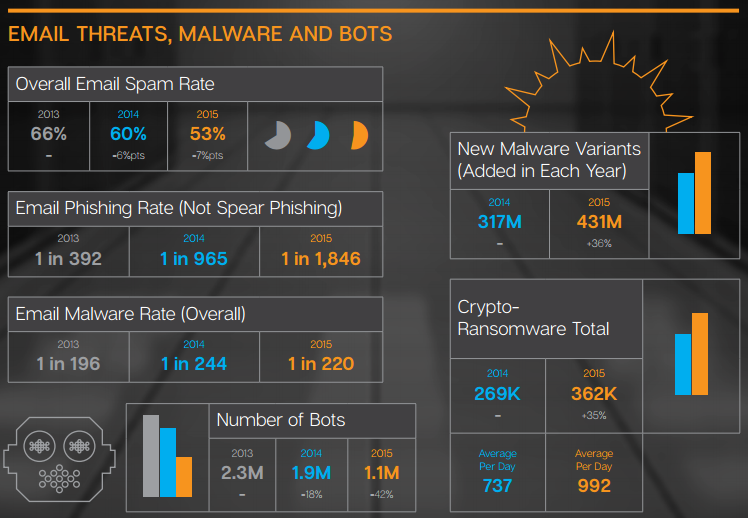
\includegraphics[width=1\textwidth]{malware-symantec}
	\caption{Infografía sobre el malware en 2016 \cite{malware-symantec}}
	\label{fig:malware-symantec}
\end{figure}

\subsection{Gusanos}

Una de las primeras categorías de malware que surge es la de los gusanos. Los gusanos (también conocidos como \textit{worms} por su término en inglés) son programas autorreplicantes que, en vez de infectar archivos concretos, se instalan directamente en los sistemas y buscan, mediante diferentes vulnerabilidades en los sistemas o técnicas como la ingeniería social, replicarse en la medida en la que les sea posible.

Fueron uno de los primeros tipos de malware y a su vez una de las causas principales del desarrollo de la seguridad informática más defensiva. Un ejemplo es el famoso gusano \emph{ILOVEYOU} \cite{top-10-viruses}, el cual infectó en el año 2000 a decenas de millones de ordenadores con Windows. Otros también famosos son \emph{Code red}, \emph{Sasser} o \emph{Conficker}. Son uno de los tipos de malware que mayor daño económico han causado, causando daños estimados en miles de millones de euros solamente teniendo en cuenta los casos mencionados.

Hoy en día, aunque siguen considerándose una amenaza, han quedado relegados a un segundo plano, por una parte, por la capacidad de los sistemas de firewall o sistemas antivirus de detectarlos y neutralizarlos y, por otra parte, por el surgimiento de otros tipos de malware, como los que se mencionan en los siguientes puntos.

\subsection{Troyanos}

Otro tipo de malware famoso son los troyanos. El nombre de troyano proviene del caballo de Troya, una gran estructura de madera que usó el pueblo griego en la guerra de Troya para introducir a sus soldados en la ciudad, que estaba completamente fortificada. De la misma manera, el malware denominado troyano se camufla, es decir, se oculta como un programa legítimo imitando el comportamiento de dicho programa, cuando en realidad son una forma para dar acceso a un atacante a los recursos de dicho sistema. Uno de los troyanos mas famosos fue \emph{Zeus} \cite{top-10-viruses}, que llego a infectar a más de un millón de ordenadores. También existe otros como, por ejemplo, \emph{CryptoLocker}, que es una mezcla entre troyano y ransomware, tipo de malware que se explica a continuación.

\subsection{Ransomware}

Según McAfee Labs \cite{mcafee-predictions} (actualmente parte de Intel) el ransomware es una de las mayores amenazas a día de hoy. El ransomware es un tipo de malware informático que busca beneficio económico en base a la extorsión hacia los usuarios. Para ello esta clase de malware cifra los archivos de los usuarios para que sean inaccesibles para ellos, de tal manera que solo mediante el pago de cierta cantidad económica puedan recuperar dichos archivos.

Existen varias familias de ransomware, entre los que destacan \emph{CryptoWall 3}, \emph{CTB-Locker} o \emph{CryptoLocker}. El concepto de familias proviene de que en su mayoría se tratan del mismo malware con prácticamente el mismo funcionamiento, pero con ligeras variaciones es su código fuente que les permiten eludir las posibles medidas de seguridad. En la figura \ref{fig:ransomware} se puede observar su crecimiento durante estos últimos años.

\begin{figure}[H]
	\centering
	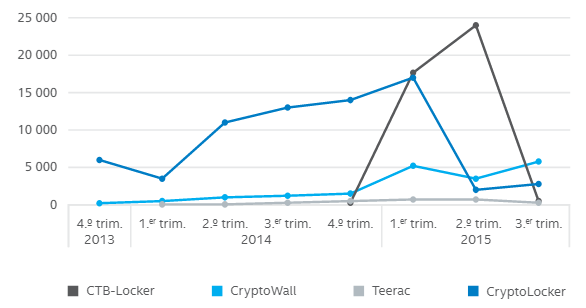
\includegraphics{ransomware}
	\caption{Nuevas muestras de familias de ransomware prominentes \cite{mcafee-predictions}}
	\label{fig:ransomware}
\end{figure}

Podemos encontrar incluso ejemplos relativamente recientes como puede ser \textit{WannaCry}, ransomware que afecto hace no mucho a decenas de países inutilizando sistemas de diversa índole, desde la Intranet de Telefónica hasta varios hospitales en Reino Unido \cite{wannacry1} \cite{wannacry2}.


\subsection{Rootkits}

Los rootkits son una clase de malware que tiene como objetivo principal escalar privilegios en el sistema, también conocido como conseguir acceso de superusuario o \textit{root}. No hace falta mencionar que con dichos privilegios el daño que puede causar en un sistema es inconmensurable, pudiendo dejarlo completamente inutilizado o eliminar absolutamente toda su información.

\subsection{RATs}

Los \textit{Remote Administration Tools} también conocidos como RAT, buscan ofrecer a los posibles atacantes una puerta trasera para acceder a los sistemas para así poder introducir otros tipos de malware específicos.

\subsection{Spyware}

Un tipo de malware concreto bastante popular desde la década del 2000 es el denominado spyware, cuyo objetivo es obtener información de las acciones de un sistema, infectando la máquina destino de manera inadvertida para el usuario, el cual desconoce que su actividad y/o sus datos están siendo monitorizados.

\subsection{Keyloggers}

El \textit{Keystroke Logger}, mejor conocido como Keylogger, es otro tipo de malware usado actualmente debido a su efectividad cuyo objetivo consiste en obtener la información de las pulsaciones que se realizan en un teclado de un sistema concreto. Este mecanismo tiene como principal objetivo extraer información, especialmente contraseñas, de un usuario para después poder acceder a los servicios que usa dicho usuario. Se puede encontrar Keyloggers tanto a nivel físico, en forma de pequeños dispositivos\footnote{\url{https://www.keelog.com/}} USB con una memoria interna\footnote{\url{https://store.hackaday.com/products/usb-rubber-ducky-deluxe}}, como a nivel de software, estos últimos especialmente sencillos de implementar con solo unas pocas lineas de código \cite{ander-keylogger}.

%------------------------------------------------------------------------------

\section{Dispositivos móviles}

El malware afecta a los sistemas y es un riesgo para la seguridad de estos, pero no es el único. Además hay que tener en cuenta que en los últimos años el mundo de las tecnologías de la información ha sufrido cambios drásticos. Lejas queda el modelo clásico de ordenadores personales y servidores estándar que conforman Internet. Han entrado a la palestra nuevas áreas que se han ido desarrollando durante los últimos años. A medida que estas áreas han ido destacando, el campo de la seguridad informática ha ido avanzando para satisfacer las necesidades de seguridad de estas áreas y adaptarse a ellas mediante nuevas técnicas y medidas de seguridad.

Una de las áreas que ha destacado estos últimos años es el área de la seguridad de dispositivos móviles. Datos como que el consumo de Internet a día de hoy es mayor en este tipo de dispositivos que en ordenadores convencionales resultan sorprendentes. En el caso concreto de España, del 78,7\% de la población que se conecta regularmente a Internet, el 88,3\% de los usuarios lo hace a través de un smartphone \cite{smartphones-internet}. Teniendo eso en cuenta, es lógico que la seguridad estos dispositivos sea una prioridad y a su vez uno de los puntos de enfoque por parte de todo tipo de atacantes.

Los smartphones tienen una gran cantidad de usos diferentes. Aparte de ser la principal herramienta de comunicación, también son dispositivos mediante los que se procesa una gran cantidad de información, desde información personal como fotos o mensajes a información relacionada con el ámbito empresarial como documentos o correos. Debido a que la información ya no solo se procesa y transmite desde ordenadores tradicionales, sino que en su mayoría se hace desde dispositivos móviles, resulta necesario definir e implantar técnicas y procedimientos de seguridad en este tipo de dispositivos.

\subsection{Seguridad en smartphones}

Aunque en esencia los smartphones se traten de dispositivos basados en Linux, Unix o derivados, este tipo de dispositivos tienen sus particularidades con respecto a los ordenadores personales. Primeramente, estos sistemas no disponen de la arquitectura x86/x86-64 (al menos en su gran mayoría), sino que se basan en procesadores con arquitectura ARM. Debido a esto y al enfoque de uso que tienen, usan diferentes sistemas operativos que distan de los tradicionales. Los sistemas operativos más usados para smartphones son Android e iOS, que se encuentran en un 86,22\% y 12,88\% de los dispositivos vendidos en 2016 \cite{gartner-uso-so}, respectivamente.

Ambos son sistemas que, al estar por defecto más limitados en uso y configuración, resultan \textit{a priori} más seguros que los sistemas operativos de escritorio. Existen una serie de técnicas que se suelen aplicar independientemente del sistema operativo utilizado, como pueden ser la firma de aplicaciones o el uso de cifrado para ciertos casos. Aun así, este tipo de medidas son prácticamente obligatorias para disponer de sistemas mínimamente seguros. Lo que diferencia a cada uno de los sistemas operativos desde el punto de vista de la seguridad es tanto el enfoque de seguridad que le dan al sistema como las técnicas, medidas, arquitecturas de software o algoritmos, que cambian de un sistema operativo a otro.

\subsubsection{Seguridad en iOS}

En dispositivos con iOS la seguridad se enfoca desde varios puntos. Uno de los puntos en los que iOS destaca es en su tienda de aplicaciones, la \textit{App Store}, que dispone de ciertos filtros y controles de seguridad a la hora de publicar aplicaciones con el objetivo de dificultar en la mayor medida posible que a través de las aplicaciones entre algún tipo de malware.

Por otro lado, uno de los puntos más fuertes de iOS es el relacionado con en el cifrado. Debido a la ventaja que otorga el hecho de que la misma compañía elabore tanto el hardware como las diferentes capas de software de sus dispositivos, se pueden integrar medidas de seguridad en el propio hardware que funcionen de manera conjunta a su software. Una de las más destacables es la incorporación del coprocesador llamado \emph{Secure Enclave} \cite{ios-sec-guide}. Este coprocesador (disponible en el Apple S2, y en el Apple A7 y posteriores) se encarga de todas las operaciones criptográficas para la gestión de claves de cifrado de datos y mantiene la integridad de la protección de datos, incluso si el kernel del sistema se ha visto comprometido. Usa memoria cifrada e incluye un generador aleatorio de números por hardware. La comunicación entre este coprocesador y el procesador principal esta completamente aislada del resto del sistema.

Esto tiene dos ventajas. La primera, que el cifrado por hardware, al realizarse de manera transparente a cualquier capa de software, resulta díficilmente evitable. Por otra parte, a nivel de rendimiento, resulta mucho más eficiente que cualquier tipo de cifrado por software.

Además, todos los dispositivos iOS tienen un sistema de cifrado mediante hardware y AES-256 que se sitúa entre la memoria principal y el almacenamiento flash \cite{ios-sec-guide}, de tal manera que los datos almacenados en los dispositivos se mantienen cifrados sin que se pierda rendimiento en ello. Para cada sistema de cifrado se crea identificadores únicos tanto par cada usuario (UID) como para cada grupo distinto de dispositivos (GID), ambos integrados en el propio hardware. Cada UID es único y no es conocido ni por Apple ni por ninguna aplicación ni usuario. Cada GID es común a una familia de dispositivos y se usa para distinguirlos entre sí. Esto hace que los datos que se almacenan sean altamente difíciles de descifrar.

Las operaciones de cifrado y descifrado concretas siguen el esquema que se muestra en la Figura \ref{fig:ios-data-encrypt} , haciendo uso también de una contraseña propia elegida por el usuario, la que se muestra en el diagrama con el nombre de \textit{Passcode Key}.

\begin{figure}[H]
	\centering
	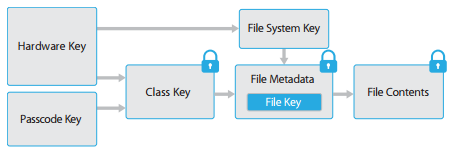
\includegraphics{ios-data-encrypt}
	\caption{Esquema de cifrado de un archivo en iOS}
	\label{fig:ios-data-encrypt}
\end{figure}

\subsubsection{Seguridad en Android}

El modelo de seguridad en Android se diferencia del modelo de iOS en varios aspectos. Más que en un fuerte cifrado a todos los niveles, el cual también usa pero en menor medida, el enfoque se basa en hacer lo más segura posible cada aplicación. Esto es lógico teniendo en cuenta que, por un lado, la tienda de aplicaciones de Android, la \textit{Play Store}\footnote{\url{https://play.google.com/store/apps}}, es menos estricta que la de iOS y que, por otro lado, Google (propietaria de Android) no fabrica los dispositivos que integran dicho sistema. Por ello, la arquitectura de software del sistema resulta más jerárquica, y es fundamental para las diversas medidas de seguridad que se implementan. En la Figura \ref{fig:android-arch} se muestran las diferentes capas de dicha arquitectura. 

\begin{figure}[H]
	\centering
	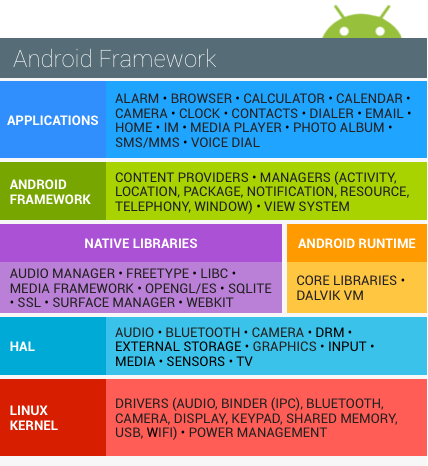
\includegraphics{android-arch}
	\caption{Las diferentes capas que componen la arquitectura de Android}
	\label{fig:android-arch}
\end{figure}

La esencia de la seguridad en Android reside en controlar y limitar la interacción entre las diferentes capas para evitar fallos de seguridad. Para ello se hace uso de diferentes técnicas \cite{android-sec-guide} \cite{jspdcp-2014} como:

\begin{itemize}
	\item El \emph{sandboxing}, donde el código de cada aplicación se ejecuta de manera aislada al resto de aplicaciones y, además, los datos de cada aplicación se mantienen separados. 
	\item Un framework de aplicaciones que implementa ciertas técnicas comunes de seguridad como, por ejemplo, métodos criptográficos, sistemas de permisos o una comunicación entre procesos (\textit{IPC, Interprocess Communication}) segura.	
	\item Implementar diversas tecnologías como ASLR (\textit{Address Space Layout Randomization}), NX (\textit{No-eXecute}), \textit{ProPolice}, \textit{safe\textunderscore iop, OpenBSD dlmalloc}, \textit{OpenBSD calloc}, y \textit{Linux mmap\textunderscore min\textunderscore addr} para evitar errores de \textit{buffer overflow}, para evitar que se ejecuten instrucciones concretas o para mitigar otro tipo de riesgos relacionados con la gestión de la memoria.
	\item Un sistema de cifrado de archivos mediante AES-256 para proteger los datos almacenados en los dispositivos.
	\item Un sistema de permisos tanto a nivel de usuario como al nivel de cada aplicación concreta para controlar las acciones de los usuarios y las aplicaciones.
\end{itemize}

Este enfoque hace que, por una parte, el propio Android mediante su arquitectura y el uso de una VM (Virtual Machine) específicamente creada para el sistema (como se puede observar en la Figura \ref{fig:android-arch}) ofrezca un repertorio de mecanismos de seguridad que hacen de él un sistema relativamente seguro. Por otra parte, también pone empeño en que los desarrolladores tienen la necesidad de implementar medidas de seguridad en sus aplicaciones para garantizar la seguridad de las mismas. Para ello, el SDK de Android proporciona acceso a un gran número de utilidades como, entre otras, utilidades de cifrado, de manejo de credenciales o de intercambio de mensajes.

%------------------------------------------------------------------------------

\section{Internet of Things}

También junto a la seguridad de los dispositivos móviles, que viene determinada por el auge de dichos dispositivos, el área de la seguridad del Internet of Things (conocida como IoT) es una de las áreas que más impulso está teniendo, debido al mismo motivo. Cada vez hay una mayor cantidad de dispositivos conectados a Internet, que no ha hecho más que crecer exponencialmente debido al IoT. Dispositivos que ya no se tratan exclusivamente de móviles, tablets u ordenadores, sino de otro tipo de dispositivos, como electrodomésticos o automóviles, que han sido dotados de capacidad de computación y conexión a Internet para ampliar sus capacidades y poder recopilar información de ellos. En esencia, el IoT se basa en una serie de dispositivos a los que, mediante el uso de sensores, procesadores y conexión a Internet, se les da la capacidad de recoger y transmitir información a otros dispositivos, además de recibir dicha información para actuar de una manera u otra.

\subsection{Aplicaciones}

Las aplicaciones de lo que se denomina Internet of Things son diversas y variadas. Prácticamente cualquier sistema electrónico que disponga de una serie de sensores mediante los cuales obtenga información puede ver multiplicadas sus capacidades añadiéndole una conexión a la red. De esta manera se le dota de capacidad para ya no solo transmitir información sino incluso poder interactuar de forma más compleja con otra serie de sistemas \cite{Miorandi20121497} \cite{Gubbi20131645}.
	
\subsubsection{Smart homes}

Mediante tecnologías IoT se puede dotar a los diferentes elementos domóticos de un hogar o edificio de capacidades para reaccionar de manera automática a diferentes cambios que se puedan dar. Desde controlar la luz o el agua hasta controlar la temperatura o las persianas, todo de tal manera que los subsistemas sean capaces de comunicarse y actuar de manera conjunta en función de la información que reciben.
	
\subsubsection{Smart Cities}

El término Smart Cities se refiere al sistema ciberfísico que conforma una red avanzada de comunicación para optimizar el uso de los sistemas físicos de una ciudad. Puede optimizar servicios como por ejemplo el tendido eléctrico, mediante el análisis de consumo de toda la red eléctrica, o la red de carreteras, mediante sistemas avanzados de control de tráfico (del cual los vehículos autónomos se pueden beneficiar). Esos son solo unos breves ejemplos de lo que un sistema de este tipo puede llegar a optimizar dentro de los procesos que se dan en una ciudad.
	
\subsubsection{Monitorización medioambiental}

El IoT también puede servir para monitorizar cambios en el medio ambiente e integrar todo esa adquisición de datos para que funcione de manera conjunta con otros sistemas. Una serie de sistemas de tiempo real, a los que se añade la capacidad de comunicarse e interactuar entre sí, pueden ser una plataforma sólida mediante la cual detectar y monitorizar anomalías que afecten a la vida humana, animal y vegetal. Además, pueden ser una herramienta fundamental para obtener información que permita mitigar los efectos de cualquier tipo de contaminación medioambiental.
	
\subsubsection{Sanidad}

La sanidad también es uno de esos sectores que se puede beneficiar de los avances en el IoT. Por ejemplo, la capacidad para monitorizar diferentes parámetros (como la temperatura corporal, la presión sanguínea o la actividad cardíaca) de manera constante puede ser una herramienta fundamental a la hora de prevenir y tratar diversas enfermedades. Además del nivel patológico, se pueden usar diferentes dispositivos para tomar información que permita mejorar el estilo de vida y la salud de las personas. Dispositivos como los wearables son un buen ejemplo de ello, entre los que se encuentran las famosas pulseras cuantificadoras. 
	
\subsubsection{Smart Business}

El término Smart Business hace referencia a todas esas aplicaciones del Internet of Things que se usan para mejorar tanto la logística interna como los productos y servicios que ofrece una empresa o negocio. La gestión de inventario en tiempo real o la automatización del envío de información sobre productos para ofrecer un mejor servicio post venta son dos ejemplos en los que enfatizan cada vez mas empresas.
	
\subsubsection{Seguridad y vigilancia}

Aunque pueda ser polémico, el Internet of Things también se puede aplicar en el área de la seguridad y vigilancia. Los sistemas interconectados de cámaras o los sensores para detectar químicos nocivos son dos ejemplos. El primero de ellos no se respeta la privacidad del usuario, mientras que el segundo sí. Debido a eso, aplicaciones como la primera son objeto de numerosas críticas por parte de diversas organizaciones.

\subsection{Seguridad en Internet of Things}

Uno de los principales problemas del Internet of Things reside en que ya no solo se trata de el peligro de que la información se vea comprometida o revelada sino que, al tratarse de otra serie de dispositivos, los peligros son mucho mayores \cite{iot-qz}\cite{iot-techradar}. Esto es algo de lo que el mundo de la seguridad informática ya se ha percatado. Estimando que el número de dispositivos conectados a Internet pasará de 6,4 mil millones en 2016 a 21 mil millones en 2020 \cite{iot-searchdatacenter} debido al auge del IoT, resulta fundamental indagar en ello. 

En la actualidad existen gran cantidad de casos en los que diferentes dispositivos salen al mercado con esas capacidades para conectarse a Internet pero que carecen de prácticamente ningún tipo de medida de seguridad. Se han dado casos como el de Miele \cite{iot-miele} donde a causa de la falta de seguridad en un modelo de sus lavavajillas, se puede llegar a acceder a la red local privada a donde este conectado de manera sencilla. Otro caso es el de los automóviles Tesla \cite{iot-tesla}, donde más de una vez se han descubierto vulnerabilidades que permiten obtener el control total de sus vehículos y conducirlos remotamente a placer del atacante. Esto es gravísimo, pudiendo llegar a poner en en riesgo la vida de personas. Por ello, los servicios de la seguridad informática son mas necesarios si cabe para este campo. 

%------------------------------------------------------------------------------

\section{Cloud Computing}

El Instituto Nacional de Estándares y Tecnologías de Estados Unidos, conocido como NIST (\textit{National Institute of Standards and Technologies}) define el Cloud Computing como:

\begin{quotation}
\textit{''Un modelo para hacer posible el acceso a red adecuado y bajo demanda a un conjunto de recursos de computación configurables y compartidos (por ejemplo, redes, servidores, almacenamiento, aplicaciones y servicios…) cuyo aprovisionamiento y liberación puede realizarse con rapidez y con un mínimo esfuerzo de gestión e interacción por parte del proveedor de dicha nube''.} \cite{inteco-cloud}
\end{quotation}

En esencia, podemos entender como Cloud Computing a una extensión de las aplicaciones de Internet, que eran principalmente aplicaciones web y transmisión de datos, a nuevas posibilidades, entre las cuales se incluyen plataformas completas y software más complejo, ofrecidas como un modelo de servicio configurable y escalable.

Las estructuras cloud se pueden clasificar en tres categorías: públicas, comunitarias y privadas. En las primeras el acceso a sus servicios es abierto, mientras que en las segundas está acotado a un determinado entorno, normalmente una empresa. En la última, aunque no se tiene acceso público a sus servicios, estos se comparten entre varias entidades.

\subsection{Tipos de servicios}

El Cloud Computing puede ofrecer una serie de servicios a sus usuarios, y en función de qué servicio se ofrezca, se clasifica en una de las tres categorías diferentes existentes que se mencionan a continuación.

\subsubsection{Software as a Service}

\emph{Software as a Service} consiste en un despliegue de software en el cual las aplicaciones y los recursos computacionales se han diseñado para ser ofrecidos como servicios de funcionamiento bajo demanda. De esta forma se reducen los costes tanto de software como hardware, así como los gastos de mantenimiento y operación. En esta categoría las consideraciones sobre seguridad son responsabilidad del proveedor del servicio, estando limitada la configuración que puede realizar el suscriptor.

\subsubsection{Platform as a Service}

\emph{Platform as a Service} es el servicio donde se ofrece una plataforma en la cual el suscriptor del servicio puede desplegar su propio software. Con ello se reducen los costes y la complejidad de la compra, el mantenimiento, el almacenamiento y el control del hardware y el software que componen la plataforma. El suscriptor del servicio tiene un control total sobre las aplicaciones y un control parcial de la configuración del entorno ya que la instalación de los entornos dependerá de la infraestructura que el proveedor del servicio haya desplegado. La seguridad se comparte entre el proveedor del servicio y el suscriptor ya que el suscriptor aporta su propio software.

\subsubsection{Infrastructure as a Service}

\emph{Infrastructure as a Service} es un modelo en el cual la infraestructura (servidores, software y equipamiento de red) es gestionada por el proveedor como un servicio bajo demanda, en el cual se pueden crear entornos para desarrollar, ejecutar o probar aplicaciones, El fin principal de este modelo es evitar la compra de recursos por parte de los suscriptores, ya que el proveedor ofrece estos recursos como objetos virtuales accesibles a través de un interfaz de servicio. El suscriptor mantiene generalmente la capacidad de decisión del sistema operativo y del entorno que instala. Por lo tanto, la gestión de la seguridad corre principalmente a cargo del suscriptor.

\subsection{Seguridad en Cloud Computing}

Debido al auge del Cloud Computing surge la CSA (\textit{Cloud Security Alliance}). La CSA se define como una organización internacional sin ánimo de lucro que tiene como objetivo promover el uso de una serie de buenas prácticas para garantizar la seguridad en la nube.
Entre otras actividades, la CSA elabora un informe periódico con las mayores amenazas de seguridad de sistemas de Cloud Computing \cite{csa-cloud-12-threats}. Estas amenazas se actualizan regularmente buscando el consenso de los expertos. A continuación, se resumen las amenazas descritas en este informe. En el informe de 2016, la CSA marca como amenazas más graves, ordenadas por orden de importancia, los siguientes 12 puntos:
\begin{enumerate}
	\item Brechas de Datos
	\item Manejo inseguro de Credenciales de Acceso
	\item Interfaces y APIs inseguros
	\item Vulnerabilidades de Sistemas y Aplicaciones
	\item Secuestro de Cuentas
	\item Amenazas Internas
	\item Advanced Persistent Threats (APTs)
	\item Pérdida de Datos
	\item Diligencia insuficiente
	\item Abuso y mal uso del Cloud Computing
	\item Denegación de Servicio
	\item Problemas derivados de las tecnologías compartidas
\end{enumerate}

Con el auge del Cloud Computing, este tipo de amenazas son cada vez más graves. Desde servicios de almacenamiento de datos hasta plataformas de despliegue de aplicaciones, cada vez más empresas y usuarios delegan almacenamiento, infraestructura, o software en servicios de Cloud Computing, por lo que, en primer lugar, ser conscientes de la ventajas, inconvenientes y, sobre todo, riesgos que acarrea el uso de estos servicios resulta fundamental para después, en segundo lugar, ser capaces de securizarlos en la mayor medida posible y hacer un uso seguro de esto servicios.
\chapter{Pentesting}

\epigraph{\textit{''Si piensas que la tecnología puede solucionar tus problemas de seguridad, está claro que ni entiendes los problemas ni entiendes la tecnología''}}{--- Bruce Schneier}

Dentro de la seguridad informática un test de intrusión, o \textit{pentesting}, como se conoce en inglés, evalúa los diferentes niveles de seguridad de un sistema informático red mediante la simulación en un entorno controlado de un ataque por parte de un usuario malicioso conocido comúnmente como hacker \cite{pentesting-kali}. El propósito de una prueba de penetración es determinar la viabilidad de un ataque y la cantidad de impacto que puede causar este mismo.

\section{Objetivos}

A día de hoy el pentesting es una de las técnicas más utilizadas para garantizar tanto la seguridad de la información como la propia seguridad informática de los sistemas de empresas u organizaciones. Es uno de los pilares básicos en las auditorías de seguridad informática, en las que empresas contratan a expertos en seguridad para evaluar la fortaleza de sus sistemas informáticos.

El pentesting no es un área con unas técnicas de actuación concretas. El pentesting usa una grandísima cantidad de técnicas, a las cuales se van añadiendo técnicas que van surgiendo, para determinar la seguridad de un sistema informático y, en particular, conocer las debilidades que tiene el sistema informático.

Haciendo un símil con otras áreas completamente diferentes, un pentesting podría equivaler a una serie de pruebas prácticas que se realizan, por ejemplo, en controles de calidad para todo tipo de productos, en los cuales se ve que la mejor forma de probar el correcto funcionamiento de dichos productos consiste en someterlos a una serie de pruebas. Dichas pruebas están basadas en los entornos reales en los que se utilizan esos productos.

Por ejemplo: la mejor manera de probar la efectividad de un chaleco antibalas es realizando disparos sobre él para ver hasta qué punto los materiales como el Kevlar o de los tejidos que han sido compuestos para dicho chaleco son adecuados para parar una bala. De la misma manera, la mejor forma de probar si un sistema informático o una red compuesta de varios sistemas es segura, o mejor dicho, hasta qué punto es segura, es elaborar ciertas pruebas e intentar explotar vulnerabilidades que puedan surgir en estos sistemas. Todo ello con el objetivo final de sacar conclusiones y, en base a esas conclusiones, mejorar y fortificar ese sistema.

Aunque, de la misma manera que jamás se harían pruebas con el chaleco antibalas comprometiendo la integridad de ninguna persona física, tampoco se elabora un pentesting comprometiendo de manera real ningún sistema. El pentesting, al igual que las pruebas del chaleco, se elaboran ambas en un entorno controlado y limitado.

Teniendo en cuenta que la seguridad de los sistemas informáticos es vital para la continuidad del negocio y el correcto desarrollo de las actividades de una empresa u organización, y siendo el pentesting una de las mejores herramientas para garantizar dicha seguridad, resulta lógico que este sea uno de los métodos más usados por todo tipo de empresas u organizaciones.


%------------------------------------------------------------------------------

\section{Partes}

Dentro de un pentesting se diferencian una serie de etapas, cada una de las cuales tiene objetivos particulares y concretos. Aunque algunas de estas partes puedan tener sentido de manera independiente, en su conjunto permiten un completo análisis de un sistema informático del cual sacar conclusiones que permitan preservar la seguridad.

A continuación, se enumeran y definen las fases de un test de intrusión o pentesting, que ya se encuentran estandarizadas en el PTES (\textit{Penetration Testing Execution Standard}) \cite{ptes}:

\begin{figure}[H]
	\centering
	
\includegraphics[width=150px]{ptes}
	\caption{Logo de Penetration Testing Execution Standard}
	\label{fig:ptes}
\end{figure}

\begin{enumerate}
	\item \textbf{Reglas del juego, alcance y términos del test de intrusión:} en esta fase se establece una serie de protocolos entre el realizador del pentesting (normalmente una auditoría de seguridad informática) y el auditado (normalmente una empresa u organización). En esta fase se establecen los objetivos a los que llegar, los límites a los que tendrán que adherirse los auditores.
	\item \textbf{Recolección de información:} fase en la que se obtiene información del sistema para enfocar posteriormente analizarla.
	\item \textbf{Análisis de las vulnerabilidades:} fase en la que mediante la información obtenida, se pasa a determinar las vulnerabilidades del sistema.
	\item \textbf{Explotación de las vulnerabilidades:} tras determinar esas vulnerabilidades, se pasa a intentar explotarlas para visualizar su gravedad y el daño real que pueden causar.
	\item \textbf{Postexplotación del sistema:} tras haber logrado explotar una vulnerabilidad, se intenta minar lo más posible el sistema, intentando lograr un efecto en cadena para ver, hasta qué punto, se puede dañar un sistema mediante una vulnerabilidad concreta.
	\item \textbf{Generación de informes:} tras todos los pasos anteriores, se condensa todo el proceso elaborado y las conclusiones a las que se ha llegado en informes, de tal manera que a través de esos informes, se pueda actuar para corregir las vulnerabilidades y fortalecer el sistema.
\end{enumerate}

De todas esas fases, a continuación se profundizará en las más importantes.

\section{Recogida de información}

\textit{''La información es poder''}. Esa frase, atribuida a Francis Bacon (aunque se desconoce si realmente llegó a pronunciarla en algún momento), no podría ser más cierta actualmente. La informática no es más que la ciencia que trata la información, y la seguridad informática es un área que se encarga de protegerla. Por ello, a la hora de realizar un pentesting, resulta esencial obtener la mayor cantidad de información posible. El éxito de muchos de los ataques e intrusiones que sufren empresas y organizaciones se debe en gran parte a la gran cantidad de información que directa e indirectamente un atacante es capaz de obtener sobre sus sistemas \cite{inteco-gathering}.

Por ello, la fase de recogida de información o \textit{Information Gathering} resulta fundamental a la hora de realizar un test de intrusión. A mayor cantidad de información obtiene un atacante de un sistema mayor probabilidad de éxito tendrá al atacar.

La recogida de información, según desde qué punto se realiza, se puede separar en dos categorías: \textit{External Footprinting} e \textit{Internal Footprinting}. La primera hace referencia obtener información desde fuera del sistema y la segunda obtener información dentro del sistema.

\subsection{Internal Footprinting}

El Internal Footprinting engloba toda la recogida de información que se realiza una vez se tiene acceso, parcial o completo, al sistema o la red de la que se desea obtener la información. Este tipo de recogida de información no se realiza en la segunda fase de un pentesting, es decir, al comienzo del pentesting, sino que se realiza en la fase de post explotación del sistema, la quinta fase de un test de intrusión. Es lógico que, sin todavía haber explotado ninguna vulnerabilidad, y por ende todavía no se haya accedido al sistema, no se pueda recoger información dentro de él.

\subsection{External Footprinting}

El External Footprinting engloba toda la recogida información, que al contrario que en el Internal Footprinting, se realiza desde fuera del sistema. Este tipo de recogida información sí que se realiza en la segunda fase de un test de intrusión, y de hecho es el primer paso esencial a realizar. A través de diversas técnicas se busca obtener la mayor cantidad de información posible de una red o un sistema para, posteriormente, analizarla y encontrar vulnerabilidades.

Las técnicas de recogida de información englobadas dentro del External Footprinting se pueden dividir a su vez en dos subcategorías, en función del grado de agresividad de las mismas. 

\subsubsection{Active Footprinting}

Por un lado, está el descubrimiento activo, denominado Active Footprinting, que destaca por interactuar directamente con la infraestructura del sistema objetivo mediante consultas al DNS, análisis de las cabeceras HTTP, enumeración de puertos y sus servicios, etcétera \cite{pentesting-kali}. Seguidamente se explicarán brevemente en qué consisten algunas de estas técnicas, sin la intención de entrar en las herramientas de software concretas.

\paragraph{Escaneos DNS}

Una de las formas más comunes a la hora de obtener información consiste en obtener información de los servidores DNS. DNS (Domain Name Services) es un protocolo que permite la conversión entre direcciones de red numéricas, como son las IPs, y direcciones FQDN (Full Qualified Domain Name), que son direcciones del estilo \url{miweb.es}. De esta manera, DNS provee una capa de abstracción para hacer más sencillo las conexiones por parte de los usuarios y administradores a otros servicios.

La transformación de una dirección IP en un nombre de dominio se conoce como resolución DNS, y su proceso inverso (de nombre de dominio a IP) se conoce como resolución inversa. Este tipo de operaciones se da en los servidores DNS, de los cuales, mediante diferentes técnicas se puede extraer información relevante, hasta tal punto que se puede llegar a determinar ciertos aspectos de la topología de la red en la que se encuentra el sistema al que estamos intentando acceder.

\paragraph{Fingerprinting}

El Fingerprinting consiste en obtener información del propio sistema al que se intenta acceder. Datos como el sistema operativo y su versión o las aplicaciones que usa son esenciales a la hora de buscar vulnerabilidades que se puedan explotar en el sistema para lograr acceso a este, aunque no se limita solo a este tipo de datos. Obtener el servidor web que usa determinado dominio o el CMS (\textit{Content Management System}) que usa dicho servidor web es fundamental a la hora de determinar vulnerabilidades concretas para dicho software. Existen herramientas tanto para obtener esta información como para relacionarla con bases de datos, previamente elaboradas, en las que se encuentran gran cantidad de vulnerabilidades que ya han sido detectadas.

\paragraph{SMTP}

Otra de las áreas mediante las que se puede obtener información es la relacionada con el protocolo SMTP. Con ello se puede obtener desde información de los dominios de correo electrónico usados hasta direcciones de correo electrónicas concretas, lo que permite centrarse en vulnerabilidades para dichos dominios. Esto deriva en que se pueda lograr suplantar la identidad de cierto usuario.

\subsubsection{Passive Footprinting}

Por otro lado se encuentra el descubrimiento pasivo, lógicamente denominado Passive Footprinting, que recurre a la consulta de la información previamente indexada por motores de búsqueda, registros públicos, foros, etcétera, por lo que no interactúa directamente con el sistema a penetrar \cite{pentesting-kali}. 

\paragraph{Whois}

Whois es un protocolo TCP que permite obtener datos sobre el propietario de un nombre de dominio o una dirección IP. Entre los datos que se pueden obtener, se encuentran el correo electrónico, el nombre completo, la ciudad, el código postal o el número de teléfono del propietario. Estos datos son de fácil acceso, existiendo incluso herramientas web que te permiten obtener dicha información mediante el mencionado protocolo.

\paragraph{Hacking con buscadores}

Los buscadores como Google o Bing son utilizados por la gran mayoría para encontrar sitios web. Lo que no todo el mundo conoce es que se tratan de una poderosísima herramienta para obtener información adicional sobre uno o varios sitios web. La gran mayoría de buscadores disponen de parámetros avanzados de búsqueda que permiten buscar palabras concretas en las URLs, buscar por una determinada extensión o buscar dentro un sitio web concreto. De esta forma, si se sabe qué buscar, se puede obtener información sobre qué vulnerabilidades se pueden explotar en cierta página web.

Aparte de los buscadores tradicionales, también existen una serie de buscadores especializados en la búsqueda de dispositivos, enfocados al IoT, en los que se pueden buscar desde webcams hasta electrodomésticos, con la condición de que estén conectados a Internet. Estos buscadores, como Shodan\footnote{https://www.shodan.io/}, permite también filtrar búsquedas y realizar búsquedas avanzadas que permitan obtener información sobre otros sistemas que no sean directamente servidores web.

\paragraph{Social network engineering}

La ingeniería social, aunque no dispone de herramientas concretas, son técnicas para obtener información a partir de las redes sociales. En las redes sociales, muchas veces de manera inconsciente o sin comprender las consecuencias que puede acarrear, se comparte una gran cantidad de información personal que, bien analizada, puede ser determinante para elaborar un ataque concreto.

\section{Análisis de vulnerabilidades}

Una vez obtenida toda la información posible sobre el sistema, se pasa a la siguiente fase definida en el PTES, que consiste en analizar qué vulnerabilidades concretas se pueden explotar. La información recogida se usa para obtener como resultado final un listado de vulnerabilidades que se pueden llegar a explotar en el sistema. Esta fase de análisis pasa por tres periodos.

\subsection{Pruebas}

En el primer periodo se realiza una serie de pruebas basándose en la información que disponemos del sistema, que previamente hemos obtenido. La información que nos den estas pruebas es importante, cuanto mayor número de pruebas se realicen mediante el mayor número de herramientas y técnicas posible los resultados mejorarán. Estas pruebas se engloban en pruebas pasivas o activas.

\subsubsection{Activas}

Las pruebas activas requieren interactuar directamente con el componente a auditar. Tienen una estrecha relación con el Active Footprinting, ya que se basan en la información obtenida de esa manera. Dentro de éstas se incluyen las siguientes categorías:

\begin{itemize}
	\item \textbf{Automatizadas:} mediante diversas herramientas de software se interactúa con el sistema, enviando peticiones, escaneando los servicios, etc.
	\item \textbf{Conexión manual:} para evitar falsos positivos que puedan dar las pruebas automatizadas, se llevan a cabo pruebas manuales, que realizan los mismos pasos que las automáticas pero sin el uso de dichas herramientas de análisis de vulnerabilidades.
	\item \textbf{Ofuscadas:} con el objetivo de evitar la detección o el bloqueo por parte de sistemas IDS (\textit{Intrusión Detection System}), IPS (\textit{Intrusion Prevention System}) o WAF (\textit{Web Application Firewall}), se realizan pruebas que se comportan de diferente manera a las pruebas tradicionales, alargando tiempos de espera entre peticiones, modificando ciertos aspectos de las peticiones o alternando entre objetivos.
\end{itemize}

\subsubsection{Pasivas}

La pruebas pasivas consisten en analizar la información obtenida mediante Passive Footprinting. Analizar dicha información puede permitirnos suponer la existencia de cierta vulnerabilidad en el sistema. A diferencia de las pruebas activas, estas contienen un mayor componente subjetivo y abstracto.

\subsection{Validación}

Una vez elaboradas una serie de pruebas necesitamos correlar la información que nos ha dado esa serie de pruebas. En este paso, el objetivo es enmarcar la vulnerabilidad encontrada en un apartado técnico, clasificándola en una serie de categorías e indentificándola de una manera concreta. Esta clasificación se puede realizar a varios niveles.
El más concreto consiste en identificarlas mediante, valga la redundancia, identificadores concretos como el CVE\footnote{https://cve.mitre.org/} (\textit{Common Vulnerabilities and Exposures}). También se puede hacer a un nivel más global, mediante las categorías marcadas en diversas normas, como pueden ser el \emph{NIST SP 800-53}\footnote{https://nvd.nist.gov/800-53} o la \textit{Guía OWASP}\footnote{https://www.owasp.org/}.
	
\subsection{Investigación}

Tras la identificación de una vulnerabilidad, y haberla categorizado correctamente, es necesario evaluar la gravedad de dicha vulnerabilidad. Para ello se procede a realizar una investigación sobre dicha vulnerabilidad. Esta investigación puede ser privada, elaborando pruebas a nivel interno, como ataques de fuerza bruta o configurar replicas del entorno mediante el uso de máquinas virtuales (VM) para emular el entorno real y hacer pruebas con ello.

\section[Explotación de vulnerabilidades]{Explotación de vulnerabilidades: Ataques de penetración}

En las dos secciones anteriores se ha explicado la recogida y el análisis de la información, respectivamente. La sucesión de esas dos fases tienen como objetivo final explotar una serie de vulnerabilidades. En ello reside la esencia del pentesting, penetrar en un sistema mediante la explotación de dichas vulnerabilidades, realizando una serie de ataques a estos. Dependiendo del tipo de ataque, la vulnerabilidad que se explota o el objetivo del ataque, se pueden clasificar en prácticamente una infinidad de categorías. En los siguientes puntos se explican algunas de ellas, que se consideran entre las más importantes.

\subsection{Ataques de contraseñas}
La contraseñas son un mecanismo de sobra conocido, que se remonta a mucho antes de la invención de la informática e incluso son anteriores a la propia formalización de la lógica que cimienta todo el desarrollo de la informática y la electrónica digital. Si desde la antigüedad se llevan usando las contraseñas para limitar el acceso solo a ciertas personas a ciertos sitios, en la actualidad se usan para limitar el acceso por parte de cierto usuario a cierto sistema o servicio informático. A día de hoy son, aun con el auge de métodos biométricos, la herramienta de control de acceso más usada.

Partiendo de esa base, los ataques de contraseñas son cualquier técnica o mecanismo orientados a descifrar o romper las contraseñas usadas para proteger esos sistemas. Cabe destacar que todo mecanismo de autenticación por contraseñas se basa en la comparación de \emph{hashes} y no en la comparación de contraseñas, dando autorización solo cuando el hash de la contraseña introducida coincide con el almacenado previamente, que ha sido generado con anterioridad mediante la contraseña elegida para la protección de ese sistema.

Un \emph{hash} no es más que una cadena alfanumérica de longitud fija, la cual se genera en base a una \emph{función hash}. La esencia de esas funciones radica en que generar un hash es sencillo y poco costoso, pero obtener la cadena original (es decir, la contraseña) mediante el hash es extremadamente complicado, aunque dicha complejidad depende del algoritmo usado. Ejemplos de dichos algoritmos son SHA-1 o MD5.

\subsubsection{Fuerza bruta}

Lo ataques de contraseñas se pueden elaborar de varias maneras. El método mas básico es el de fuerza bruta, que como su nombre indica, consiste en probar todas las combinaciones posibles de contraseñas. Esto puede ser especialmente costoso a nivel computacional. En las Tablas \ref{table:contrasenas} y \ref{table:contrasenas-explotar} se puede ver la cantidad de contraseñas posibles para diferentes casos, ademas de cuanto tiempo costaría romper cada una en el peor de los casos.

\begin{table}[H]
	\centering
	\begin{tabular}{ |l|l|r| } 
		\hline
		\multicolumn{1}{|c|}{Contraseña} & 
		\multicolumn{2}{|c|}{Posibilidades} \\
		\hline
		Numérica de 4 caracteres 				& $ 10^4 $						& 10000 					\\
		Numérica de 6 caracteres 				& $ 10^6 $ 						& 1000000				 	\\
		Numérica de 8 caracteres 				& $ 10^8 $ 						& 100000000 			 	\\
		Numérica de 4 a 8 caracteres 			& $ \sum_{n=4}^{8} 10^{n} $ 	& 111110000 				\\
		\hline
		Alfanumérica de 4 caracteres 			& $ 27^4  $ 					& 531441  				 	\\
		Alfanumérica de 6 caracteres 			& $ 27^6 $ 						& 387420489  				\\
		Alfanumérica de 8 caracteres			& $ 27^8 $ 						& 282429536481 			 	\\
		Alfanumérica entre 4 y 8 caracteres		& $ \sum_{n=4}^{8} 27^{n} $		& 293292190521 				\\
		Alfanumérica entre 8 y 16 caracteres 	& $ \sum_{n=8}^{16} 27^{n} $	& 82834383195202897568241	\\
		\hline
	\end{tabular}
	\caption{Número de diferentes combinaciones de contraseñas contraseñas posibles para diferentes conjuntos}
	\label{table:contrasenas}
\end{table}

\begin{table}[H]
	\centering
	\begin{tabular}{ |l|r|r| } 
		\hline
		\multicolumn{1}{|c|}{Contraseña} & 
		\multicolumn{1}{|c|}{Tiempo CPU\tablefootnote{Teniendo en cuenta que se pueden probar una media de 1000 contraseñas por segundo mediante un núcleo de una CPU potente \cite{passhack-cpu}}} & 
		\multicolumn{1}{|c|}{Tiempo GPU\tablefootnote{Teniendo en cuenta que se pueden probar una media de 7000 contraseñas por segundo mediante un una GPU Nvidia GTX 1080 \cite{passhack-gpu}}} \\
		\hline		
		Numérica de 4 caracteres 				& 10 segundos			& 1,43 segundos 		\\
		Numérica de 6 caracteres 				& 16,66 minutos			& 2.381 minutos 		\\
		Numérica de 8 caracteres 				& 27,78 horas			& 3.97 horas 			\\
		Numérica de 4 a 8 caracteres 			& 30,86 horas 			& 4,40 horas 			\\
		\hline
		Alfanumérica de 4 caracteres 			& 8,85 minutos 			& 75,92 segundos		\\
		Alfanumérica de 6 caracteres 			& 4,48 días				& 15.37 horas			\\
		Alfanumérica de 8 caracteres			& \textsl{107,46 meses} & \textsl{15,36 meses}	\\
		Alfanumérica entre 4 y 8 caracteres		& \textsl{803540 años} 	& \textsl{114791 años}	\\
		Alfanumérica entre 8 y 16 caracteres 	& 2.62 billones de años \tablefootnote{1 Billón de años = 1.000.000 de millones de años} &  375237,29 millones de años \\
		\hline
	\end{tabular}
	\caption{Coste computacional de diferentes ataques de fuerza bruta para diferentes conjuntos}
	\label{table:contrasenas-explotar}
\end{table}

Se puede observar que, al menos mediante fuerza bruta y con un único ordenador estándar los ataques de fuerza bruta son prácticamente inútiles cuando la contraseña resulta ser mínimamente larga o compleja. Aun así, mediante supercomputadores y optimizaciones se pueden reducir tiempos, pero siguen siendo soluciones poco eficientes. 

\subsubsection{Por diccionario}

Por otra parte existen los denominado ataques de diccionario. En seguridad informática un diccionario consiste en una lista de palabras cualquiera, tengan sentido o no. Los ataques por diccionario simplemente prueban todas las opciones de un diccionario. Estos diccionarios se pueden obtener de diversas fuentes, o se pueden generar en base a palabras que guarden relación con el objetivo a atacar. De esta manera solo se prueban las combinaciones de caracteres que tengan una mayor posibilidad de aparecer en la contraseña, reduciendo drásticamente el tiempo que dura el ataque.

\subsection{Exploits}

El concepto de \emph{exploit} es sumamente sencillo. Un exploit no es más que una pequeña aplicación escrita con el objetivo de aprovecharse de una vulnerabilidad conocida en un software. La palabra proviene del inglés, que significa literalmente aprovechar o explotar. Los exploits son la parte más importante a la hora de explotar vulnerabilidades.

Ligando íntimamente al concepto de exploit existe el concepto de \emph{payload}. un payload no es más que una parte de código que el exploit se encarga de ejecutar en la máquina que tiene como víctima, normalmente con el objetivo de realizar algún tipo de acción maliciosa. Acciones como implementar una shell, añadir un usuario al sistema, borrar ciertos archivos o prácticamente lo que al atacante se le pueda ocurrir.

Según como sea el payload se pueden clasificar en tres tipos:
\begin{enumerate}
	\item Los \emph{singles}: simplemente son código que se encarga de ejecutar una tarea concreta.
	\item Los \emph{stagers}: son payloads encargados de crear la conexión entre el atacante y la víctima normalmente este tipo de payloads preparan el terreno para los payloads de tipo \textit{staged}.
	\item Los \emph{staged}: son payloads con funcionalidades más complejas, que son introducidos por los stagers en las máquinas a atacar.
\end{enumerate}

Sin querer profundizar demasiado en un campo al que se le podría bien dedicar libros enteros, mencionar que existen una gran cantidad de exploits ya programados, es más, existen grandes bases de datos de exploits para ser usados por parte de la comunidad de la seguridad informática. Además existen también gran cantidad herramientas que permiten descargar, actualizar, gestionar, e inyectar estos exploits.

\subsection{Ataques a redes}

Los ataques a redes son un tipo de ataques que tienen como objetivo penetrar en una red informática para poder obtener información del tráfico interno de ésta. Una red informática puede tener diferentes topologías y dependiendo de ésta las características del ataque cambiarán drásticamente. El escenario varía de atacar una red PAN (\textit{Personal Area Network}) a atacar una red LAN (\textit{Local Area Network}) o WAN (\textit{Wide Area Network}). También dependiendo de si la red es inalámbrica o no el ataque se podrá elaborar de una u otra manera.

Los ataques se suelen enfocar a las diferentes capas del modelo de red, y más concretamente a los protocolos específicos que lo componen. El modelo de red extendido actualmente es el modelo \textbf{TCP/IP} que toma su nombre de los dos protocolos más importantes de éste. Los diferentes protocolos usados en cada capa del modelo TCP/IP se pueden observar en la Figura \ref{fig:tcpip}.

\begin{figure}[H]
	\centering
	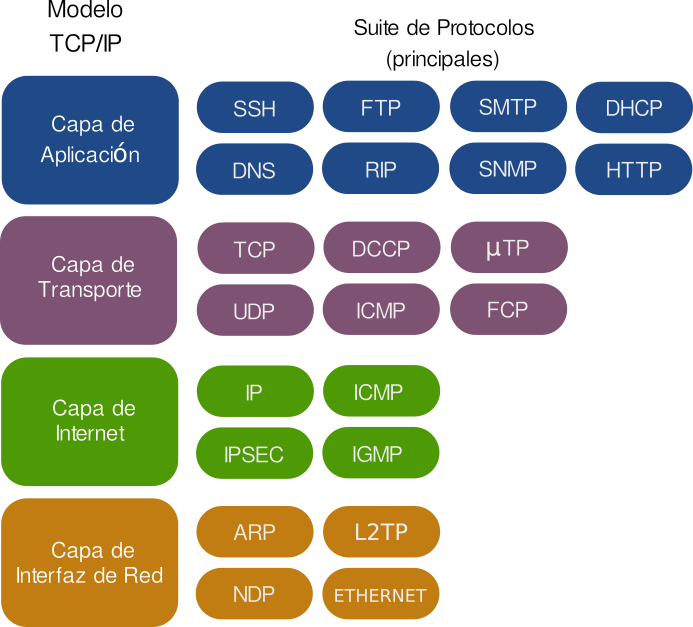
\includegraphics[width=0.8\textwidth]{tcpip}
	\caption{Principales protocolos usados en las cuatro capas de TCP/IP}
	\label{fig:tcpip}
\end{figure}

Existen, independientemente del modelo, diferentes términos que destacan en los ataques a redes, como son el \textit{sniffing}, el \textit{spoofing} o el \textit{hijacking}.

\subsubsection{Sniffing}

El \emph{sniffing} es una técnica que consiste en capturar los paquetes o tramas que pasan por cierta interfaz \cite{ataque-en-redes-ip}. Por defecto un sistema rechaza el tráfico que no está dirigido a él. En cambio, si un sistema actúa en modo promiscuo, aceptará todos los paquetes que le lleguen por la red. El sniffing es la técnica que obtiene todos esos paquetes. Para hacerlo, se hacen uso de herramientas llamadas \textit{sniffers}, que permiten capturar estos paquetes y analizar su información capa por capa.

\subsubsection{Spoofing}

\emph{Spoofing} es un concepto que consiste en suplantar la identidad \cite{ataque-en-redes-ip}. Existen numerosas técnicas de suplantación como por ejemplo \textit{MAC Spoofing}, donde se suplanta la dirección física de un dispositivo. También existen otras como \textit{ARP Spoofing}, \textit{DNS Spoofing} o \textit{Web Spoofing}. Consisten básicamente en falsear cierta información para hacernos pasar por otro usuario, otro nodo u otra aplicación en la red.

\subsubsection{Hijacking}

Se conoce como \emph{hijacking} a toda técnica en la que se obtiene el control de un elemento de una red, de tal manera que se pueda modificar la información que pasa por dicho elemento \cite{ataque-en-redes-ip}. Existen, al igual que con el spoofing, numerosas técnicas que hacen uso del concepto, como por ejemplo \textit{Session Hijacking} o \textit{Browser Hijacking}. De este tipo de técnicas surgen los ataques MITM (\textit{Man In The Middle}), que como su nombre indica, consisten en interferir en la comunicación entre dos nodos para tanto suplantar la identidad del usuario como para recibir información que se supone que solo debería recibirla directamente el usuario.
\chapter{Conclusiones}

A lo largo de los capítulos anteriores se ha realizado un profundo análisis sobre el campo de la seguridad informática, explicando una gran cantidad de conceptos. Primero se han definido una serie de conceptos básicos sobre seguridad informática, intrínsecos a cualquier especialidad o aplicación, como son los servicios de la seguridad de la información.

Por otra parte se ha elaborado un estado del arte de las diferentes aplicaciones de la seguridad informática, comenzando desde el surgimiento de la necesidad de proteger la información y de hacer que las transmisiones de datos fuesen seguras. Se hace un énfasis en el malware y en los tipos que existen, mostrando de que manera somos vulnerables a ataques y en que medida nuestra información esta desprotegida. 

Además, se desmonta el concepto tan arraigado en las mentes de los usuarios de que la seguridad informática consiste en proteger ordenadores personales de malware. Por una parte el malware no es la única amenaza existente, las intrusiones a redes o lo ataques de ingeniería social son otras formas mediante las que se puede acceder a nuestra información. También hay que tener en cuenta que no solo los ordenadores personales son el único target, los avances en diferentes campos, destacando los smartphones, el IoT y el Cloud Cmputing, hace que estos sean actualmente vértices de enfoque importantes dentro de la seguridad informática.

Tras ese análisis sobre el mundo de la seguridad informática, conocer los diferentes sistemas y sus medidas de seguridad, mencionar diferentes tecnologías y enumerar y describir diferentes tipos de vulnerabilidades se puede obtener una idea clara sobre la seguridad informática. Aun así, esta idea no estará completa si no se conoce como actuar ante estas amenazas, como un hacker actúa para conseguir información de un sistema. Por ello se ha hecho especial hincapié en el pentesting. El pentesting es una técnica que mediante la imitación del comportamiento de un atacante permite detectar y explotar vulnerabilidades. Dista de un atacante malicioso, o \textit{Black Hat Hacker}, en que el pentester usa el hacking ético y una serie de procedimientos definidos y controlados con el objetivo de detectar vulnerabilidades de todo tipo para poder posteriormente corregirlas, haciendo los sistemas más seguros. Esta técnica, que requiere un profundo conocimiento de los vectores de ataque y vulnerabilidades, además de sólidas nociones sobre redes y sistemas, permite comprender mejor, ya no solo como defenderse, sino como atacar, dando una visión mas global del conjunto.

\section{La seguridad informática y los usuarios}

Ante esto se plantea un problema serio con respecto a la seguridad de la información. El estado del arte elaborado contiene una gran cantidad de información sobre la seguridad informática, pero no es algo que un neófito en la materia pueda comprender. La seguridad informática es un campo técnico que requiere de una gran cantidad de conocimientos para poder aplicar sus medidas. Por lo tanto, ¿la seguridad de la información de los usuarios solo puede mantenerse mediante el trabajo de los profesionales de la seguridad? ¿Los usuarios no pueden de manera proactiva controlar sus sistemas haciendo que sean estos más seguros?

Aquí es donde entra en juego la programación. ¿Cómo? Elaborando software que pueda usar cualquier usuario, implementando funcionalidad que permita hacer lo que un hacker realiza en su trabajo, pero de una manera clara y sencilla para el usuario, alejado de aspectos técnicos. Esa es la clave para hacer que los usuarios sean un elemento activo en pro de la seguridad de la información.

Pongamos un ejemplo práctico. Si uno se pone en la piel de un pentester, y quiere hacer un ataque de penetración en una red concreta, buscará vulnerabilidades para poder acceder. También puede querer encontrar maneras para defenderse o detectar elementos en una red. El pentester, un hacker con profundos conocimientos del área, sabe que uan de las mejores herramientas de escaneo de redes es NMap\footnote{https://nmap.org/}. Mediante un par de comandos en su terminal obtendrá la información que necesita. De esa manera tan simple podrá proseguir con su trabajo.

Ahora pongamos otro caso. Si, en este caso, uno se pone en la piel de un usuario común que simplemente quiere evitar intrusos en su red local. Algo que seria trivial para un hacker o alguien con conocimientos de redes, resulta bastante complicado para un usuario normal. Dicho usuario no conoce ni NMap ni otras herramientas, no sabe ni siquiera acceder a su router para configurarlo, mucho menos sabe sobre redes o sistemas. Entonces, ¿cómo podría saber si tiene intrusos en su red? ¿La única opción que tendría sería recurrir a alguien con conocimientos sobre el tema?

\section{Herramientas de seguridad informática para usuarios}

En ese tipo de casos es donde entra a colación el software, y como este puede ayudar a los usuarios a llevar a cabo este tipo de tareas. Si queremos ofrecer una solución para el usuario, en base a lo aprendido en puntos anteriores podemos obtener varias conclusiones. Lo primero es que, debido al auge de los smartphones, nuestro software debería programarse para uno de estos sistemas. Si debe ir para uno de estos sistemas, y teniendo que elegir uno, lo mas lógico sería elegir Android, por las cuotas de mercado mencionadas anteriormente. Por otra parte, nuestra aplicación se va a basar en la recogida de información, proceso al que en un pentesting llamábamos \textit{Information Gathering}, por lo que conocer como un pentester recoge la información es fundamental para desarrollar dicha aplicación. Después se puede entrar en que herramientas concretas se puede usar. NMap parece a primera vista la opción mas viable dentro de ese campo. También hay que tener en cuenta herramientas de desarrollo concretas o herramientas secundarias que también pueden ser útiles.

En la siguiente parte de esta memoria se desarrollará una aplicación con lo mencionado en el párrafo anterior (y algunas herramientas más). Se explicaran en detalles las tecnologías y herramientas usadas y todo el proceso de desarrollo de la aplicación, tanto de programación como de diseño de la interfaz o de la experiencia de usuario, con el objetivo de implementar una prueba de concepto que permita vislumbrar cómo llevar herramientas de seguridad informática a usuarios comunes.

\part{Fase 2: Desarrollo de la aplicación}
\chapter{Introducción}

\epigraph{\textit{''La mejor forma de predecir el futuro es implementarlo''}}{--- David Heinemeier Hansson}

{\color{red} Explicar tras el estado del arte en que va a consistir la aplicación.}
\chapter{Tecnologías y herramientas}

\epigraph{\textit{''Java es lo más penoso que le ha ocurrido a la informática desde MS-DOS''}}{--- Alan Kay}

Durante el próximo capítulo se hablará de las herramientas que se usarán para diseñar, desarrollar, documentar y gestionar el desarrollo de la aplicación mencionada. Desde lenguajes de programación, frameworks, SDKs e IDEs hasta herramientas de control de versiones y herramientas secundarias que, si bien no sirven directamente para desarrollar software, sirven como apoyo para otras partes del proceso de desarrollo de la aplicación.

\section{Kali Linux}

Kali Linux\footnote{\url{https://www.kali.org/}} es un sistema operativo basado en Debian que tiene como propósito ofrecer una gran cantidad de herramientas relacionadas con el mundo de la seguridad informática. Es sucesor directo de la conocida distribución BackTrack Linux. Abarca todo tipo de áreas como el \textit{Data Gathering}, \textit{Spoofing} de diferentes tipos, herramientas forenses o ataques a redes inalámbricas, por mencionar solo algunos ejemplos. Es una de las distribuciones más usadas por pentesters y expertos en seguridad informática, en la que se recogen cientos de herramientas concretas, algunas de las cuales son consideradas herramientas de trabajo fundamentales para cualquier hacker, como por ejemplo \textit{Metasploit Framework}, \textit{Johnny The Ripper} o \textit{Nmap}. Esta última será la herramienta que usaremos para dotar a nuestra aplicación de capacidad para obtener información.

Se usará Kali para realizar diversas pruebas con Nmap, previo paso a la integración en la aplicación, para posteriormente poder programar la aplicación que extraerá información de dicha herramienta.

%------------------------------------------------------------------------------

\section{Nmap}

Nmap\footnote{\url{https://nmap.org/}} es un software de escaneo de redes muy usado en auditorías de seguridad. Permite obtener una gran cantidad de información de diferentes nodos o redes, como los servicios que ofrecen, información sobre el sistema operativo o el CMS y sus versiones, qué tipo de filtrado de paquetes realizan, etc.

Nmap es la herramienta de su categoría más usada por varias razones. La primera es que es software libre, con todas las ventajas que eso conlleva: es gratuito, está bien documentado y tiene una comunidad detrás que le da soporte y va mejorándolo y añadiéndole funcionalidades constantemente. Lo segundo es que posee una gran cantidad de herramientas adicionales, teniendo hasta una GUI (\textit{Zenmap}) y un lenguaje propio (\textit{Nmap Scripting Engine, NSE}) que permite crear scripts específicos que Nmap es capaz de ejecutar independientemente del sistema operativo en el que se esté ejecutando.

Se usará Nmap como base para realizar las diferentes operaciones de escaneo de redes. Más adelante se explicará el proceso de integración en la aplicación y cómo se extrae la información que Nmap nos proporciona para usarla en nuestra aplicación.

%------------------------------------------------------------------------------

\section{Android}

Android es un sistema operativo creado en 2005 y que actualmente posee Google. Aun así, el sistema operativo mantiene lo que se denomina el AOSP (\textit{Android Open Source Project}), el cual garantiza que Android siga siendo software libre.

Esto hace que desarrollar para esta plataforma sea completamente gratuito. Si a eso se añade la extensa documentación que existe para desarrollar para esta plataforma, hace que sea una plataforma hacia la cual cada vez más desarrolladores se lanzan a, valga la redundancia, desarrollar aplicaciones en ella.

La elección de este sistema operativo es el paso más lógico teniendo en cuenta que, como se ha mencionado anteriormente, es el sistema operativo con mayor numero de usuarios y además es el que mayores facilidades ofrece para desarrollar.

\subsection{Android SDK}

Se puede desarrollar para Android mediante diversas herramientas, pero la más común de todas es hacer directamente uso del Android SDK (\textit{Software Development Kit}). El SDK nos proporciona todas las herramientas que necesitamos para desarrollar, compilar y depurar aplicaciones para Android.

Existen alternativas que nos abstraen de las capas más bajas de la programación, como puede ser el uso de frameworks multiplataforma que a su vez hacen uso de tecnologías web, como \textit{Phonegap} o \textit{Ionic}. Este tipo de frameworks convierten en triviales una gran cantidad de tareas que requerirían un mayor tiempo de programación, además de que, mediante el uso de tecnologías web como HTML, CSS y JavaScript, permiten un desarrollo multiplataforma y elaborar interfaces gráficas en una menor cantidad de tiempo.

Por otra parte, se podría optar por soluciones para desarrollar en Android a más bajo nivel, como es el Android NDK (\textit{Native Development Kit}), que permite compilar código C++ para Android, con el aumento de rendimiento que eso conlleva al evitar que nuestro código pase por la MV Dalvik, o permitiendo el uso de librerías complejas que tengamos previamente desarrolladas en dicho lenguaje.

No se va a optar por ninguna de las soluciones mencionadas en los dos parrafos anteriores por varios motivos. Por una parte, si bien es cierto que dichos frameworks simplifican, \textit{a priori}, el desarrollo de ciertas aplicaciones, estas aplicaciones suelen encontrarse limitadas en funcionalidad y, para lo que se pretende desarrollar en este proyecto concreto, no servirían debido a la necesidad del uso de librerías externas complejas.

Por otra parte, se evita el uso del NDK ya que, al no tener la necesidad de aplicar cambios en las librerías externas y además dichas librerías, que usaremos compiladas, ya están optimizadas para obtener el mejor rendimiento posible, carece de sentido el uso del NDK, con lo que se simplifica el proceso de desarrollo.

\subsection{Kotlin}

Una vez optado por programar directamente con el SDK de Android y habiendo dejado a un lado opciones como el uso del NDK o diversos frameworks que proveen de abstracciones, el siguiente paso lógico consiste en la elección de un lenguaje de programación para programar la aplicación. La elección de dicho lenguaje obedece a varios factores. En primer lugar, no se puede desarrollar cualquier tipo de aplicación con cualquier lenguaje. Por ejemplo, a nadie se le ocurriría usar C++ para desarrollar el frontend de una aplicación web, de la misma manera que pocos se atreverían a usar Lisp para el desarrollo de videojuegos. Por otro lado, las características específicas de un lenguaje u otro son determinantes a la hora de elegir entre ellos. A eso se le añade que resulta mala práctica usar un criterio personal a la hora de elegir un lenguaje especifico.

Teniendo eso en cuenta, la primera opción para desarrollar aplicaciones con el SDK de Android sería Java, ya que es el lenguaje en el que está programado dicho kit. Por otra parte Java es un lenguaje con un largo recorrido y actualmente, según el índice TIOBE, es el lenguaje de programación más usado \cite{tiobe}, ocupando el primer puesto en su ranking. Tiene una gran comunidad a su alrededor y gran parte de el software que usamos actualmente está desarrollado con él.

Sin embargo, se ha optado por elegir Kotlin como lenguaje de programación. Kotlin\footnote{\url{https://kotlinlang.org/}} es un lenguaje de programación, (publicado bajo la licencia Apache) que se ejecuta en la JVM y cuyo desarrollo comenzó y es supervisado por JetBrains, compañia que dasarrolla IDEs y plugins para desarrollar aplicaciones. Tiene como principal objetivo convertirse en un sustituto viable de Java, corrigiendo los defectos que este último tiene y aportando nuevos elementos a su sintaxis que permitan facilitar el desarrollo y obtener un código más limpio y claro.

Se ha optado por el uso de Kotlin por varios motivos. El primero es que aporta numerosas ventajas con respecto a Java que, como se ha mencionado, permiten elaborar un código más limpio y fácil de entender. Por otra parte es completamente interoperable con Java, por lo que se complementa a la perfección con partes de código escritas en Java. A todo esto se le añade que recientemente Android ha adoptado a Kotlin como lenguaje oficial \cite{kotlin-android}, por lo que su uso no dará problemas en Android. Eso además hará que se encuentre documentación oficial sobre el uso de Kotlin en dicho sistema, lo que simplificará el desarrollo de la aplicación.

\subsubsection{Ventajas de Kotlin}

A nivel de programación Kotlin representa una mejora notable con respecto a Java, tanto a nivel de código, añadiendo nueva sintaxis, como la funcionalidad adicional que aporta la librería estándar del propio lenguaje. Aunque la lista de mejoras, añadidos y aspectos que se han decidido eliminar con respecto a Java es excesivamente larga como para mostrarla completamente, a continuación se enseñan algunos aspectos del lenguaje que permiten vislumbrar las ventajas que ofrece frente a Java \cite{kotlin-vs-java}.

\paragraph{Control de referencias nulas}

Kotlin corrige uno de los principales problemas del desarrollo de aplicaciones en Java, que son los \textit{Null Pointer Exceptions}. Kotlin es mucho más seguro a ese nivel ya que, por defecto en Kotlin, una variable no puede ser nula, y si queremos que esa variable tenga la posibilidad de ser nula debemos usar un operador específico (el operador \mintinline{java}{?.}).

\begin{minted}[
tabsize=4,
frame=single,
framesep=2mm,
baselinestretch=1.2,
fontsize=\footnotesize,
linenos,
breaklines
]{java}

var a: String = "abc"
a = null // Error de compilacion

var b: String? = "abc"
b = null // Ok

\end{minted}

De la misma manera, se puede especificar en la declaración de una función si esta puede devolver o no un valor nulo. Kotlin no permite asignar un valor que independientemente del tipo que sea, pueda ser nulo a una variable que no pueda serlo.

\begin{minted}[
tabsize=4,
frame=single,
framesep=2mm,
baselinestretch=1.2,
fontsize=\footnotesize,
linenos,
breaklines
]{java}

fun foo(node: Node): String? {
	if(node.canString()) {
		return node.toString()
	}
	else {
		return null // Esto funciona
	}
}

fun foo2(node: Node): String {
	return null // Error de compilacion
}

\end{minted}

De ahí que, si queremos usar una función que pueda devolver un valor nulo o obtener un atributo de una instancia que pueda ser nulo tendremos tres opciones:

\begin{enumerate}
	\item Comprobar si es nulo antes de usar el operador: Kotlin detecta automáticamente si se ha realizado una comprobación de este tipo, y una vez hecha nos permitirá realizar este tipo de operaciones.
	
\begin{minted}[
tabsize=4,
frame=single,
framesep=2mm,
baselinestretch=1.2,
fontsize=\footnotesize,
linenos,
breaklines
]{java}

var b: String? = "abc"
if (var != null) {
	var c: String = b // Esto si se permite, ya que ahora sabemos que no es null
}
var d: String = b // Esto da error, puede ser null

\end{minted}

	\item Usar el operador seguro \mintinline{java}{?.}: en este caso, si el valor existe o la función no devuelve un valor nulo todo funcionará correctamente, si no devolverá un valor nulo.
	
\begin{minted}[
tabsize=4,
frame=single,
framesep=2mm,
baselinestretch=1.2,
fontsize=\footnotesize,
linenos,
breaklines
]{java}

var b: String? = "abc"
var len: Int? = b?.length // Si b no es null devuelve la longitud (3)
var len2: Int = b?.length // Esto da error, puede ser null

\end{minted}

	\item Usar el operador \mintinline{java}{!!.}: Este operador es mucho más peligroso. En caso de tratar con valores nulos genera directamente una \textit{Null Pointer Exception}. La ventaja es que permite que las variable sean siempre no nulas.
	
\begin{minted}[
tabsize=4,
frame=single,
framesep=2mm,
baselinestretch=1.2,
fontsize=\footnotesize,
linenos,
breaklines
]{java}

var b: String? = "abc"
var len: Int? = b!!.length // Si b no es null devuelve la longitud, si no salta un NPE
var len2: Int = b!!.length // Esto NO da error, porque en caso de ser null saltará un NPE

\end{minted}

\end{enumerate}

\paragraph{Atributos de una clase}

Kotlin dispone de mecanismos para generar automáticamente funciones \textit{getter} y \textit{setter}, de tal manera que se ahorra ese engorroso código que se genera en muchas clases de aplicaciones programadas en Java. Por otra parte se puede modificar estas funciones de manera muy sencilla para que cumplan diversos objetivos, usando menos código que en Java.

\begin{minted}[
tabsize=4,
frame=single,
framesep=2mm,
baselinestretch=1.2,
fontsize=\footnotesize,
linenos,
breaklines
]{java}

class Lista {

	// ...
	
	var elementos
		get() {
			return elementos.filterNotNull()
		}
		set(value) {
			if(value != null)
				elementos.add(value)
		}
	val isEmpty: Boolean
		get() = elementos.size == 0
	
	// ...

}
\end{minted}

\paragraph{Singletons}
Se puede hacer uso del patrón Singleton usando la palabra \mintinline{java}{object} en vez de \mintinline{java}{class} a la hora de crear la clase en cuestión, de tal manera que Kotlin se encarga de que solo haya una instancia de esa clase.

\begin{minted}[
tabsize=4,
frame=single,
framesep=2mm,
baselinestretch=1.2,
fontsize=\footnotesize,
linenos,
breaklines
]{java}

class PDF {
	// ...
}

object PDFManager {
	// ...
}

var pdf1 = PDF() // Ok
PDFManager.AddPDF(pdf1) // Se accede a sus funciones y variables como si fuera una variable normal
var manager = PDFManager() // Error de compilacion. No se pueden crear instancias de un singleton, porque Kotlin ya crea la unica instancia posible

\end{minted}

\paragraph{Data Classes}

Kotlin tiene un tipo de clases especial para cuando se desea una clase que solo almacene información y carezca de funcionalidad, denominado Data Classes, que permite ciertas ventajas a la hora de realizar comparaciones o copiar datos, y reduce sensiblemente la cantidad de código de la clase.

\begin{minted}[
tabsize=4,
frame=single,
framesep=2mm,
baselinestretch=1.2,
fontsize=\footnotesize,
linenos,
breaklines
]{java}

data class User(val name: String, val age: Int)
data class User(val name: String = "", val age: Int = 0)

\end{minted}

\paragraph{Expresiones de rango}

Kotlin, al igual que otros lenguajes como Python, permite expresiones de rango, que nos permiten iterar sobre rangos de numeros de forma muy sencilla: además permite determinar la cantidad de aumento o disminución en cada iteración, como se puede observar en los siguientes ejemplos.

\begin{minted}[
tabsize=4,
frame=single,
framesep=2mm,
baselinestretch=1.2,
fontsize=\footnotesize,
linenos,
breaklines
]{java}

for (i in 1..4 step 2) 
	print(i) // imprime "13"
for (i in 4 downTo 1 step 2)
	print(i) // imprime "42"

\end{minted}

Aunque existen aun más, con las ventajas mostradas anteriormente queda claramente reflejada la ventaja de programar aplicaciones en Kotlin con respecto a hacerlo en Java.

\subsection{Android Studio}

Android Studio es un IDE que posibilita desarrollar para Android de manera mucho más cómoda. Permite hacer uso del SDK y, asimismo, nos provee de una serie de herramientas, como herramientas de diseño de interfaces gráficas, herramientas de depuración o dispositivos Android virtuales, además de otras ventajas que suele conllevar el uso de un IDE como el autocompletado de código, la automatización de la compilación y el desarrollo o herramientas de análisis de rendimiento. Se trata de un fork del conocido IDE \textit{IntelliJ IDEA}, de la compañia JetBrains, al que se le han añadido las herramienteas necesarias para programar en Android.

Es el IDE que se usará para desarrollar la aplicación porque, por una parte, es el que recomienda Android ya que está especialmente diseñado con el propósito de desarrollar aplicaciones para su plataforma y, por otra parte, tiene soporte para Kotlin.

%------------------------------------------------------------------------------

\section{Otras herramientas}

Una vez mencionadas herramientas que permiten desarrollar la aplicación se pasa a mencionar herramientas que, aunque no influyen directamente en la programación de la aplicación, merecen especial mención porque influyen de manera indirecta y se usan para el desarrollo del proyecto.

\subsection{Git}

Git\footnote{\url{https://git-scm.com/}} es un Sistema de Control de Versiones o VCS (\textit{Version Control Systems}) distribuido y de código libre desarrollado por Linus Torvalds en 2005 con el objetivo de llevar un control sobre el desarrollo del Kernel Linux. Es a día de hoy uno de los VCS más usados, tiene diferentes implementaciones para una gran cantidad de sistemas y dispone de una amplia documentación. 

El uso de este VCS tiene como objetivo poder llevar un control sobre el desarrollo y el avance de nuestro código, pudiendo revertir cambios, crear diferentes ramas en el desarrollo para desarrollar diferentes funcionalidades por separado o actuar como sistema de backup mediante el uso de un repositorio remoto que puede esta alojado en servicios de alojamiento de repositorios como GitHub\footnote{\url{https://github.com/}} o similares.

\subsection{\LaTeX}

LaTeX\footnote{\url{http://www.latex-project.org/}}  es un sistema de composición de textos que permite crear todo tipo de documentos. Suele ser utilizado para escribir de artículos académicos, tesis y libros técnicos debido a que los documentos generados con él son de alta calidad, llegando al nivel de una editorial profesional, con la ventaja de que es completamente libre.

Se usará LaTeX, junto una serie de librerías específicas, para el desarrollo de este informe por la calidad de los documentos que genera y por ser prácticamente un estándar dentro de la comunidad científica y académica. 
\chapter{Desarrollo de la aplicación}

\epigraph{\textit{''Los programas deben ser escritos para que los lean las personas, y sólo incidentalmente, para que lo ejecuten las máquinas''}}{--- Abelson and Sussman}

\begin{comment}
Tras haber explicado en el capítulo anterior las diversas herramientas a usar para el desarrollo de la aplicación, en este capítulo se explicaran aspectos sobre el diseño de la aplicación y las diferentes decisiones tomadas a la hora de realizar dicho diseño.

El diseño de la aplicación es simple minimista. El objetivo del proyecto consiste en hacer una aplicación lo mas fácil de usar y con la mayor claridad posible de cara al usuario. Por ello, se ha optado por un enfoque que reduzca el numero de elementos al mínimo, ademas de que se adapta perfectamente a los estándares de diseño de Materia Design, que son los recomendados a la hora de diseñar aplicaciones para Android.

\section{Interfaz gráfica}

Para la interfaz gráfica se ha optado por hacer un diseño primero en papel para después, en base a ese diseño y esa distribución de ventanas, elaborar en Android Studio toda la interfaz gráfica. Se puede observar un diseño primitivo en la siguiente imagen.

\begin{figure}[H] % TODO: REPLACE THIS PLACEHOLDER WITH THE TRUE IMAGE
	\centering
	
\includegraphics[width=200px]{placeholder}
	\caption{Mockup inicial de la GUI de la aplicación}
	\label{fig:mockup}
\end{figure}

La aplicación esta dividida en varias vistas. Debido a que el objetivo principal de la aplicación es que sea lo mas simple posible, se ha diseñado buscando minimizar el numero de ventanas de la aplicación.

A la hora de crear las vistas en Android se usan dos conceptos. \textit{Activity} y \textit{Fragment}. En Android, una Activity representa una parte de la UI de una aplicación, y tiene su propio ciclo de vida y su propia jerarquía de elementos. Una aplicación Android dispone de tantas Activity como el usuario quiera implementar, entendiendo que cada Activity servirá para mostrar cierta información e interactúa con el usuario de una manera concreta. A continuación se muestra el ciclo de vida de una Activity, con los métodos que se ejecutan en ciertos puntos

\begin{figure}[H]
	\centering
	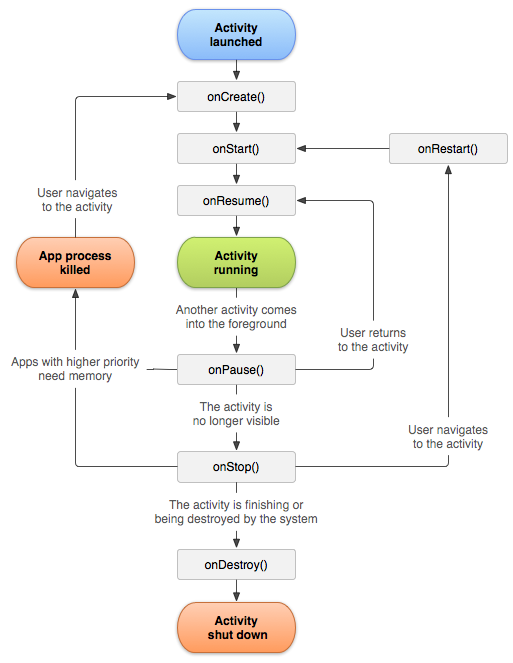
\includegraphics[width=0.75\textwidth]{activity-lc}
	\caption{Ciclo de vida de una Activity de Android}
	\label{fig:activity-lc}
\end{figure}

El Fragment, aunque también representa una parte de la UI de la aplicación, depende de una Activity, ya que debe acoplarse a una. A diferencia del Activity, se pueden mostrar varios Fragments a la vez. Hay que tener en cuenta que un Fragment, aun teniendo su propio ciclo de vida (más simplificado que el del Activity) depende del ciclo de vida del Activity al que este acoplado. 

\begin{figure}[H]
	\centering
	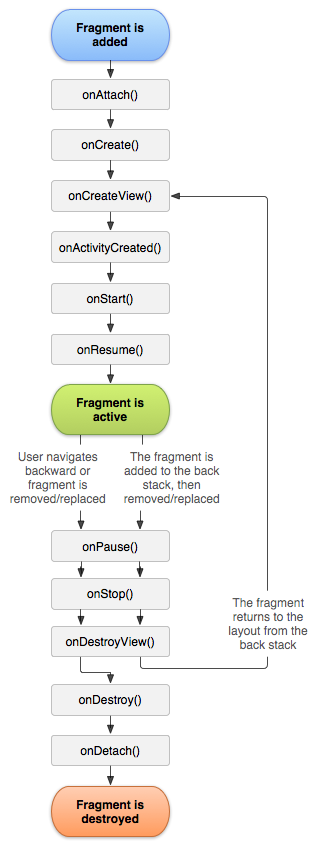
\includegraphics[height=0.75\textheight]{fragment-lc}
	\caption{Ciclo de vida de un Fragment de Android}
	\label{fig:fragment-lc}
\end{figure}


En Android, a la hora de diseñar aplicaciones, se usan fragments para partes reutilizables y comunes de una UI y se usan las activitys para controlar el ciclo de vida de la aplicacion. En uan aplicación de android abierta siempre se encuentra activa una activity, que muestra algun tipo de interfaz.

La apicacion dispone de la siguiente lista de activitys y fragments
\end{comment}
\chapter{Implementación de la aplicación}

\epigraph{\textit{''Talk is cheap. Show me the code''}}{--- Linus Torvalds}

Dentro del desarrollo de la aplicación, la parte que se puede considerar como la más importante es la parte de la implementación. Tomando en base todo el diseño, tanto a nivel conceptual, gráfico o de software, se ha implementado la aplicación, siendo esta uno de los dos objetivos del proyecto.

En este capítulo se explican los diferentes aspectos del proceso de desarrollo, tanto como se ha implementado la persistencia de datos, los escaneos que realiza la aplicación y todo tipo de consideraciones que se han tenido en cuenta durante la implementación y que merece la pena mencionar.

Este capítulo no pretende ser ni una descripción de cada elemento que forma parte del código, ni una documentación formal como puede ser la documentación de una API. Por razones de espacio y claridad, no se incluye todo el código desarrollado, tanto porque entorpecería las explicaciones de como se ha ido desarrollando y como se ha ido implementado la aplicación como porque haría este informe del proyecto excesivamente grande.

\section{Estructura del proyecto}
El código del proyecto se puede dividir en dos grandes bloques. Por una parte disponemos de los ficheros que contienen código en Kotlin y por otra parte los ficheros XML que definen, tanto layouts, elementos que se pueden dibujar o variables asociadas a las diferentes cadenas de caracteres (de ahora en adelante \textit{strings}) o a variables numéricas como colores o dimensiones.

El propio entorno de Android Studio permite diferencias ambos tipos de archivos, disponiendo del código en la carpeta \textit{java} (el nombre puede llevar a confusión, pero es el nombre por defecto en la creación de proyecto, aunque contenga únicamente código en Kotlin) y de los diferentes archivos XML en la carpeta \textit{res}. Esta última a su vez se divide en diferentes carpetas para organizar los archivos XML en función de su utilidad.

\begin{figure}[H]
	\centering
	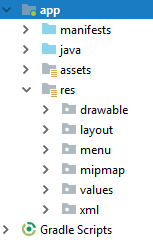
\includegraphics{basic-android-studio-structure}
	\caption{Estructura básica de archivos del proyecto}
	\label{fig:basic-android-studio-structure}
\end{figure}

Otras carpetas importantes son las carpetas de \textit{manifests} y la carpeta de \textit{assets}. En la primera es donde se guardan los diferentes \textit{Manifest} de la aplicación. Un Manifest\footnote{\url{https://developer.android.com/guide/topics/manifest/manifest-intro}} en Android es un fichero XML donde se definen una serie de variables importantes a nivel global con respecto a la aplicación. Entre otras funciones, es donde se define el nombre de la aplicación, su icono y sus diferentes componentes, que pueden ser Activities, Services, BroadcastReceivers o ContentProviders.

Por otra parte mencionar la existencia de diferentes scripts de Gradle, que es el sistema de automatización de construcción de aplicaciones más usado en Android para compilar el código y generar la aplicación ejecutable, entre otras cosas.

\subsection{Estructura de paquetes de código}

Dentro de la carpeta \textit{java}, debido a la gran cantidad de ficheros de código Kotlin, existe una estructura de paquetes que divide los ficheros de código en diferentes categorías. Cada uno de los ficheros de código existentes implementa una única clase, interfaz o tipo enumerado. Esto es así para mantener cada elemento claramente visible y al mismo nivel y a su vez evitar archivos excesivamente grandes que compliquen entender el código. La estructura de paquetes se muestra en la Figura \ref{fig:android-studio-package-structure}.

\begin{figure}[H]
	\centering
	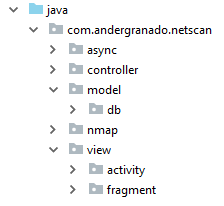
\includegraphics{android-studio-package-structure}
	\caption{Estructura de paquetes de código del proyecto}
	\label{fig:android-studio-package-structure}
\end{figure}

En los paquetes \textit{model}, \textit{controller} y \textit{view} se implementan las diferentes partes de las que está formada una aplicación que sigue el patrón MVC (Model View Controller). Es un patrón largamente usado a la hora de diseñar aplicaciones con interfaz gráfica, que consiste básicamente en dividir los datos (Model), las diferentes vistas de la aplicación (View) y la parte que actúa como puente entre los datos y las vistas (Controller) en entidades separadas. Esto permite que el codigo generado sea escalable, legible y elimine dependencias innecesarias. 

En el caso de Android, las diferentes vistas se implementan en diversas Acitivities y Fragments. El modelo es básicamente una serie de clases (algunas de ellas Data Classes de Kotlin) que definen los diferentes datos que existen, tanto para la aplicación como datos concretos que son persistentes en la aplicación (separados en el paquete \textit{db}) y los controladores están implementados usando RecyclerViews de Android, cuyo funcionamiento se explicará más adelante.

Por último, mencionar los paquetes \textit{async} y \textit{nmap}. El paquete \textit{async} contiene toda aquella funcionalidad que se ejecuta de manera paralela o asíncrona, como diferentes AsyncTasks o clases que se basan en la ejecución de Threads o hilos. El paquete \textit{nmap} contiene todo el código necesario para implementar Nmap en la aplicación, tanto para instalarlo, ejecutarlo como para interpretar los datos que genera. Todo el código que hace uso de Nmap se encuentra en este paquete, dejando el resto de la aplicación completamente aislada de las particularidades de Nmap

\section{Integración de Nmap}

Integrar soluciones de terceros en una aplicación o un sistema que está en desarrollo puede ser desde algo simple, más bien mecánico, a todo un quebradero de cabeza, en función del tipo de software o funcionalidad que queramos añadir desde fuera.

En concreto, a la hora de integrar Nmap en la aplicación hay que tener en cuenta una serie de factores. Integrar Nmap en una aplicación difiere completamente de integrar, por ejemplo, una librería con una API definida. Integrar una librería en una aplicación consiste simplemente en una serie de pasos para configurar esa librería que, una vez realizados, nos permiten mediante una interactuar mediante una API con esa librería y aprovechar toda la funcionalidad que nos provee. 

En cambio, con Nmap es radicalmente diferente. Debido a que Nmap no es una librería, sino un software complejo que nos permite analizar redes de ordenadores, no podemos integrarlo como si de una librería se tratase. Por lo tanto, debemos buscar otros métodos diferentes para integrarlo.

Nmap es una solución de código libre que lleva siendo desarrollada por la comunidad que ha generado alrededor durante más de 10 años. Cabría pensar que una posibilidad para integrar la funcionalidad de Nmap en la aplicación es obtener su código fuente (que al ser software libre es público y está disponible para su uso) e integrarlo directamente en el proyecto.

El principal problema de esta posibilidad es que Nmap es un software muy complejo. El núcleo de Nmap está desarrollado en C, pero también diversas partes están desarrolladas en lenguaje es como Lua, C++ o Python, como se puede observar en la FIGURA de su repositorio\footnote{\url{https://github.com/nmap/nmap}}. Esto impide que podamos introducir todo ese código en lenguajes no soportados por Android en el proyecto, haciendo que Nmap no se pueda integrar directamente a nivel de código.

\begin{figure}[H]
	\centering
	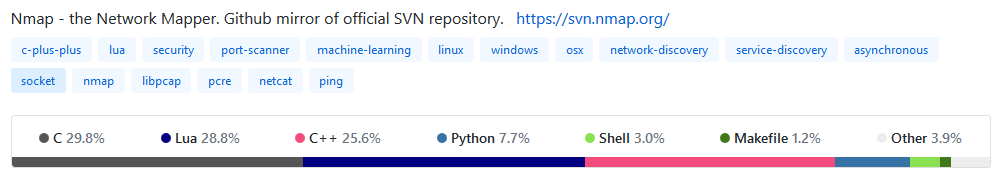
\includegraphics[width=1.0\textwidth]{nmap-repo-languages}
	\caption{Distribución de lenguajes en el repositorio de Nmap}
	\label{fig:nmap-repo-languages}
\end{figure}

Es cierto que se puede, mediante el uso del NDK de Android, introducir código tanto en C como en C++ en nuestra aplicación. Pero el funcionamiento de Nmap es tan complejo que intentar integrar solamente esa parte del código y esperar que funcione eliminando el resto de módulos sería una tarea tan titánica como inútil.

Por ello la última opción, y la única realmente viable, para integrar Nmap en nuestra aplicación es interactuar directamente con archivos binarios de Nmap. Es decir, incluir la aplicación compilada dentro del proyecto, ejecutarla mediante código y obtener e interpretar la información que devuelva.

\subsection{Instalación}

Esto a la vez genera una serie de cuestiones. Si queremos introducir un binario dentro de nuestra aplicación y controlar su ejecución en un dispositivo lo primero que tenemos que tener en cuenta es que la arquitectura para la que ha sido compilada el binario coincida con la arquitectura del dispositivo.

Nmap  es una aplicación que se puede ejecutar tanto en sistemas Windows y OS X como en sistemas basados en Linux. Aunque android es un sistema Linux, Android no se suele ejecutar en las plataformas en las que se suele ejecutar normalmente Linux, que son x86 y x64, arquitecturas Intel. La mayor parte de dispositivos Android son dispositivos con procesadores ARM BUSCAR REFERENCIA,por lo tanto no podemos  ejecutar una versión estándar de Nma para Linux.

Para solucionar esto se puede optar por dos opciones. La primera sería compilar Nmap para arquitecturas especialmente para Android en ARM. Compilar un proyecto de la envergadura de Nmap es una tarea engorrosa y difícil de realizar. La segunda sería buscar binarios ya compilados especialmente para Android. Por suerte existen binarios de Nmap para dispositivos Android.

La propia web de Nmap\footnote{\url{https://secwiki.org/w/Nmap/Android}} nos ofrece binarios de Nmap específicos para Android, la desventaja es que no se trata de binarios oficiales, aunque avalados por Nmap, sino de binarios generados por un usuario concreto\footnote{\url{https://github.com/kost/nmap-android}}. Otra desventaja de estos binarios es que no están completamente actualizados. La versión más reciente de los binarios de Nmap para Android es la 7.31 (25 de octubre de 2016), unas versiones más atrasada desde la última, la 7.70\footnote{\url{http://seclists.org/nmap-announce/2018/0}} (20 de marzo de 2018) que a día de hoy es la última versión de Nmap.

Aunque la última versión disponible de Nmap para Android no está tan actualizada como la última versión de Nmap, hay que tener en cuenta que Nmap es un software con un desarrollo avanzado y que, aunque vaya añadiendo funcionalidad, lleva durante años siendo un software robusto y estable. Por esto utilizar Nmap para Android no debería ser un gran problema.

Nmap para Android viene compilado o para una serie de arquitecturas concretas, como se puede observar en la FIGURA. Aunque tenemos un rango amplio de arquitecturas para elegir, debemos tener en cuenta que nuestro público objetivo es un público general. La mayor parte de móviles Android utilizan procesadores ARM. Aun así, y para garantizar la compatibilidad con todos los dispositivos, se han integrado binarios de Nmap para Android para arquitecturas ARM. x86 y MIPS, con sus equivalentes de 64 bits. Con esto cubriremos todos los dispositivos móviles posibles.

\begin{figure}[H]
	\centering
	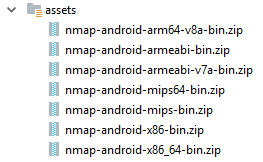
\includegraphics{project-assets}
	\caption{Los diferentes binarios para cada arquitectura usados en la aplicación}
	\label{fig:project-assets}
\end{figure}

La forma de introducir estos binarios en el dispositivo es sencilla y está completamente automatizada. por una parte se almacena cada uno de los diferentes binarios en diferentes ficheros comprimidos en formato ZIP. Cada uno de estos ficheros ZIP se encuentra metido en la carpeta \textit{assets} del proyecto, como se muestra en la Figura \ref{fig:project-assets}. Esta carpeta sirve para guardar todo tipo de recursos que queramos cargar en nuestra aplicación. Recursos como pueden ser ser archivos de texto, imágenes, archivos de audio, y un largo etcétera. Aunque en principio no esté diseñada para guardar binarios y programas completos, en nuestro caso servirá para guardar los ficheros de Nmap y después poder desplegarlos en el dispositivo.

Desplegarlos en el dispositivo es relativamente sencillo. Para ello solo debemos tener en cuenta la arquitectura el dispositivo en el que se está ejecutando la aplicación y descomprimir el archivo con los binarios correspondientes.

La localización donde guardemos los binarios de Nmap es fundamental, ya que según donde se guarden tendremos permiso para ejecutarlos o no. En este caso se guardan en lo que denominamos Internal Storage\footnote{\url{https://developer.android.com/training/data-storage/files}} de Android. Dentro de la estructura de archivos de Android existe una carpeta llamada \textit{data}, que a su vez tiene otra carpeta del mismo nombre. Dentro de esa última carpeta existe una carpeta por cada aplicación instalada en el sistema. Cada una contiene una aplicación y sus archivos asociados. Esta carpeta sólo es accesible para la propia aplicación, que tiene permisos de lectura, escritura y ejecución dentro de ella, lo que la convierte en el lugar idóneo para depositar los binarios.

Toda este volcado de binarios de Nmap para el dispositivo se gestiona desde una única clase en la aplicación llamada \mintinline{java}{NmapInstaller}. Esa clase, que implementa el patrón Singleton mediante el uso de la palabra clave \mintinline{java}{object} de Kotlin, contiene todo el código necesario para volcar los binarios de Nmap en el dispositivo.

\begin{listing}[H]
	\custominputminted{kotlin}{code/install.kt}
	\caption{Función que instala Nmap en el dispositivo}

	\label{code:install}
\end{listing}

Como se puede observar en el código, dentro de la función \mintinline{java}{install()} se realiza ese volcado pudiendo tener opciones para reescribir los archivos en caso de que se quiere escribir. Estos archivos se cargan a través del Asset Manager y mediante las clases de Java para interactuar con ficheros comprimidos se extraen en los ficheros internos de la aplicación.

A su vez también se actualiza la base de datos de script NSE de Nmap, en caso de que se quiera después ejecutar alguno de esos script. 

\subsection{Ejecución}

Una vez tenemos disponibles todos los binarios de Nmap y archivos necesarios para ejecutar Nmap introducidos e instalados en el dispositivo, el siguiente paso necesario es implementar la funcionalidad que nos permita ejecutarlos.

Todo el código que permite ejecutar en el mapa se encuentra en otra clase llamada \mintinline{java}{NmapRunner}. Esta clase tiene diversos métodos que nos permiten interactuar con los binarios y en última instancia ejecutar escaneos.

Lo que tenemos que hacer para ejecutar un escaneo es ejecutar el binario de Nmap con los parámetros correspondientes. Para ejecutar en el mar basta simplemente con lanzar un proceso que llame a la ejecución del binario. La forma de ejecutar un binario es muy sencilla, y consiste en crear un proceso para una shell de Linux y en el llamar al ejecutable de Nmap. Para poder interactuar con ese proceso necesitamos configurar la entrada y la salida de ese proceso para poder enviarle información y recibirla. Eso se realizan la función \mintinline{java}{startProcess()}, que se muestra a continuación.

\begin{listing}[H]
	\custominputminted{kotlin}{code/startProcess.kt}
	\caption{Función para arrancar el proceso con la shell que ejecutará Nmap}
	
	\label{code:startProcess}
\end{listing}

Después de esto debemos construir un comando de Nmap. Este comando es básicamente lo que haríamos si estuviéramos ejecutando Nmap en la terminal de nuestro ordenador. En nuestro caso solo queremos realizar una serie de escaneos concretos a nodos puntuales, por lo tanto construir este comando es tan sencillo como concatenar unos pocos strings. La función que realiza esto se muestra a continuación.

\begin{listing}[H]
	\custominputminted{kotlin}{code/commandBuilder.kt}
	\caption{Función que crea el comando a ejecutar de Nmap}
	
	\label{code:commandBuilder}
\end{listing}

Una vez realizado esto queda pasar ese comando al proceso y ejecutar Nmap. A partir de aquí podríamos obtener la información del escaneo de dos maneras. La primera sería leer la salida que nos da el proceso en texto plano y extraer la información de. La segunda, mejor alternativa, consiste en ejecutar Nmap de tal manera que la información del escaneo se guarde en un fichero XML.

Las ventajas de utilizar un fichero XML para cobrar esa información son obvias. En un fichero XML dispondremos de la información estructurada que podremos leer utilizando la librería para trabajar con archivos XML que provee el SDK de Android. Por lo tanto, y como se ha podido observar, se añade el parámetro \mintinline{java}{-oX} cuándo se crea el comando a ejecutar, qué es el que indica que la salida se almacene en un fichero XML.

Una vez realizado el escaneo y habiéndose generado ese fichero XML, solo queda obtener la información de ese fichero y deshacernos de todos los recursos ya innecesarios, como el propio fichero XML una vez leído, o el propio proceso de la shell, que consume recursos no necesarios.

\begin{listing}[H]
	\custominputminted{kotlin}{code/runScan.kt}
	\caption{Función con todo el proceso de ejecución de un escaneo en Nmap}
	
	\label{code:runScan}
\end{listing}

\subsection{Leer datos}

La tercera y última parte del proceso para integrar Nmap es leer los datos que han sido generados. Como se ha mencionado dichos datos se encuentran en un fichero XML. Por lo tanto, necesitaremos una clase qué obtenga la informacion de dicho fichero. A este tipo de clases se le suele denominar \textit{parser} y básicamente van leyendo las diferentes etiquetas de los ficheros XML y obteniendo su información. A continuación se muestra ciertas partes del código para hacerse la idea de cómo es leer de manera jerarquizada y estructura de un fichero XML. No se muestra toda la implementación, ya que el tamaño de la implementación de un parser de XML es directamente proporcional al tamaño de la jerarquía de los elementos que contiene.

\begin{listing}[H]
	\customtinyinputminted{kotlin}{code/nmapParser.kt}
	\caption{Extracto de la implementación de un parser de un XML de Nmap}
	
	\label{code:nmapParser}
\end{listing}

Almacenar la información en XML la almacena jerarquizada en cierta manera la manera en la que Nmap guarda información estructurada en un fichero XML es como la que se muestra en el Código \ref{code:regular-scan}:

\begin{listing}[H]
	\customtinyinputminted{xml}{code/regular-scan.xml}
	\caption{Fichero XML con la información de un escaneo estándar de Nmap}
	
	\label{code:regular-scan}
\end{listing}

Sin entrar en detalles sobre el funcionamiento cada una etiqueta se puede observar que se genera una etiqueta \textit{host} por cada uno de los nodos encontrados en el escaneo. Un solo escaneo puede servir tanto para único host como para un rango completo de redes CIDR, por lo que habrá tantas etiquetas host como nodos se hayan detectado.

Dentro de la información generada para cada host, aunque depende del tipo de escaneo realizado, se pueden observar etiquetas que aparecerán para la gran mayoría de casos. Por ejemplo \textit{status}, que nos indica el estado del host, \textit{address}, que nos indica la dirección IP del host, \textit{hostname},que es el nombre que recibe dicho host, o la etiqueta \textit{ports}, qué contiene una lista de todos los puertos abiertos o filtrados que se han encontrado para cada nodo, con información sobre configuraciones, métodos usados para escanearlos o nombres de dichos puertos.

Por último una vez leído ese fichero a medida que se va leyendo ese fichero se va guardando la información en diferentes clases, creadas específicamente para guardar los datos obtenidos de Nmap antes de ser procesados. Dichas clases se encuentran dentro del paquete \textit{model}. En concreto, todas las clases que se usan para datos obtenidos directamente de Nmap llevan el prefijo \mintinline{java}{Nmap}, para diferenciarlas de clases del modelo relacionadas con la estructura de la información en la base de datos. En los Códigos \ref{code:nmapScan}, \ref{code:nmapHost} y \ref{code:nmapPort} se muestran unos ejemplos.

\begin{listing}[H]
	\custominputminted{kotlin}{code/nmapScan.kt}
	\caption{Data Classes para la información de un scan en Nmap}
	
	\label{code:nmapScan}
\end{listing}

\begin{listing}[H]
	\custominputminted{kotlin}{code/nmapHost.kt}
	\caption{Data Classes para la información de un host en Nmap}
	
	\label{code:nmapHost}
\end{listing}

\begin{listing}[H]
	\custominputminted{kotlin}{code/nmapPort.kt}
	\caption{Data Classes para la información de un puerto en Nmap}
	
	\label{code:nmapPort}
\end{listing}

\section{Persistencia de datos}

A día de hoy prácticamente cualquier aplicación, independientemente de si es una aplicación móvil o una aplicación para cualquier otro sistema, requiere almacenar datos de manera persistente. Ya sea desde simples valores para guardar configuraciones o ajustes de usuario a todo un conjunto de datos que se genera, gestiona y define el funcionamiento de dicha aplicación.

En el caso de nuestra aplicación, que tiene cuyo objetivo principal analizar redes informáticas y obtener información, necesitaremos guardar la información de cada uno de esos análisis para que el usuario la tenga siempre accesible en todo momento.

La persistencia de datos una aplicación se puede implementar de diversas maneras, y la elección de una manera u otra obedece a varios factores. Hay que tener en cuenta, entre otras cosas, el volumen de datos que se vaya a generar, la frecuencia con la que se van a modificar esos datos o si esos datos van a ser transferidos en algún momento.

A grosso modo se pueden dividir las formas de implementar persistencia de datos en dos principales tipos: el uso de ficheros o el uso de bases de datos.

El uso de ficheros es el modo más simple de almacenar datos. Consiste en guardar los datos escribiendo en ficheros y en obtener datos leyendo de ellos. Esos ficheros pueden contener los datos en sí mismos o junto a algún tipo de estructura, siendo esta la más sencilla de mantener. Como ejemplos de datos estructurados tenemos una serie de formatos como XML, CSV o JSON.

Por otra parte, tenemos el uso de bases de datos. A medida que los datos crecen en complejidad y en número, se vuelve cada vez más complicado el acceso lectura y escritura dichos datos. El uso de bases de datos permite almacenar una gran cantidad de datos relacionados entre ellos, de los cuales podemos obtener información concreta y modificar la información más concreta mediante lenguajes como SQL.

A la hora de elegir entre una de las dos para nuestra aplicación debemos tener en cuenta que el uso de bases de datos permite mayor escalabilidad y nos permite gestionar mejor los datos que son generados. Aun añadiendo otra capa más, como es sistema de gestión de bases de datos, que a priori resulta más costoso computacionalmente respecto al uso de ficheros, a la larga va a ser la mejor opción para guardar los datos de nuestra aplicación.

Una vez elegido que vamos a implementar la persistencia de datos usando bases de datos el siguiente paso a realizar es  elegir qué sistema de gestión de bases de datos vamos a utilizar. En este caso la elección resulta bien sencilla. El propio SDK de Android implementa funcionalidad para poder trabajar con bases de datos SQLite. SQLite es un sistema de gestión de bases de datos relacional basado en SQL qué es conocido por ser ligero y eficiente.

\subsection{Diseño de la base de datos}

El diseño de nuestra base de datos resultado sumamente simple. Únicamente queremos guardar la información de una serie de escaneos. Sabemos que un escaneo al final está compuesto de la información de una serie de nodos y, a su vez, de cierta información secundaria, como la fecha que se la que se ha hecho o el nombre de la red. Cada nodo tiene su propia información, desde el fabricante del dispositivo a la dirección IP o la lista de puertos que tiene abiertos, entre otros. El modelo que se plantea para esta base datos es sumamente sencillo y se muestra en la FIGURA.

\begin{figure}[H]
	\centering
	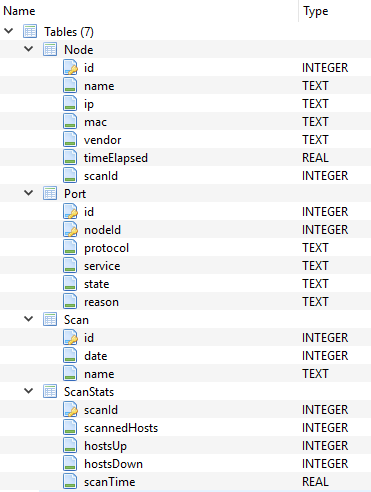
\includegraphics{db-tables}
	\caption{Arquitectura de Room e interrelación entre sus diferentes componentes}
	\label{fig:db-tables}
\end{figure}

Cómo podemos observar solo contamos únicamente con cuatro tablas (se han omitido las tablas generadas automáticamente por Android). Una para cada escaneo, otra para las diferentes estadísticas sobre cada escaneo, otra para que la información de cada nodo y una última para la información de de un puerto de un nodo concreto. Este caso se ha optado por almacenar esta información, pero resultaría fácilmente escalable simplemente añadiendo más campos en nuestra base de datos.

\subsection{Implementación de la base de datos}

Tras tener la base de datos diseñada debemos implementar la nuestra aplicación. Implementar una base de datos en Android se puede hacer de dos maneras.La primera, la manera tradicional, es utilizar la API estándar de Android para interactuar con bases de datos SQLite. Esta manera implica que debemos introducir nuestras sentencias SQL y ejecutarlas nosotros mediante las diferentes funciones y métodos que nos ofrece la API.

Una alternativa a esta API estándar sería el uso de la librería \textit{Room}\footnote{\url{https://developer.android.com/topic/libraries/architecture/room}}. Esta librería es una de las librerías que forman parte de lo que sedenomina Android Architecture Components. los Architecture Components son diferentes librerías pensadas para solucionar problemas que surgen a la hora de desarrollar aplicaciones en Android y simplificar en gran medida el desarrollo de ciertos tipos de funcionalidad.

Room está pensado para abstraernos de toda la lógica de SQL y permitirnos interactuar con la base de datos de una manera más limpia y natural. A abstraer toda esa capa de composición de sentencias SQL para realizar nuestras consultas y modificaciones de la base de datos, el código a mantener resulta muchísimo más sencillo y elegante.

Para lograr esto se basa en una arquitectura compuesta de tres bloques o componentes principales. Dicha arquitectura se puede observar en la FIGURA.

\begin{figure}[H]
	\centering
	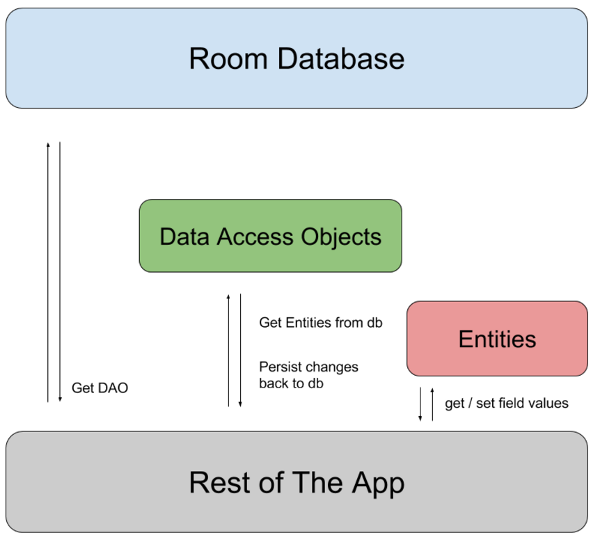
\includegraphics[width=\textwidth]{room-architecture}
	\caption{Arquitectura de Room e interrelación entre sus diferentes componentes}
	\label{fig:room-architecture}
\end{figure}

El primero es el componente \textit{Database}. Este componente es el que nos permite realizar tareas con la base de datos a nivel global. Desde definir las diferentes tablas que pueda haber a obtener la instancia de la base de datos para poder trabajar con ella.

\begin{listing}[H]
	\custominputminted{kotlin}{code/roomDatabase.kt}
	\caption{Implementación de la clase AppDatabase}
	
	\label{code:roomDatabase}
\end{listing}

En el código \ref{code:roomDatabase} se muestra la  implementación de ese componente en nuestra aplicación. Aún no habiendo visto nunca cómo funciona Room se pueden incluir ciertas cosas examinando el código. La primera es que se define mediante anotaciones ciertas clases. Esas clases son las que definen cada una de las tablas que vamos a tener en nuestra base de datos. En Room, las tablas son conocidas como \textit{Entities}, que es otro de los tres componentes de Room. También se puede observar que se añaden una serie de funciones que contienen la nomenclatura \textit{DAO}. Esas funciones son las que nos van a permitir obtener los diferentes DAOs que puedan existir en Room, siendo este tipo de componente el tercero y último.

Como se ha mencionado, las Entities corresponden a cada una de las tablas que existe en la base de datos. Para reflejar esto en una clase de tipo Entity, de la misma manera que se hacía para el componente Database, se utilizan anotaciones.

\begin{listing}[H]
	\custominputminted{kotlin}{code/roomEntities.kt}
	\caption{Implementación de diferentes clases Entity}
	
	\label{code:roomEntities}
\end{listing}

Cómo se puede observar en el ejemplo que se ha puesto en el CÓDIGO, se utilizan anotaciones para definir una entidad o para definir aspectos como la clave primaria de una tabla de la base de datos. Cada uno de los atributos de esa clase equivaldría a un campo de la tabla. Los tipos de datos de la tabla equivalen a los tipos de datos que se han utilizado en los atributos de la clase. Para tipos de atributos complejos Room implementa un componente llamado \textit{Converters} que nos permite implementar funciones que convierten tipos de datos complejos, como imágenes, datos personalizados o clases complejas, en tipos de datos almacenables en una base de datos, de tal manera que se ejecuten automáticamente a la hora de interactuar con la base de datos.

Por último, el tercer componente que se ha mencionado son los \textit{DAO} (Data Access Object). Estos componentes son interfaces que definen una serie de funciones. Esas funciones son la que se utilizarán para hacer consultas o modificaciones en la base de datos. El uso de sentencias SQL como \textit{SELECT}, \textit{INSERT}, \textit{UPDATE} o \textit{DELETE} queda encapsulado mediante el uso de estas funciones, que tanto reciben como devuelven, dependiendo el caso, tipos de datos manipulables a nivel de código. Cada interfaz DAO permite interactuar con una o mas tablas, siendo lo mas recomendable implementar una para cada tabla definida.

\begin{listing}[H]
	\custominputminted{kotlin}{code/roomDao.kt}
	\caption{Ejemplo de una interfaz DAO para interactuar con la base de datos}
	
	\label{code:roomDao}
\end{listing}

Como se puede apreciar en el código \ref{code:roomDao}, mediante anotaciones es donde se especifican las sentencias SQL a las que equivale la ejecución de esas funciones.

Por lo tanto para ejecutar algún tipo de operación en la base datos simplemente hay que combinar estos tres elementos, para disponer de herramientas para definir el modelo de la base de datos e interactuar con la instancia de la base de datos. Por poner unos ejemplos, en los códigos \ref{code:roomSelect} y \ref{code:roomInsert} se muestran partes concretas de la aplicación en las que se realiza una consulta y una inserción en la base de datos, respectivamente.


\begin{listing}[H]
	\custominputminted{kotlin}{code/roomSelect.kt}
	\caption{Ejemplo de obtención de información de la base de datos Room}
	
	\label{code:roomSelect}
\end{listing}

\begin{listing}[H]
	\custominputminted{kotlin}{code/roomInsert.kt}
	\caption{Ejemplo de inserción de información en la base de datos Room}
	
	\label{code:roomInsert}
\end{listing}

Se ha podido ir percibiendo, en ningún momento se ha implementado código que realmente ejecute sentencias SQL. Aquí reside la magia de Room. Room abstrae completamente la programación de ese tipo de código siendo la propia librería quién se encarga de generar ese código a la hora de compilar la aplicación.

Las ventajas de utilizar Room con respecto a la API estándar de SQLite son obvias. Tanto es así que la propia documentación ''recomienda encarecidamente usar Room en vez de SQLite''\cite{room-training}. En primer lugar, abstraemos completamente la generación de código donde concatenamos, generamos y ejecutamos sentencias SQL. Por otra parte, el código que gestiona la base de datos resulta mucho más claro y conciso limitándose a consistir en un par de llamadas a funciones. Por último, la creación de las tablas de la base de datos en sí misma se hace también de manera automática. Incluso tenemos herramientas para poder generar diferentes versiones de la propia base datos a medida que la aplicación vaya escalando, guardándose historiales de versiones de la base de datos para en caso de revertir cambios volver a la estructura de una de las bases de datos anteriores.

\section{Obtención de información de medios externos}

\section{Hilos, Tareas y paralelización}

\section{Interfaz gráfica}



\chapter{Testeo y corrección de errores}

{\color{red} Tras programarlo todo pueden salir fallos, hay que hacer pruebas, e incluso habrá que cambiar cosas o añadir cosas nuevas. Todo eso va explicado aquí. NO CONFUNDIR con añadir nuevos requisitos funcionales o que se haya alargado el tiempo, eso va en la última parte, en la de conclusiones}

\part{Análisis y conclusiones del Trabajo}

\part{Apéndices}


%------------------------------------------------------------------------------

\backmatter

\printbibliography[heading=bibintoc]

%\chapter*{\rlap{GNU Free Documentation License}}
\phantomsection  % so hyperref creates bookmarks
\addcontentsline{toc}{chapter}{GNU Free Documentation License}
%\label{label_fdl}

\begin{center}
	
	Version 1.3, 3 November 2008
	
	
	Copyright \copyright{} 2000, 2001, 2002, 2007, 2008  Free Software Foundation, Inc.
	
	\bigskip
	
	\texttt{<http://fsf.org/>}
	
	\bigskip
	
	Everyone is permitted to copy and distribute verbatim copies
	of this license document, but changing it is not allowed.
\end{center}


\begin{center}
	{\textbf\large Preamble}
\end{center}

The purpose of this License is to make a manual, textbook, or other
functional and useful document ``free'' in the sense of freedom: to
assure everyone the effective freedom to copy and redistribute it,
with or without modifying it, either commercially or noncommercially.
Secondarily, this License preserves for the author and publisher a way
to get credit for their work, while not being considered responsible
for modifications made by others.

This License is a kind of ``copyleft'', which means that derivative
works of the document must themselves be free in the same sense.  It
complements the GNU General Public License, which is a copyleft
license designed for free software.

We have designed this License in order to use it for manuals for free
software, because free software needs free documentation: a free
program should come with manuals providing the same freedoms that the
software does.  But this License is not limited to software manuals;
it can be used for any textual work, regardless of subject matter or
whether it is published as a printed book.  We recommend this License
principally for works whose purpose is instruction or reference.


\begin{center}
	{\Large\textbf 1. APPLICABILITY AND DEFINITIONS\par}
	\phantomsection
	\addcontentsline{toc}{section}{1. APPLICABILITY AND DEFINITIONS}
\end{center}

This License applies to any manual or other work, in any medium, that
contains a notice placed by the copyright holder saying it can be
distributed under the terms of this License.  Such a notice grants a
world-wide, royalty-free license, unlimited in duration, to use that
work under the conditions stated herein.  The ``\textbf{Document}'', below,
refers to any such manual or work.  Any member of the public is a
licensee, and is addressed as ``\textbf{you}''.  You accept the license if you
copy, modify or distribute the work in a way requiring permission
under copyright law.

A ``\textbf{Modified Version}'' of the Document means any work containing the
Document or a portion of it, either copied verbatim, or with
modifications and/or translated into another language.

A ``\textbf{Secondary Section}'' is a named appendix or a front-matter section of
the Document that deals exclusively with the relationship of the
publishers or authors of the Document to the Document's overall subject
(or to related matters) and contains nothing that could fall directly
within that overall subject.  (Thus, if the Document is in part a
textbook of mathematics, a Secondary Section may not explain any
mathematics.)  The relationship could be a matter of historical
connection with the subject or with related matters, or of legal,
commercial, philosophical, ethical or political position regarding
them.

The ``\textbf{Invariant Sections}'' are certain Secondary Sections whose titles
are designated, as being those of Invariant Sections, in the notice
that says that the Document is released under this License.  If a
section does not fit the above definition of Secondary then it is not
allowed to be designated as Invariant.  The Document may contain zero
Invariant Sections.  If the Document does not identify any Invariant
Sections then there are none.

The ``\textbf{Cover Texts}'' are certain short passages of text that are listed,
as Front-Cover Texts or Back-Cover Texts, in the notice that says that
the Document is released under this License.  A Front-Cover Text may
be at most 5 words, and a Back-Cover Text may be at most 25 words.

A ``\textbf{Transparent}'' copy of the Document means a machine-readable copy,
represented in a format whose specification is available to the
general public, that is suitable for revising the document
straightforwardly with generic text editors or (for images composed of
pixels) generic paint programs or (for drawings) some widely available
drawing editor, and that is suitable for input to text formatters or
for automatic translation to a variety of formats suitable for input
to text formatters.  A copy made in an otherwise Transparent file
format whose markup, or absence of markup, has been arranged to thwart
or discourage subsequent modification by readers is not Transparent.
An image format is not Transparent if used for any substantial amount
of text.  A copy that is not ``Transparent'' is called ``\textbf{Opaque}''.

Examples of suitable formats for Transparent copies include plain
ASCII without markup, Texinfo input format, LaTeX input format, SGML
or XML using a publicly available DTD, and standard-conforming simple
HTML, PostScript or PDF designed for human modification.  Examples of
transparent image formats include PNG, XCF and JPG.  Opaque formats
include proprietary formats that can be read and edited only by
proprietary word processors, SGML or XML for which the DTD and/or
processing tools are not generally available, and the
machine-generated HTML, PostScript or PDF produced by some word
processors for output purposes only.

The ``\textbf{Title Page}'' means, for a printed book, the title page itself,
plus such following pages as are needed to hold, legibly, the material
this License requires to appear in the title page.  For works in
formats which do not have any title page as such, ``Title Page'' means
the text near the most prominent appearance of the work's title,
preceding the beginning of the body of the text.

The ``\textbf{publisher}'' means any person or entity that distributes
copies of the Document to the public.

A section ``\textbf{Entitled XYZ}'' means a named subunit of the Document whose
title either is precisely XYZ or contains XYZ in parentheses following
text that translates XYZ in another language.  (Here XYZ stands for a
specific section name mentioned below, such as ``\textbf{Acknowledgements}'',
``\textbf{Dedications}'', ``\textbf{Endorsements}'', or ``\textbf{History}''.)  
To ``\textbf{Preserve the Title}''
of such a section when you modify the Document means that it remains a
section ``Entitled XYZ'' according to this definition.

The Document may include Warranty Disclaimers next to the notice which
states that this License applies to the Document.  These Warranty
Disclaimers are considered to be included by reference in this
License, but only as regards disclaiming warranties: any other
implication that these Warranty Disclaimers may have is void and has
no effect on the meaning of this License.


\begin{center}
	{\Large\textbf 2. VERBATIM COPYING\par}
	\phantomsection
	\addcontentsline{toc}{section}{2. VERBATIM COPYING}
\end{center}

You may copy and distribute the Document in any medium, either
commercially or noncommercially, provided that this License, the
copyright notices, and the license notice saying this License applies
to the Document are reproduced in all copies, and that you add no other
conditions whatsoever to those of this License.  You may not use
technical measures to obstruct or control the reading or further
copying of the copies you make or distribute.  However, you may accept
compensation in exchange for copies.  If you distribute a large enough
number of copies you must also follow the conditions in section~3.

You may also lend copies, under the same conditions stated above, and
you may publicly display copies.


\begin{center}
	{\Large\textbf 3. COPYING IN QUANTITY\par}
	\phantomsection
	\addcontentsline{toc}{section}{3. COPYING IN QUANTITY}
\end{center}


If you publish printed copies (or copies in media that commonly have
printed covers) of the Document, numbering more than 100, and the
Document's license notice requires Cover Texts, you must enclose the
copies in covers that carry, clearly and legibly, all these Cover
Texts: Front-Cover Texts on the front cover, and Back-Cover Texts on
the back cover.  Both covers must also clearly and legibly identify
you as the publisher of these copies.  The front cover must present
the full title with all words of the title equally prominent and
visible.  You may add other material on the covers in addition.
Copying with changes limited to the covers, as long as they preserve
the title of the Document and satisfy these conditions, can be treated
as verbatim copying in other respects.

If the required texts for either cover are too voluminous to fit
legibly, you should put the first ones listed (as many as fit
reasonably) on the actual cover, and continue the rest onto adjacent
pages.

If you publish or distribute Opaque copies of the Document numbering
more than 100, you must either include a machine-readable Transparent
copy along with each Opaque copy, or state in or with each Opaque copy
a computer-network location from which the general network-using
public has access to download using public-standard network protocols
a complete Transparent copy of the Document, free of added material.
If you use the latter option, you must take reasonably prudent steps,
when you begin distribution of Opaque copies in quantity, to ensure
that this Transparent copy will remain thus accessible at the stated
location until at least one year after the last time you distribute an
Opaque copy (directly or through your agents or retailers) of that
edition to the public.

It is requested, but not required, that you contact the authors of the
Document well before redistributing any large number of copies, to give
them a chance to provide you with an updated version of the Document.


\begin{center}
	{\Large\textbf 4. MODIFICATIONS\par}
	\phantomsection
	\addcontentsline{toc}{section}{4. MODIFICATIONS}
\end{center}

You may copy and distribute a Modified Version of the Document under
the conditions of sections 2 and 3 above, provided that you release
the Modified Version under precisely this License, with the Modified
Version filling the role of the Document, thus licensing distribution
and modification of the Modified Version to whoever possesses a copy
of it.  In addition, you must do these things in the Modified Version:

\begin{itemize}
	\item[A.] 
	Use in the Title Page (and on the covers, if any) a title distinct
	from that of the Document, and from those of previous versions
	(which should, if there were any, be listed in the History section
	of the Document).  You may use the same title as a previous version
	if the original publisher of that version gives permission.
	
	\item[B.]
	List on the Title Page, as authors, one or more persons or entities
	responsible for authorship of the modifications in the Modified
	Version, together with at least five of the principal authors of the
	Document (all of its principal authors, if it has fewer than five),
	unless they release you from this requirement.
	
	\item[C.]
	State on the Title page the name of the publisher of the
	Modified Version, as the publisher.
	
	\item[D.]
	Preserve all the copyright notices of the Document.
	
	\item[E.]
	Add an appropriate copyright notice for your modifications
	adjacent to the other copyright notices.
	
	\item[F.]
	Include, immediately after the copyright notices, a license notice
	giving the public permission to use the Modified Version under the
	terms of this License, in the form shown in the Addendum below.
	
	\item[G.]
	Preserve in that license notice the full lists of Invariant Sections
	and required Cover Texts given in the Document's license notice.
	
	\item[H.]
	Include an unaltered copy of this License.
	
	\item[I.]
	Preserve the section Entitled ``History'', Preserve its Title, and add
	to it an item stating at least the title, year, new authors, and
	publisher of the Modified Version as given on the Title Page.  If
	there is no section Entitled ``History'' in the Document, create one
	stating the title, year, authors, and publisher of the Document as
	given on its Title Page, then add an item describing the Modified
	Version as stated in the previous sentence.
	
	\item[J.]
	Preserve the network location, if any, given in the Document for
	public access to a Transparent copy of the Document, and likewise
	the network locations given in the Document for previous versions
	it was based on.  These may be placed in the ``History'' section.
	You may omit a network location for a work that was published at
	least four years before the Document itself, or if the original
	publisher of the version it refers to gives permission.
	
	\item[K.]
	For any section Entitled ``Acknowledgements'' or ``Dedications'',
	Preserve the Title of the section, and preserve in the section all
	the substance and tone of each of the contributor acknowledgements
	and/or dedications given therein.
	
	\item[L.]
	Preserve all the Invariant Sections of the Document,
	unaltered in their text and in their titles.  Section numbers
	or the equivalent are not considered part of the section titles.
	
	\item[M.]
	Delete any section Entitled ``Endorsements''.  Such a section
	may not be included in the Modified Version.
	
	\item[N.]
	Do not retitle any existing section to be Entitled ``Endorsements''
	or to conflict in title with any Invariant Section.
	
	\item[O.]
	Preserve any Warranty Disclaimers.
\end{itemize}

If the Modified Version includes new front-matter sections or
appendices that qualify as Secondary Sections and contain no material
copied from the Document, you may at your option designate some or all
of these sections as invariant.  To do this, add their titles to the
list of Invariant Sections in the Modified Version's license notice.
These titles must be distinct from any other section titles.

You may add a section Entitled ``Endorsements'', provided it contains
nothing but endorsements of your Modified Version by various
parties---for example, statements of peer review or that the text has
been approved by an organization as the authoritative definition of a
standard.

You may add a passage of up to five words as a Front-Cover Text, and a
passage of up to 25 words as a Back-Cover Text, to the end of the list
of Cover Texts in the Modified Version.  Only one passage of
Front-Cover Text and one of Back-Cover Text may be added by (or
through arrangements made by) any one entity.  If the Document already
includes a cover text for the same cover, previously added by you or
by arrangement made by the same entity you are acting on behalf of,
you may not add another; but you may replace the old one, on explicit
permission from the previous publisher that added the old one.

The author(s) and publisher(s) of the Document do not by this License
give permission to use their names for publicity for or to assert or
imply endorsement of any Modified Version.


\begin{center}
	{\Large\textbf 5. COMBINING DOCUMENTS\par}
	\phantomsection
	\addcontentsline{toc}{section}{5. COMBINING DOCUMENTS}
\end{center}


You may combine the Document with other documents released under this
License, under the terms defined in section~4 above for modified
versions, provided that you include in the combination all of the
Invariant Sections of all of the original documents, unmodified, and
list them all as Invariant Sections of your combined work in its
license notice, and that you preserve all their Warranty Disclaimers.

The combined work need only contain one copy of this License, and
multiple identical Invariant Sections may be replaced with a single
copy.  If there are multiple Invariant Sections with the same name but
different contents, make the title of each such section unique by
adding at the end of it, in parentheses, the name of the original
author or publisher of that section if known, or else a unique number.
Make the same adjustment to the section titles in the list of
Invariant Sections in the license notice of the combined work.

In the combination, you must combine any sections Entitled ``History''
in the various original documents, forming one section Entitled
``History''; likewise combine any sections Entitled ``Acknowledgements'',
and any sections Entitled ``Dedications''.  You must delete all sections
Entitled ``Endorsements''.

\begin{center}
	{\Large\textbf 6. COLLECTIONS OF DOCUMENTS\par}
	\phantomsection
	\addcontentsline{toc}{section}{6. COLLECTIONS OF DOCUMENTS}
\end{center}

You may make a collection consisting of the Document and other documents
released under this License, and replace the individual copies of this
License in the various documents with a single copy that is included in
the collection, provided that you follow the rules of this License for
verbatim copying of each of the documents in all other respects.

You may extract a single document from such a collection, and distribute
it individually under this License, provided you insert a copy of this
License into the extracted document, and follow this License in all
other respects regarding verbatim copying of that document.


\begin{center}
	{\Large\textbf 7. AGGREGATION WITH INDEPENDENT WORKS\par}
	\phantomsection
	\addcontentsline{toc}{section}{7. AGGREGATION WITH INDEPENDENT WORKS}
\end{center}


A compilation of the Document or its derivatives with other separate
and independent documents or works, in or on a volume of a storage or
distribution medium, is called an ``aggregate'' if the copyright
resulting from the compilation is not used to limit the legal rights
of the compilation's users beyond what the individual works permit.
When the Document is included in an aggregate, this License does not
apply to the other works in the aggregate which are not themselves
derivative works of the Document.

If the Cover Text requirement of section~3 is applicable to these
copies of the Document, then if the Document is less than one half of
the entire aggregate, the Document's Cover Texts may be placed on
covers that bracket the Document within the aggregate, or the
electronic equivalent of covers if the Document is in electronic form.
Otherwise they must appear on printed covers that bracket the whole
aggregate.


\begin{center}
	{\Large\textbf 8. TRANSLATION\par}
	\phantomsection
	\addcontentsline{toc}{section}{8. TRANSLATION}
\end{center}


Translation is considered a kind of modification, so you may
distribute translations of the Document under the terms of section~4.
Replacing Invariant Sections with translations requires special
permission from their copyright holders, but you may include
translations of some or all Invariant Sections in addition to the
original versions of these Invariant Sections.  You may include a
translation of this License, and all the license notices in the
Document, and any Warranty Disclaimers, provided that you also include
the original English version of this License and the original versions
of those notices and disclaimers.  In case of a disagreement between
the translation and the original version of this License or a notice
or disclaimer, the original version will prevail.

If a section in the Document is Entitled ``Acknowledgements'',
``Dedications'', or ``History'', the requirement (section~4) to Preserve
its Title (section~1) will typically require changing the actual
title.


\begin{center}
	{\Large\textbf 9. TERMINATION\par}
	\phantomsection
	\addcontentsline{toc}{section}{9. TERMINATION}
\end{center}


You may not copy, modify, sublicense, or distribute the Document
except as expressly provided under this License.  Any attempt
otherwise to copy, modify, sublicense, or distribute it is void, and
will automatically terminate your rights under this License.

However, if you cease all violation of this License, then your license
from a particular copyright holder is reinstated (a) provisionally,
unless and until the copyright holder explicitly and finally
terminates your license, and (b) permanently, if the copyright holder
fails to notify you of the violation by some reasonable means prior to
60 days after the cessation.

Moreover, your license from a particular copyright holder is
reinstated permanently if the copyright holder notifies you of the
violation by some reasonable means, this is the first time you have
received notice of violation of this License (for any work) from that
copyright holder, and you cure the violation prior to 30 days after
your receipt of the notice.

Termination of your rights under this section does not terminate the
licenses of parties who have received copies or rights from you under
this License.  If your rights have been terminated and not permanently
reinstated, receipt of a copy of some or all of the same material does
not give you any rights to use it.


\begin{center}
	{\Large\textbf 10. FUTURE REVISIONS OF THIS LICENSE\par}
	\phantomsection
	\addcontentsline{toc}{section}{10. FUTURE REVISIONS OF THIS LICENSE}
\end{center}


The Free Software Foundation may publish new, revised versions
of the GNU Free Documentation License from time to time.  Such new
versions will be similar in spirit to the present version, but may
differ in detail to address new problems or concerns.  See
\texttt{http://www.gnu.org/copyleft/}.

Each version of the License is given a distinguishing version number.
If the Document specifies that a particular numbered version of this
License ``or any later version'' applies to it, you have the option of
following the terms and conditions either of that specified version or
of any later version that has been published (not as a draft) by the
Free Software Foundation.  If the Document does not specify a version
number of this License, you may choose any version ever published (not
as a draft) by the Free Software Foundation.  If the Document
specifies that a proxy can decide which future versions of this
License can be used, that proxy's public statement of acceptance of a
version permanently authorizes you to choose that version for the
Document.


\begin{center}
	{\Large\textbf 11. RELICENSING\par}
	\phantomsection
	\addcontentsline{toc}{section}{11. RELICENSING}
\end{center}


``Massive Multiauthor Collaboration Site'' (or ``MMC Site'') means any
World Wide Web server that publishes copyrightable works and also
provides prominent facilities for anybody to edit those works.  A
public wiki that anybody can edit is an example of such a server.  A
``Massive Multiauthor Collaboration'' (or ``MMC'') contained in the
site means any set of copyrightable works thus published on the MMC
site.

``CC-BY-SA'' means the Creative Commons Attribution-Share Alike 3.0
license published by Creative Commons Corporation, a not-for-profit
corporation with a principal place of business in San Francisco,
California, as well as future copyleft versions of that license
published by that same organization.

``Incorporate'' means to publish or republish a Document, in whole or
in part, as part of another Document.

An MMC is ``eligible for relicensing'' if it is licensed under this
License, and if all works that were first published under this License
somewhere other than this MMC, and subsequently incorporated in whole
or in part into the MMC, (1) had no cover texts or invariant sections,
and (2) were thus incorporated prior to November 1, 2008.

The operator of an MMC Site may republish an MMC contained in the site
under CC-BY-SA on the same site at any time before August 1, 2009,
provided the MMC is eligible for relicensing.


\begin{center}
	{\Large\textbf ADDENDUM: How to use this License for your documents\par}
	\phantomsection
	\addcontentsline{toc}{section}{ADDENDUM: How to use this License for your documents}
\end{center}

To use this License in a document you have written, include a copy of
the License in the document and put the following copyright and
license notices just after the title page:

\bigskip
\begin{quote}
	Copyright \copyright{}  YEAR  YOUR NAME.
	Permission is granted to copy, distribute and/or modify this document
	under the terms of the GNU Free Documentation License, Version 1.3
	or any later version published by the Free Software Foundation;
	with no Invariant Sections, no Front-Cover Texts, and no Back-Cover Texts.
	A copy of the license is included in the section entitled ``GNU
	Free Documentation License''.
\end{quote}
\bigskip

If you have Invariant Sections, Front-Cover Texts and Back-Cover Texts,
replace the ``with \dots\ Texts.''\ line with this:

\bigskip
\begin{quote}
	with the Invariant Sections being LIST THEIR TITLES, with the
	Front-Cover Texts being LIST, and with the Back-Cover Texts being LIST.
\end{quote}
\bigskip

If you have Invariant Sections without Cover Texts, or some other
combination of the three, merge those two alternatives to suit the
situation.

If your document contains nontrivial examples of program code, we
recommend releasing these examples in parallel under your choice of
free software license, such as the GNU General Public License,
to permit their use in free software.

\end{document}
%==============================================================================